\chapter{Optimization Results}
\section{NASA CRM Optimization}
\subsection{NASA CRM Optimization with Wing Twist}
\label{ssec:crm-opt-twist}
The initial optimization of the CRM geometry was carried out using the procedure outlined in section~\ref{ssec-prob-formulate}. Observation of the design variable history during optimization iterations illustrated that the wing sweep rose to its upper limit of 45.9\degree\ within 50 iterations and remained there. The optimization was manually stopped after 78 design iterations. Analysis of the merit function, optimality, and feasibility of this study illustrated that this case was not converged, as seen in Figure~\ref{fig:crm_converge_45.9_Deg}.
\begin{figure}[ht!]
\centering
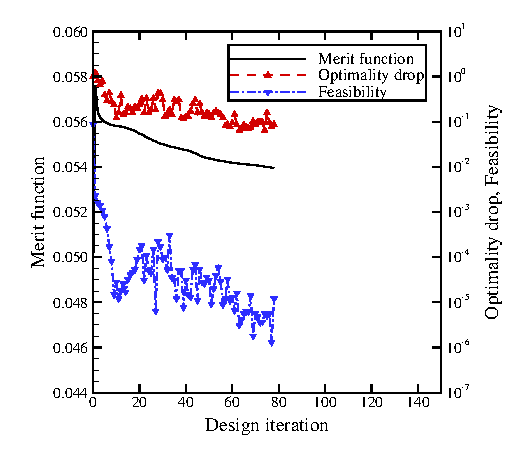
\includegraphics[width=4.5in]{Figures/With_Twist/CRM/optimize_CRM.eps}
\caption{Convergence history for NASA-CRM optimization with an upper sweep angle limit of 45.9\degree.}
\label{fig:crm_converge_45.9_Deg}
\end{figure}
Despite insufficient convergence, it was clear that this geometry had a very strong tendency to increase the wing sweep even further, as evidenced by the active wing sweep constraint very early on in the optimization. Performance had also greatly increased when compared to a baseline flow solution for the same geometry, which was trimmed to an angle of attack that would satisfy the lift constraint of $C_L S=1.6972$, as seen in Table~\ref{tab:crm_results}. The drag coefficient $C_D S$ had decreased by 50.5 drag counts with a small decrease in angle of attack. The $L/D$ had also increased by over 2.5 from 28.78 to 31.48. This substantial improvement in efficiency motivated the decision to halt the optimization and completely restart it with an increased sweep angle limit, as better performing optima may be located at higher sweep angles.


\begin{table}[!tp]
\centering
\caption{Results summary for the optimization of the NASA CRM}
\label{tab:crm_results}
\begin{adjustbox}{center}
\begin{tabular}{lcccc}
\hline\hline
Design Variable & Trimmed Baseline & 45.9\degree\ Sweep Limit & 50.0\degree\ Sweep Limit & 60.0\degree\ Sweep Limit\\
\hline
$S$ (ref. units\textsuperscript{2}) & 3.395 & 3.388 & 3.385 & 3.384 \\
$C_L S$ & 1.6972 & 1.6972 & 1.6972 & 1.6972 \\
$C_M S$ & -2.704 & -3.439 & -3.837 & -3.842 \\
$C_D S$ (counts) & 589.7 & 539.2 & 529.4 & 528.8 \\
$L/D$ & 28.78 & 31.48 & 32.06 & 32.08 \\
Angle of Attack & 1.982\degree\ & 1.436\degree\ & 0.909\degree\ & 0.848\degree\ \\
\makecell[l]{Post-Optimization\\Leading Edge Sweep Angle} & 37.50\degree\ & 45.77\degree\ & 49.16\degree\ & 49.05\degree\ \\
\hline\hline
\end{tabular}
\end{adjustbox}
\end{table}

The second case was run with a sweep angle limit expanded to 50\degree, which after converting to units of MAC and truncating, resulted in an increased upper sweep angle limit of 50.0\degree.
This case was run for over 200 iterations, with continual decreases in the merit function and feasibility observed, as seen in Figure~\ref{fig:crm_converge_50.0_Deg}. However, the optimality struggled to drop further than $10^{-1}$ below its original value.

Analysis of the optimization iteration history illustrated that the optimized geometry possesses a sweep angle very close to the sweep angle limit of 50.0\degree. The sweep angle had increased to 49.16\degree, with further improvements in $C_D S$ by 9.8 drag counts over the 45.9\degree\ sweep limit case. Meanwhile, the angle of attack decreased by over 0.5\degree, dropping from 1.436\degree\ to 0.909\degree. When converted to units of MAC, the margin between the optimized sweep angle and the upper sweep angle limit was just 0.131 reference units. This value is only 8\% of the 50.0\degree\ sweep angle limit of 1.600 reference units. Given this small margin, the continued performance improvements at higher sweep angles, and the strong decrease observed in the feasibility past 200 design iterations in Figure~\ref{fig:crm_converge_50.0_Deg}, it was decided that the sweep angle should be increased further as there may yet be better performance to be obtained.

\begin{figure}[!tp]
\centering
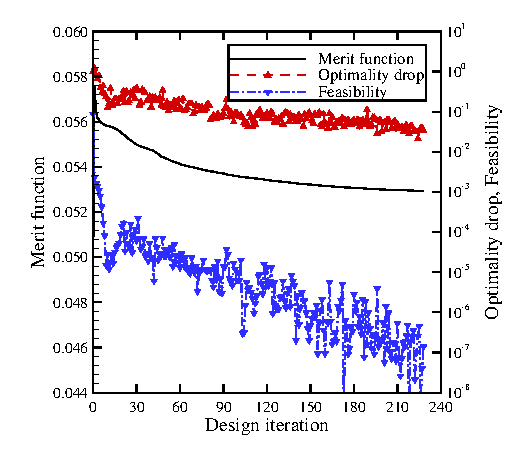
\includegraphics[width=4.5in]{Figures/With_Twist/CRM/Optimize_CRM_50deg.eps}
\caption{Convergence history for NASA-CRM optimization with an upper sweep angle limit of 50.0\degree.}
\label{fig:crm_converge_50.0_Deg}
\end{figure}

The last CRM case to be run made use of the last optimized geometry from the 50.0\degree\ sweep angle limit case as its initial geometry. The upper sweep angle limit was expanded further to 60.0\degree. This case was run for 60 iterations and observed no substantial changes to the merit function and optimality, whereas the feasibility decreased by one order of magnitude to approximately $10^{-8}$, as seen in Figure~\ref{fig:crm_converge_60.0_Deg}.

\begin{figure}[!tp]
\centering
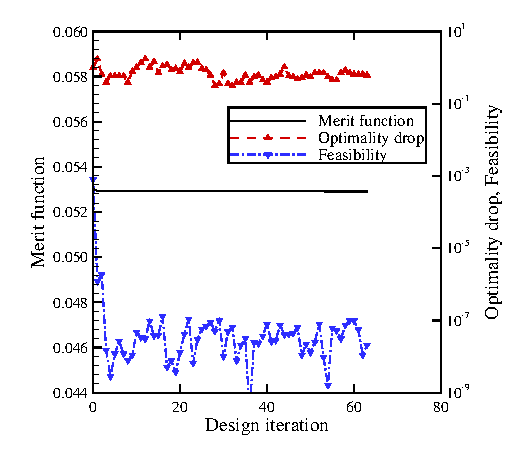
\includegraphics[width=4.5in]{Figures/With_Twist/CRM/Optimize_CRM_60deg.eps}
\caption{Convergence history for NASA-CRM optimization with an upper sweep angle limit of 60.0\degree.}
\label{fig:crm_converge_60.0_Deg}
\end{figure}
Performance for this geometry did not change significantly compared to the 50.0\degree\ sweep angle limit case. The $C_D S$ decreased by 0.6 drag counts to 528.8, the $L/D$ increased by 0.02 to 32.08, and the angle of attack decreased by 0.061\degree\ to 0.848\degree, as seen in Table~\ref{tab:crm_results}. Notably, the sweep angle decreased from the 50.0\degree\ case's most optimal point, dropping 0.1\degree\ from 49.16\degree\ to 49.05\degree, indicating further convergence towards the optimum obtained in the 50.0\degree sweep limit case.

Plots of the upper surface pressure contours for the 60.0\degree\ sweep angle limit optimized planform and the baseline flow solution—trimmed to an angle of attack that satisfies the lift constraint (trimmed angle of attack baseline)—are shown in Figure~\ref{fig:crm_planform_plots}. Plots of the section geometry and pressure distribution at various spanwise sections for the 60.0\degree\ sweep angle limit optimized planform and the trimmed angle of attack baseline are shown in Figure~\ref{fig:crm_section_plots}.

\begin{figure}[!tp]
    \centering
    \subfloat[\label{fig:crm_baseline_planform}]{\includegraphics[trim={0.25cm 0.25cm 0.25cm 0.25cm},clip,width=3.175in]{Figures/With_Twist/CRM/NASA_CRM_Baseline_Trimmed-Contour-Upper.eps}}
    \hspace{0.25cm}
    \subfloat[\label{fig:crm_60_deg_planform}]{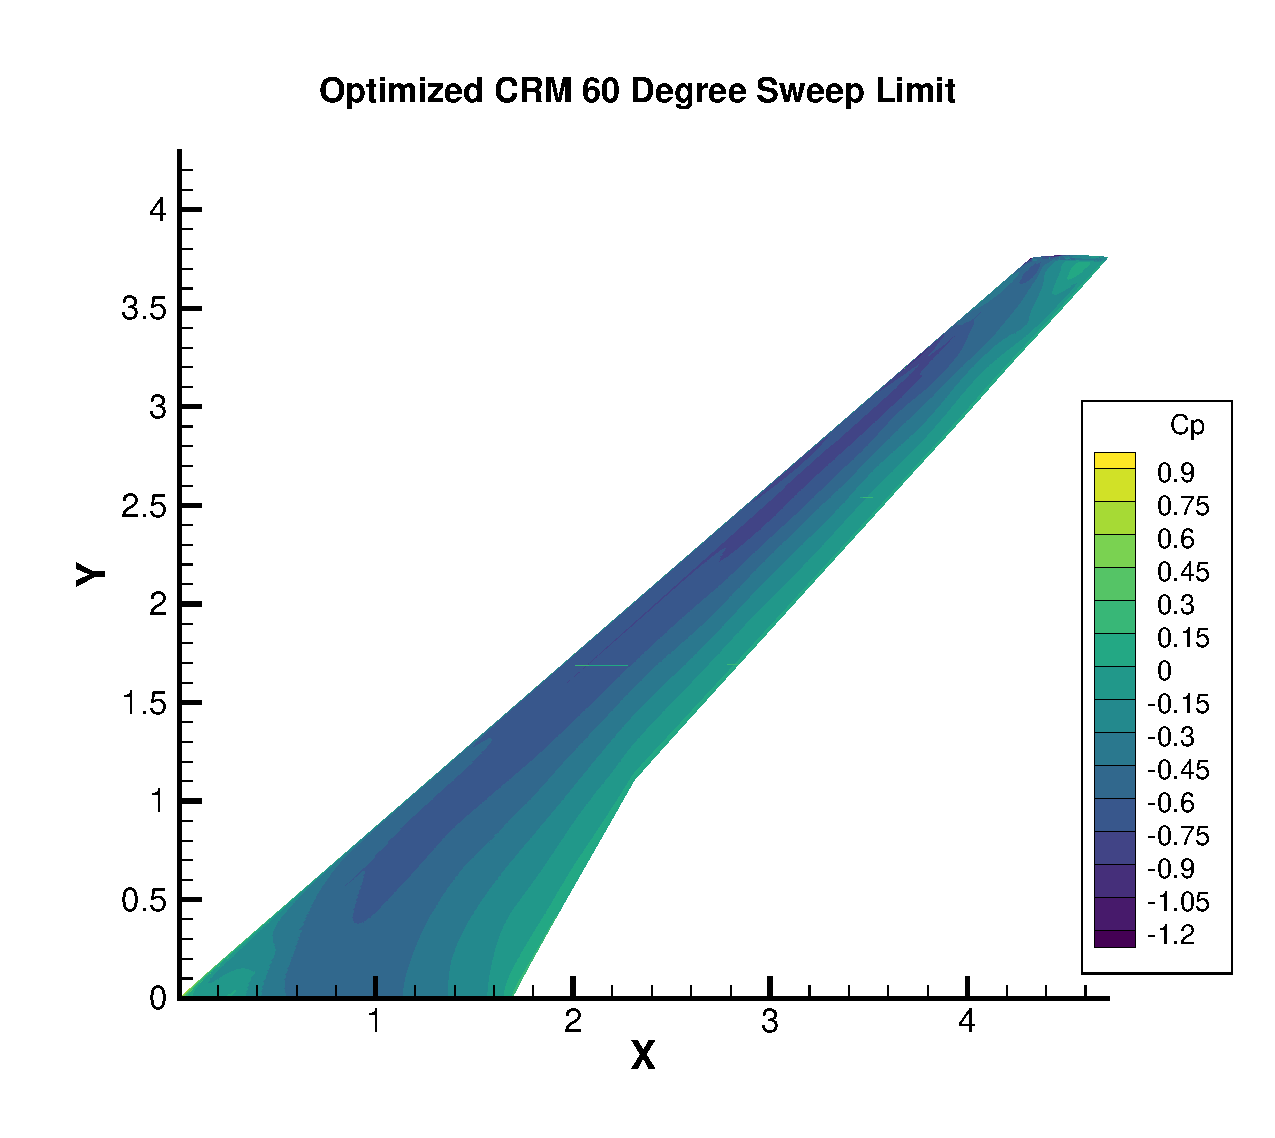
\includegraphics[trim={0.25cm 0.25cm 0.25cm 0.25cm},clip,width=3.175in]{Figures/With_Twist/CRM/NASA_CRM_varsweep_60deg-Contour-Upper.eps}}
    \caption{Upper surface pressure contours for the trimmed angle of attack baseline planform (\ref{fig:crm_baseline_planform}) and the 60.0\degree\ sweep angle limit optimized planform (\ref{fig:crm_60_deg_planform}).}
\label{fig:crm_planform_plots}
\end{figure}

\begin{figure}[!tp]
    \centering
    \subfloat[\label{fig:crm_section_1_perc}]{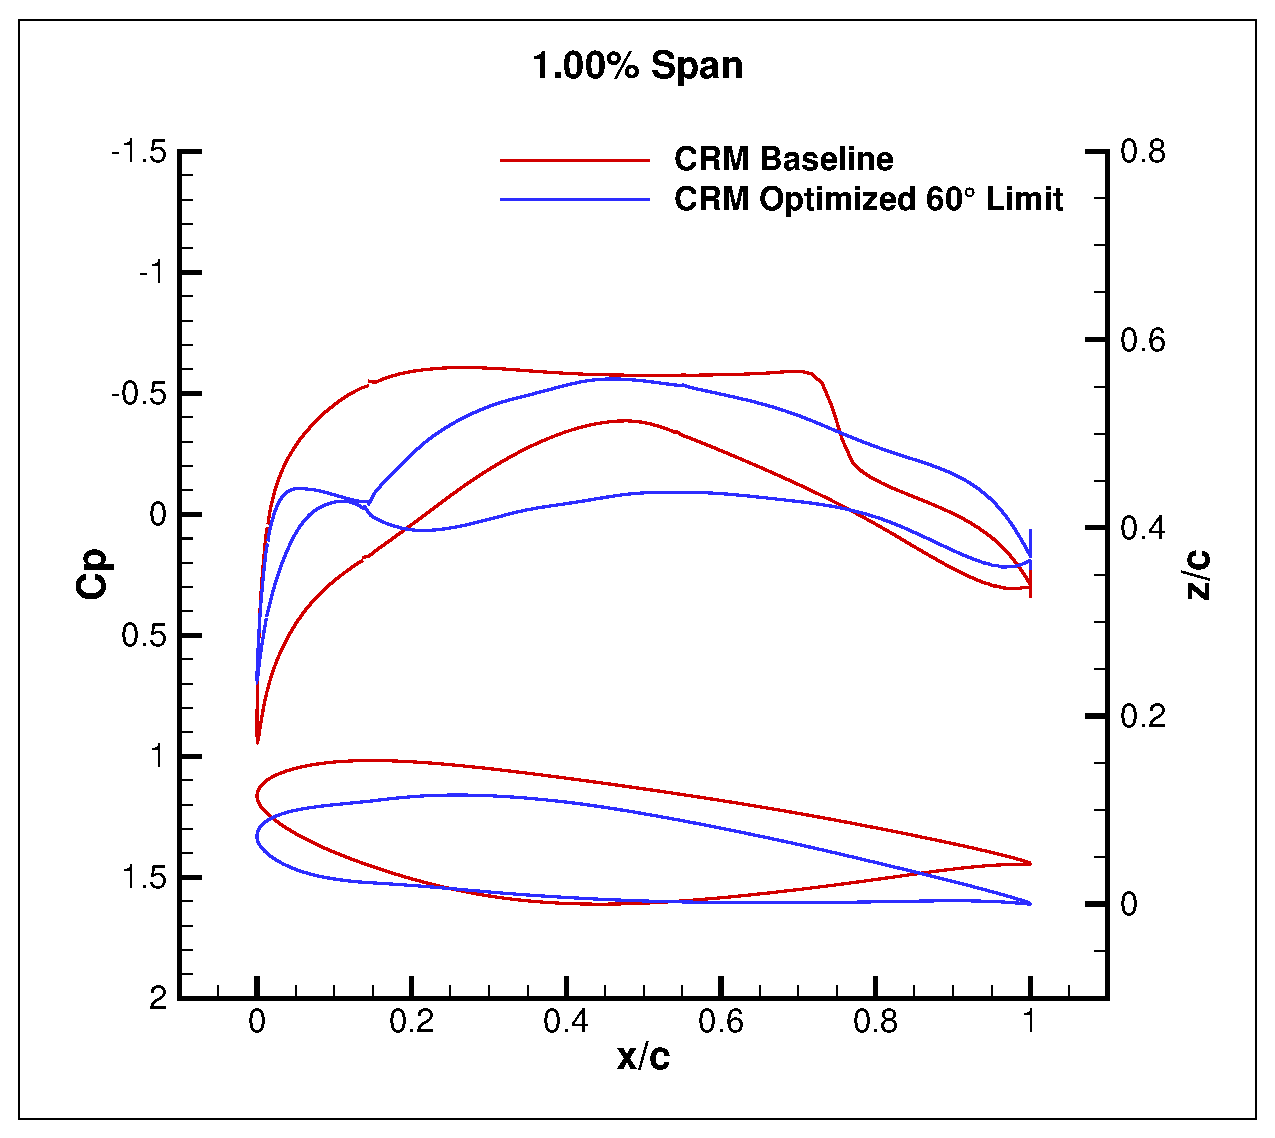
\includegraphics[trim={0.25cm 0.25cm 0.25cm 0.25cm},clip,width=3in]{Figures/With_Twist/CRM/NASA_CRM_Optimize_60deg-1percent_Span.eps}}
    \hspace{0.25cm}
    \subfloat[\label{fig:crm_section_20.6_perc}]{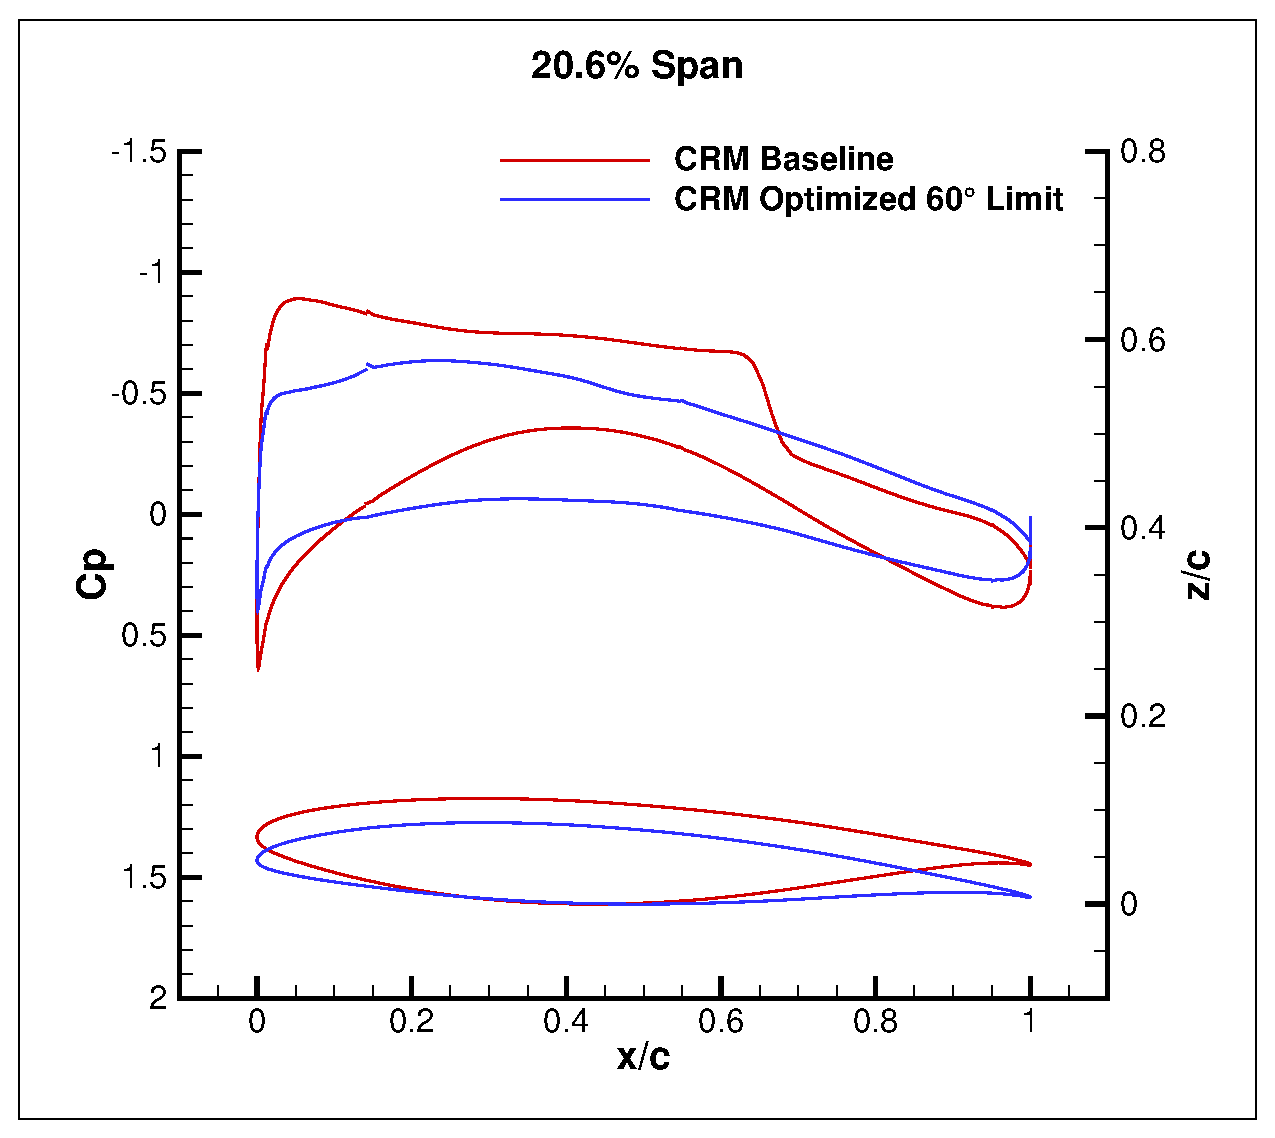
\includegraphics[trim={0.25cm 0.25cm 0.25cm 0.25cm},clip,width=3in]{Figures/With_Twist/CRM/NASA_CRM_Optimize_60deg-20.6percent_Span.eps}}\\
    \subfloat[\label{fig:crm_section_40.2_perc}]{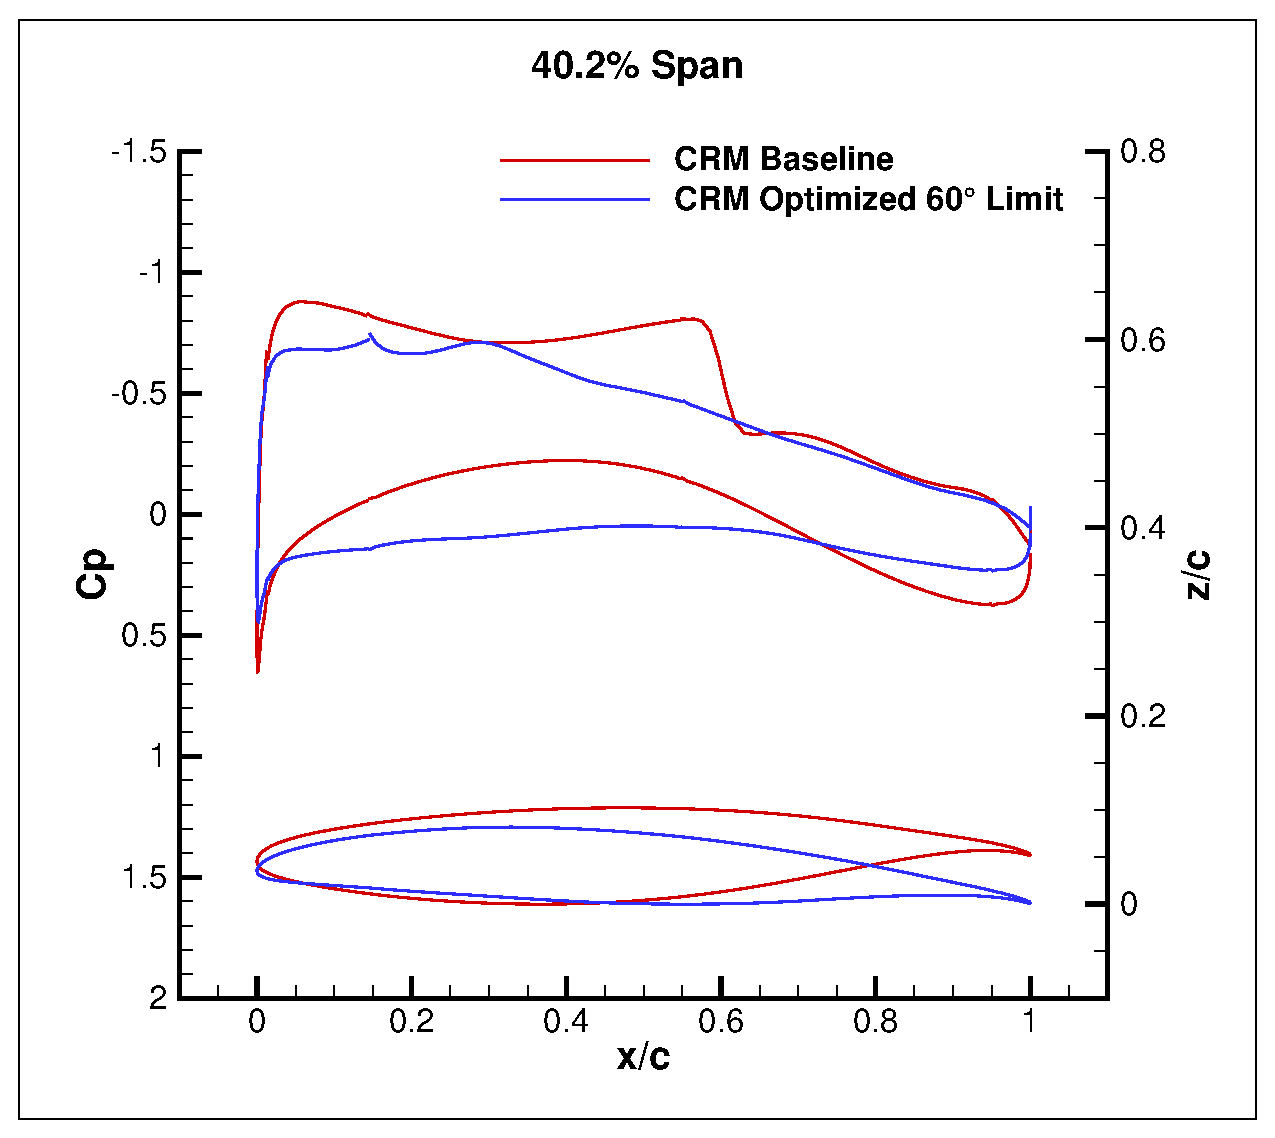
\includegraphics[trim={0.25cm 0.25cm 0.25cm 0.25cm},clip,width=3in]{Figures/With_Twist/CRM/NASA_CRM_Optimize_60deg-40.2percent_Span.eps}}
    \hspace{0.25cm}
    \subfloat[\label{fig:crm_section_59.8_perc}]{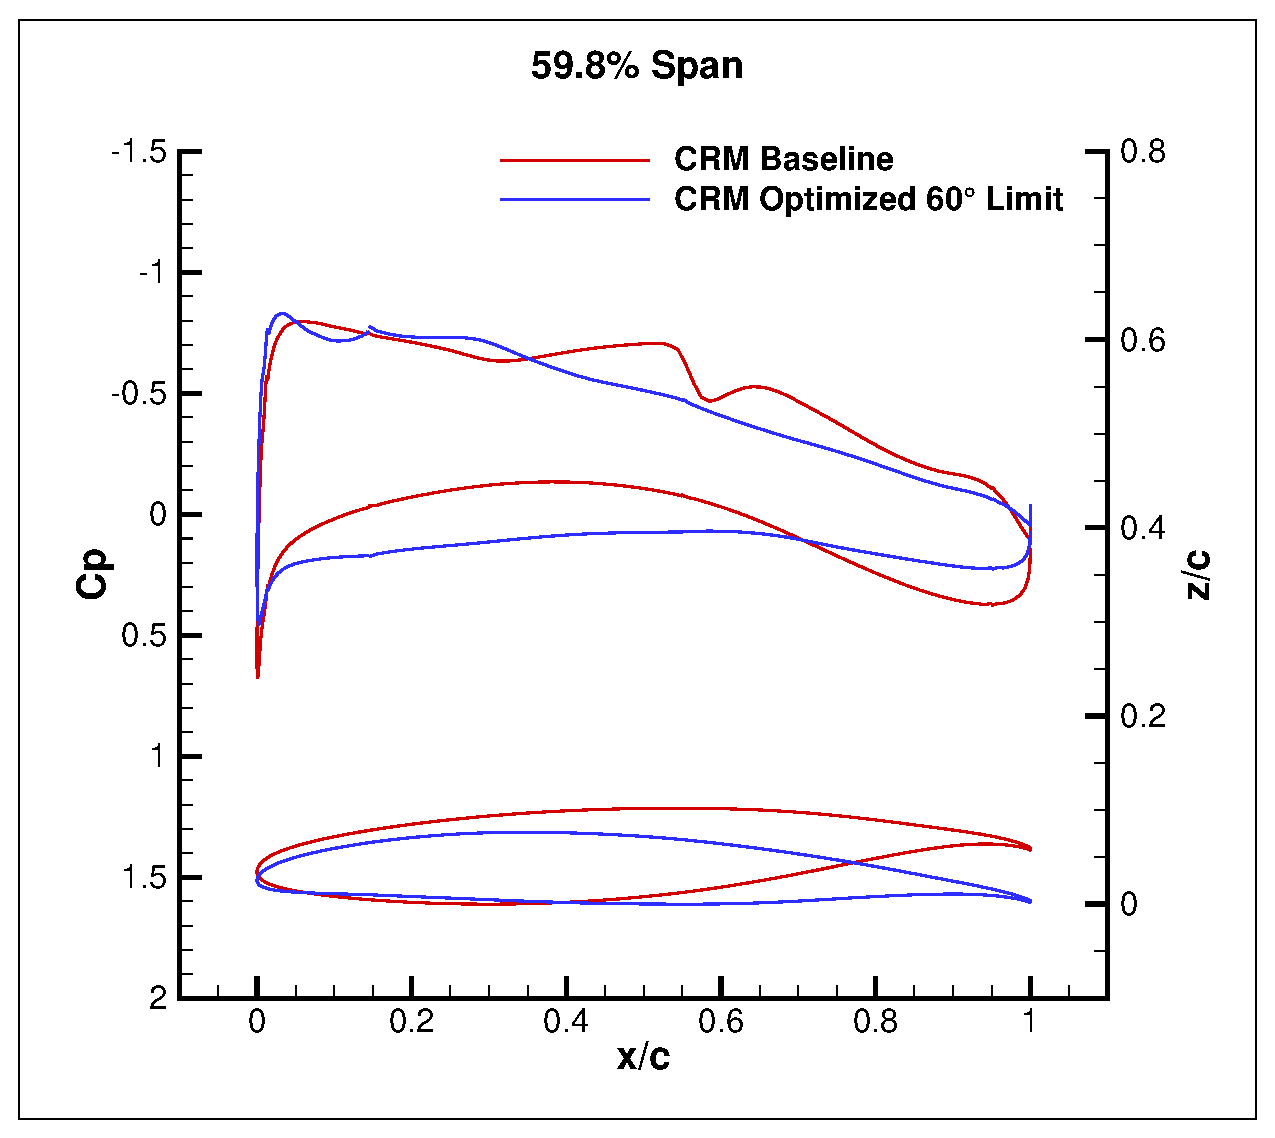
\includegraphics[trim={0.25cm 0.25cm 0.25cm 0.25cm},clip,width=3in]{Figures/With_Twist/CRM/NASA_CRM_Optimize_60deg-59.8percent_Span.eps}}\\
    \subfloat[\label{fig:crm_section_79.4_perc}]{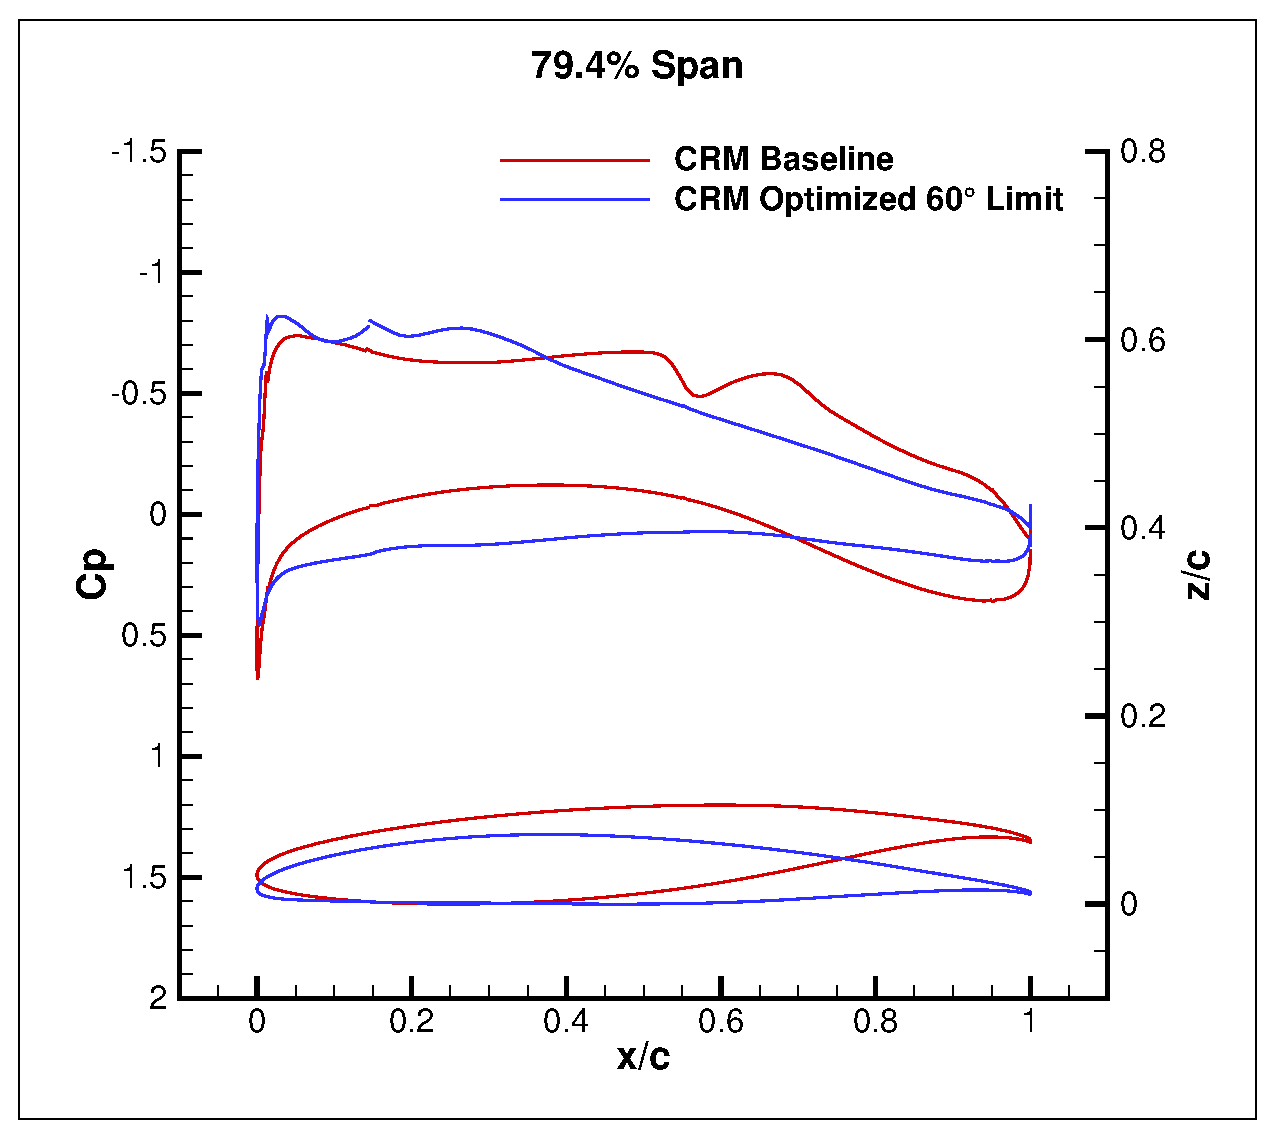
\includegraphics[trim={0.25cm 0.25cm 0.25cm 0.25cm},clip,width=3in]{Figures/With_Twist/CRM/NASA_CRM_Optimize_60deg-79.4percent_Span.eps}}
    \hspace{0.25cm}
    \subfloat[\label{fig:crm_section_99.0_perc}]{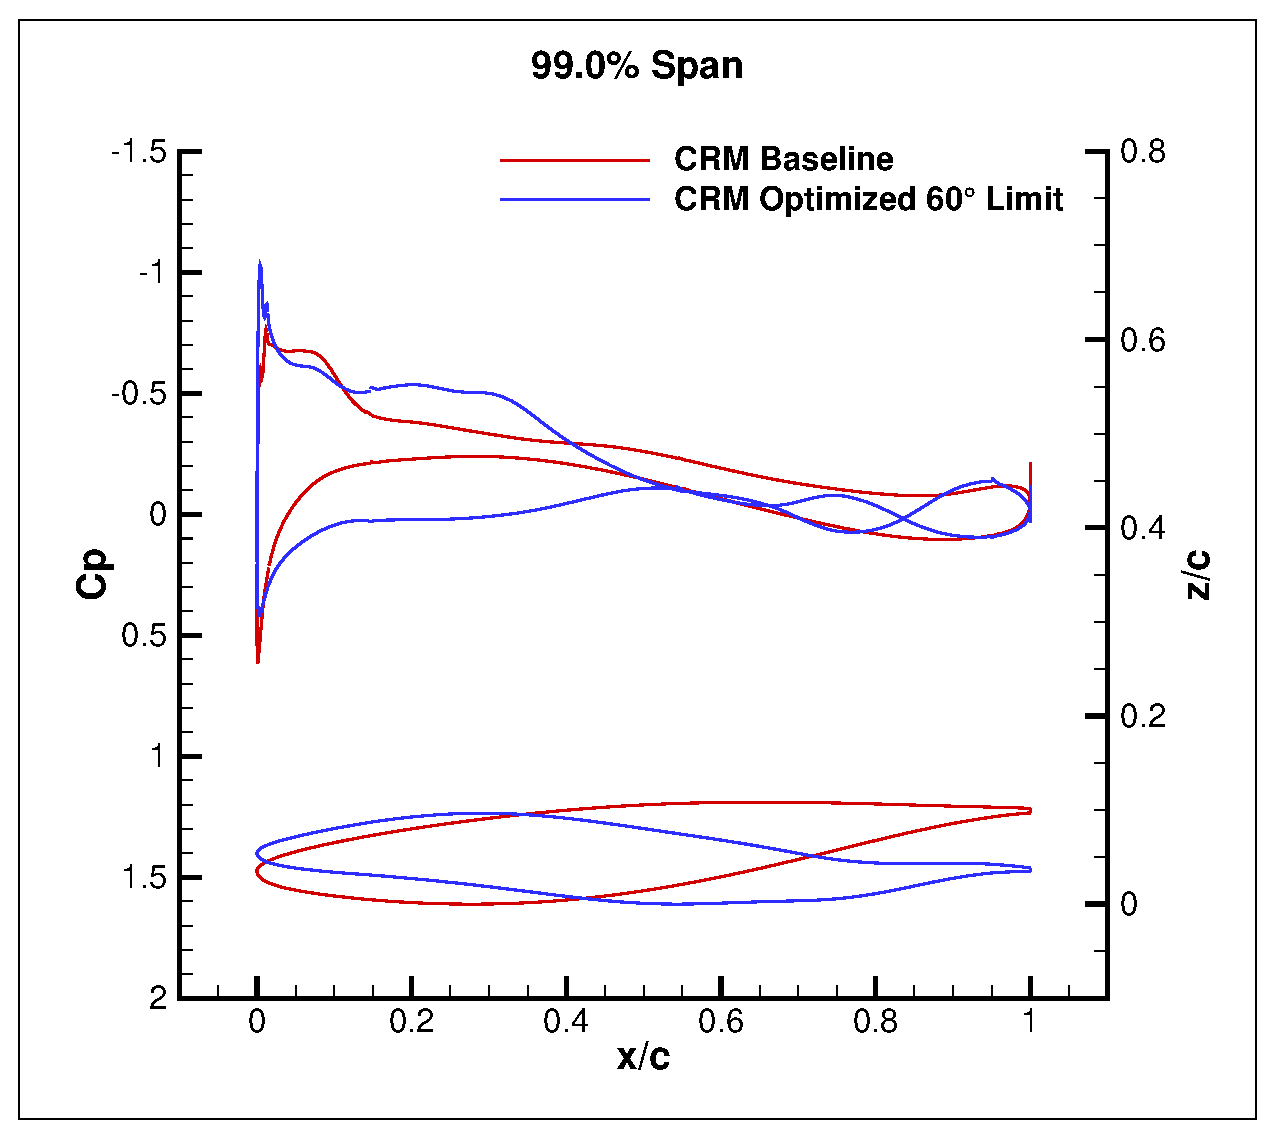
\includegraphics[trim={0.25cm 0.25cm 0.25cm 0.25cm},clip,width=3in]{Figures/With_Twist/CRM/NASA_CRM_Optimize_60deg-99.0percent_Span.eps}}
    \caption{Section geometry and pressure distribution plots of the trimmed angle of attack NASA CRM baseline planform and 60.0\degree\ sweep angle limit optimized planform at 1.00\% (\ref{fig:crm_section_1_perc}), 20.6\% (\ref{fig:crm_section_20.6_perc}), 40.2\% (\ref{fig:crm_section_40.2_perc}), 59.8\% (\ref{fig:crm_section_59.8_perc}), 79.4\%(\ref{fig:crm_section_79.4_perc}), and 99.0\% (\ref{fig:crm_section_99.0_perc}) span.}
\label{fig:crm_section_plots}
\end{figure}
\FloatBarrier

The original geometry exhibits a shock along the entire span of the wing, as evidenced by the close clustering of pressure contour lines towards the trailing edge in Figure~\ref{fig:crm_baseline_planform}, and the sharp drop in pressure that occurs between 60-80\% of the local chord on the upper surface of the wing in Figure~\ref{fig:crm_section_plots}. The optimized geometry resulting from the 60.0\degree\ sweep angle limit is able to completely remove this shock. Furthermore, with the exception of the root and wingtip, the optimizer is able to produce a smooth pressure recovery over the wing, as seen in Figures~\ref{fig:crm_section_20.6_perc}-\ref{fig:crm_section_79.4_perc}. This is also seen in the planform contour plot in Figure~\ref{fig:crm_60_deg_planform}, where the optimized planform displays a more equal spacing between contour lines compared to the trimmed baseline contour plot.

The section shape of the optimized wing differs dramatically from the baseline geometry. The thickness is reduced along the entire span, which differs from other studies. However, this is expected as the CRM optimization case defined in this study does not include a volume constraint, which is contrary to the definitions outlined by the ADODG case. Such a constraint would require the optimizer to redistribute the wing volume to the root~\cite{koo_investigation_2018}. The negative camber towards the root of the wing is reduced in magnitude, with the section becoming increasingly symmetric. Meanwhile, the camber is reduced from 20.6\% span and outboard, with the exception of the wingtip. Furthermore, the negative wing twist is reduced from mid-span and outboard. These camber and wing twist results disagree with the results obtained by by Koo and Zingg~\cite{koo_investigation_2018}, but agree with the results obtained by Lyu et al. and Kenway et al.~\cite{lyu_aerodynamic_2015, kenway_multipoint_2015}—although all three made use of a volume constraint. 
Strange behaviour occurs towards the wingtip. As seen in Figure~\ref{fig:crm_section_99.0_perc}, the leading half of the wing exhibits a negative twist, whereas the trailing half of the wing appears to be at a similar twist relative to the section at 79.4\% span in Figure~\ref{fig:crm_section_79.4_perc}. The overall twist at 99.0\% span appears to be a substantial reduction compared to the original geometry, but it is unclear why this result has occurred. This behaviour is unique to this study and does not appear in previous aerodynamic shape optimizations on the NASA CRM wing~\cite{koo_investigation_2018, shi-dong_adjoint-based_2017, lyu_aerodynamic_2015, kenway_multipoint_2015}. It must be noted that the spanwise sections used for measurement in this study differ from those specified in ADODG Case 4 and reported in other studies~\cite{martins_aerodynamic_2022, koo_investigation_2018, shi-dong_adjoint-based_2017, lyu_aerodynamic_2015, kenway_multipoint_2015}, such that the root and wingtip sections measured in this study are not the same as those used in ADODG Case 4. The section measured closest to the root is at 1.00\% span in this study whereas ADODG Case 4 reports measurements at 2.35\%. Similarly, section closest to the wingtip in this study occurs at 99.0\% span, whereas the measurement is taken at 94.4\% span in ADODG Case 4.. It is possible that analysis of the sections using the spanwise points dictated by ADODG Case 4 may show that such artifacts do not occur at its outermost measurement section at 94.4\% span. Nevertheless, the overall increase in twist from 20.6\% span to the wingtip disagrees with the results obtained by Koo and Zingg~\cite{koo_investigation_2018}, but closely agrees with the results obtained by Lyu et al. and Kenway et al.~\cite{lyu_aerodynamic_2015, kenway_multipoint_2015}, with the exception of the section shape at the wingtip. All three studies present slight variations on ADODG case 4 with respect to their optimization constraints, such that all three studies produce slightly different results. Nevertheless, the changes in camber and thickness found in this study—with the exception of the root due to this study's exclusion of a volume constraint—otherwise match all three of the aforementioned studies' results.

%%%%%%%%%%%%%%%%%% TALK ABOUT WEIRD TWIST BEHAVIOUR HERE %%%%%%%%%%%%%%%%%%
The wing twist artifact occurring at 99.0\% span seen in Figure~\ref{fig:crm_section_99.0_perc} was of particular concern. Its varying twist along the chord does not agree with other studies, wherein such phenomena did not arise~\cite{koo_investigation_2018, lyu_aerodynamic_2015, kenway_multipoint_2015}. Analysis of the outboard sections of the 60.0\degree\ limit optimized geometry illustrated significant oscillations in wing twist, as seen in Figure~\ref{fig:crm_artifacts}. An additional optimization was conducted with a 45.0\degree\ upper sweep angle limit to observe if this behaviour occurs at lower sweep angles as well. Indeed, oscillations of similar magnitude occur at the trailing edge with a 45.0\degree sweep angle as well, as seen in Figure~\ref{fig:crm_artifacts_45deg}. This behaviour is not desirable, as it is not manufacturable within the context of conventional aircraft design. Therefore, an additional study was run on the NASA CRM with an otherwise identical methodology, with the exception of wing twist as a design variable and the selection of sweep angle limits, which are outlined in the following section.
% Also include images
\begin{figure}[!tp]
    \centering
    \subfloat[\label{fig:crm_artifact_01}]{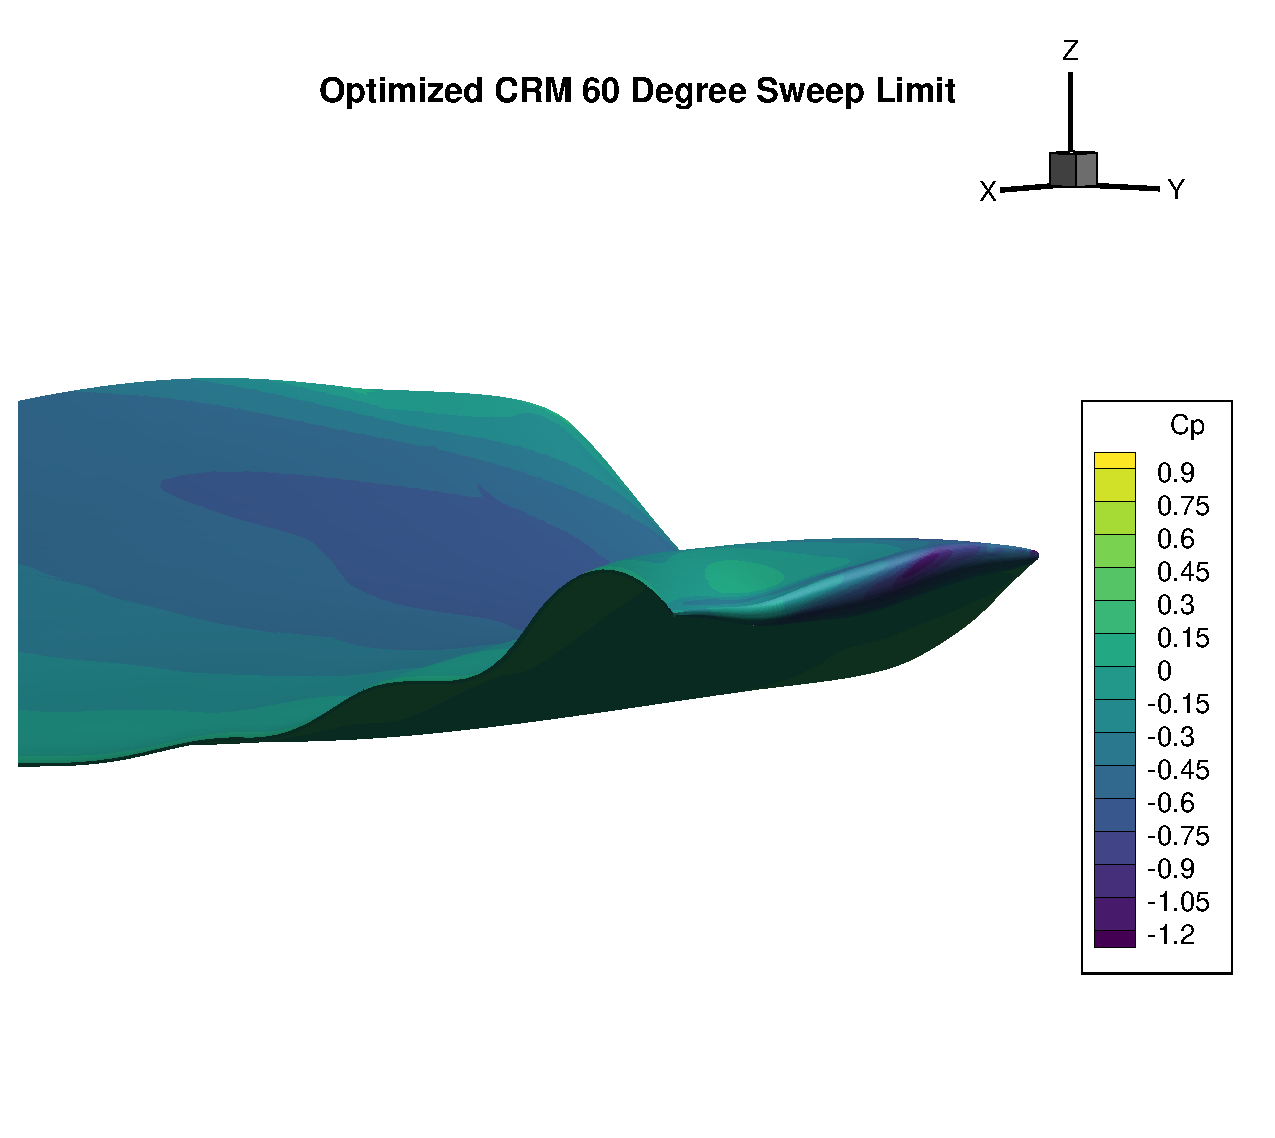
\includegraphics[trim={0.25cm 0.25cm 0.25cm 0.25cm},clip,width=3.175in]{Figures/With_Twist/CRM/Optimize_CRM_60deg_Twist_Artifact_01.eps}}
    \hspace{0.25cm}
    \subfloat[\label{fig:crm_artifact_02}]{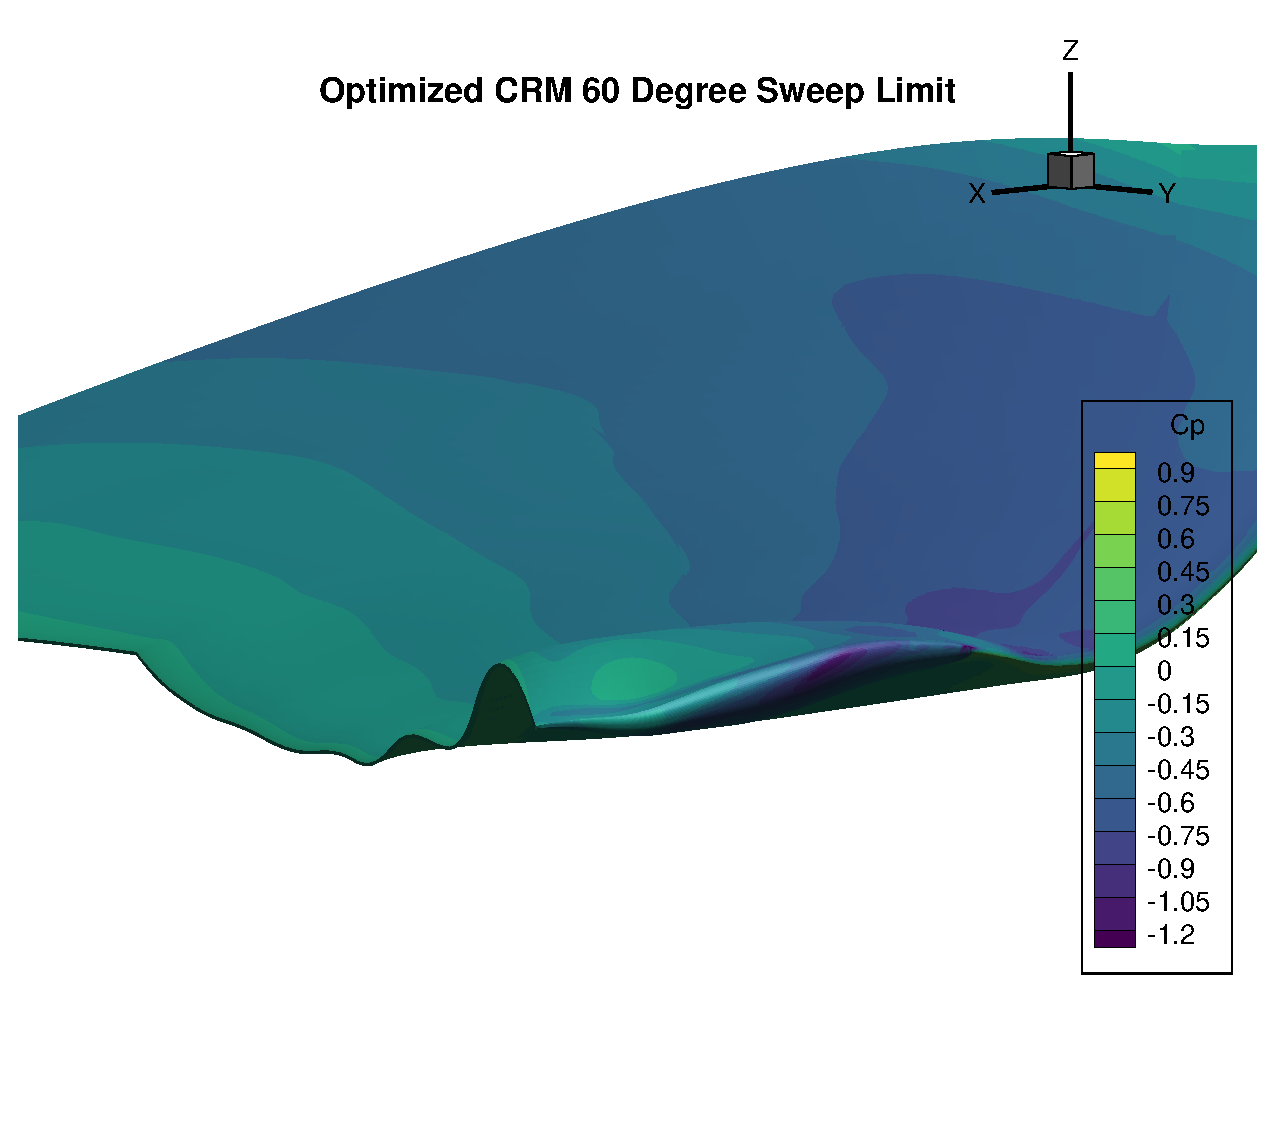
\includegraphics[trim={0.25cm 0.25cm 0.25cm 0.25cm},clip,width=3.175in]{Figures/With_Twist/CRM/Optimize_CRM_60deg_Twist_Artifact_02.eps}}
    \caption{Trailing edge geometry artifacts observed in the CRM 60.0\degree\ sweep angle limit optimized planform.}
\label{fig:crm_artifacts}
\end{figure}

\begin{figure}[!tp]
\centering
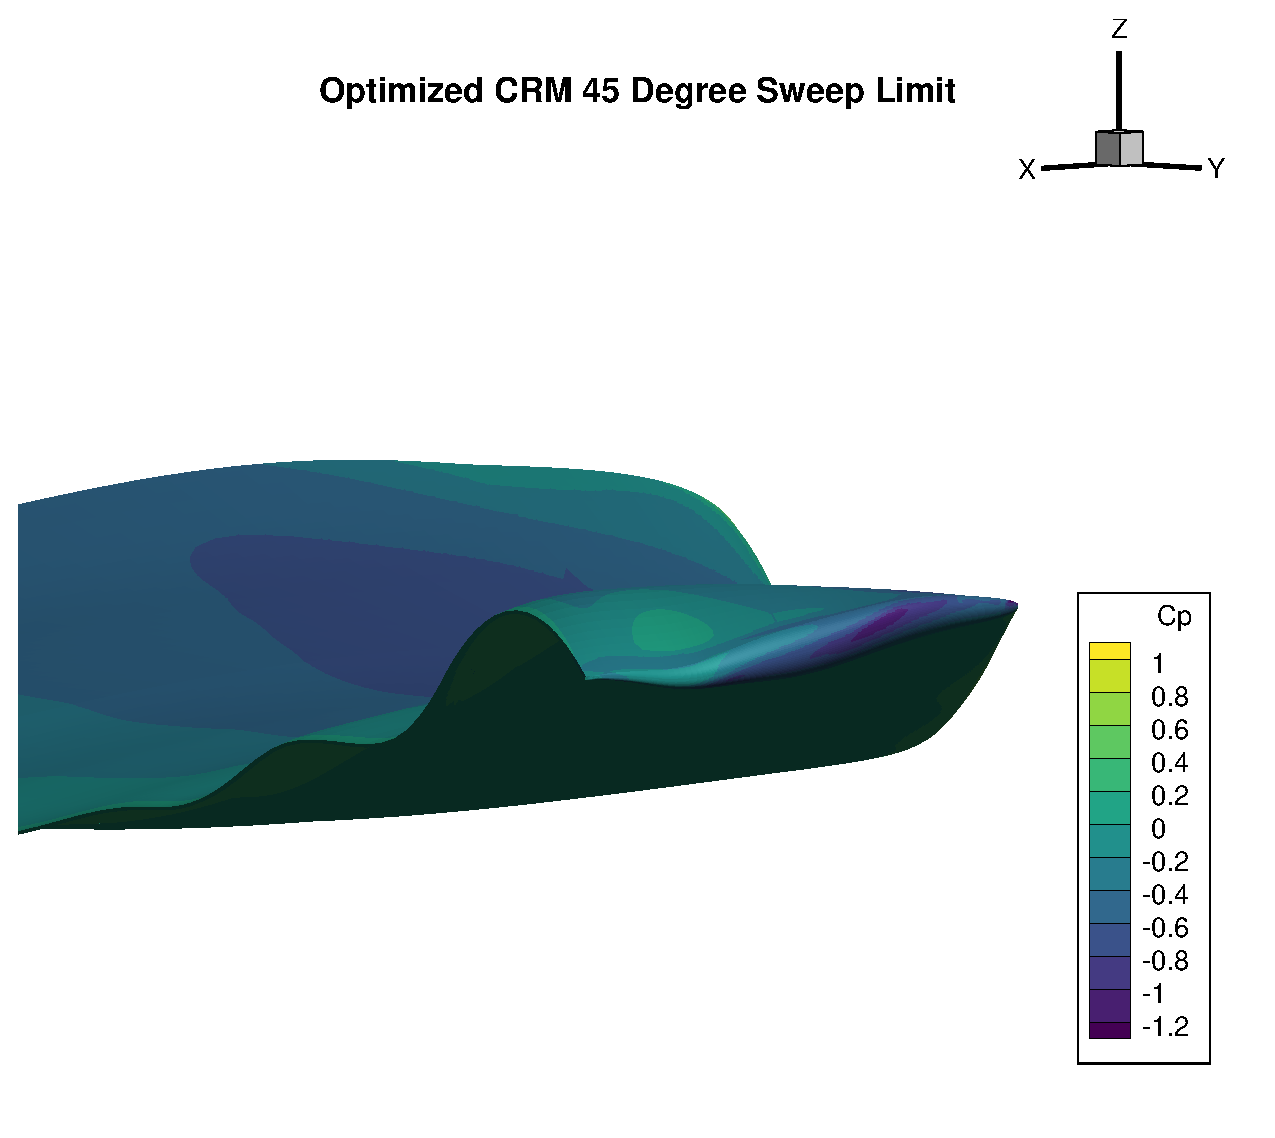
\includegraphics[width=4.5in]{Figures/With_Twist/CRM/Optimize_CRM_45deg_Twist_Artifact_01.eps}
\caption{Trailing edge geometry artifacts observed in a CRM 45.0\degree\ sweep angle limit optimized planform.}
\label{fig:crm_artifacts_45deg}
\end{figure}
%%%%%%%%%%%%%%%%%% INTRODUCE NEW CASE WITHOUT TWIST %%%%%%%%%%%%%%%%%%
\subsection{NASA CRM Optimization without Wing Twist}
\label{ssec:crm-opt-notwist}
In light of the geometry artifacts associated with wing twist on the NASA CRM wing, a second study was performed without wing twist as a design variable. The second case was run with an equality constraint on the wing twist set to 0\degree. Owing to the knowledge of optimization behaviour obtained in the initial CRM ASO study, the sweep angle was immediately expanded to 60.0\degree.

Furthermore, considering the substantial drag improvements obtained in the initial study on the CRM, ASO without wing twist was conducted on the NASA CRM at its original sweep angle of 37.5\degree\ as well. This result served to place the 60.0\degree\ sweep angle limit result without wing twist into context, as an optimization of the CRM at the original wing sweep angle is likely to be a more common method of optimizing a wing, as evidenced by many modern ASO studies~\cite{lyu_rans-based_2014, lyu_aerodynamic_2015, osusky_drag_2015, streuber_investigation_2017, koo_investigation_2018}. Therefore, the result obtained from this optimization was considered to be the benchmark over which the sweep-inclusive optimization must display a tangible benefit in order to be valuable.

%%%%%%%%% CRM WITHOUT TWIST RESULTS %%%%%%%%%%%
The CRM ASO with a fixed sweep angle matching the original sweep angle of 37.5\degree\ progressed very smoothly, with analysis of the merit function, optimality, and feasibility of this study illustrating that this case was converged after 267 design iterations, as seen in Figure~\ref{fig:crm_notwist_converge_optimized_baseline}. The drag coefficient $C_D S$ had decreased by 52.7 drag counts, with a small decrease in angle of attack, as seen in Table~\ref{tab:crm_notwist_results}. The $L/D$ increased by over 2.8 from 28.78 to 31.59. This performance is slightly better than that that obtained in the 45.9\degree\ case with wing twist in the initial study, but it must be noted that this case was not converged.

The CRM ASO with a sweep angle limit of 60.0\degree\ observed smooth convergence as well. Analysis of the merit function, optimality, and feasibility of this study indicated that this study had converged after 259 design iterations, as seen in Figure~\ref{fig:crm_notwist_converge_60.0_deg}. The drag coefficient, $C_D S$, had decreased by 58.8 drag counts relative to the trimmed baseline wing, with a small decrease in angle of attack, as seen in Table~\ref{tab:crm_notwist_results}. The moment coefficient, $C_M S$, decreased substantially from -2.704 to -3.742. The $L/D$ increased by over 3.1 from 28.78 to 31.59. This performance is an improvement by 1.14\% over the optimized CRM at the original sweep angle of 37.5\degree; however, the 60.0\degree\ case with twist included remains 0.43\% better than the 60.0\degree\ case without twist, with lower drag by 2.3 drag counts. Nonetheless, its geometry artifacts prevent it from being a legitimate comparison due to the unrealistic manufacturing requirements that would result. Therefore, the results without wing twist serve as this study's primary basis for wing sweep performance comparisons on the NASA CRM wing.

Plots of the upper surface pressure contours on the optimized planforms for the ASOs at the original sweep angle of 37.5\degree\ and the 60.0\degree\ sweep angle limit cases are shown in Figure~\ref{fig:crm_notwist_planform_plots}. Plots of the section geometry and pressure distribution at various spanwise sections for the trimmed angle of attack baseline, the fixed-sweep ASO at the original sweep angle of 37.5\degree, and the 60.0\degree\ sweep angle limit ASO cases are given in Figure~\ref{fig:crm_notwist_section_plots}.

\begin{table}[!tp]
\centering
\caption{Results summary for the optimization of the NASA CRM without wing twist}
\label{tab:crm_notwist_results}
\begin{adjustbox}{center}
\begin{tabular}{lcccc}
\hline\hline
Design Variable & Trimmed Baseline & Original (37.5\degree)\ Sweep Limit & 60.0\degree\ Sweep Limit\\
\hline
$S$ (ref. units\textsuperscript{2}) & 3.395 & 3.394 & 3.393\\
$C_L S$ & 1.6972 & 1.6972 & 1.6972\\
$C_M S$ & -2.704 & -2.717 & -3.742 \\
$C_D S$ (counts) & 589.7 & 537.2 & 531.1\\
$L/D$ & 28.78 & 31.59 & 31.96\\
Angle of Attack & 1.982\degree\ & 1.771\degree\ & 2.225\degree\ \\
\makecell[l]{Post-Optimization\\Leading Edge Sweep Angle} & 37.50\degree\ & 37.31\degree\ & 48.50\degree\ \\
\hline\hline
\end{tabular}
\end{adjustbox}
\end{table}
% images
%%%%%%%%% CRM WITHOUT TWIST CONVERGENCE HISTORY %%%%%%%%%%%
\begin{figure}[!tp]
\centering
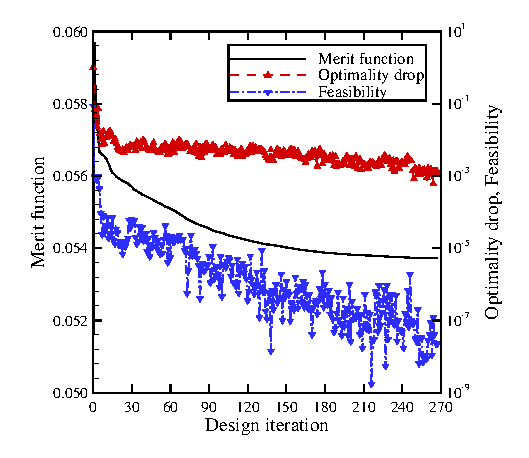
\includegraphics[width=4.5in]{Figures/No_Twist/NASA_CRM/Optimize_CRM_FIXED_Orig_No_Twist.eps}
\caption{Convergence history for NASA-CRM optimization without wing twist and a sweep angle limit at the original sweep angle of 37.5\degree.}
\label{fig:crm_notwist_converge_optimized_baseline}
\end{figure}

\begin{figure}[!tp]
\centering
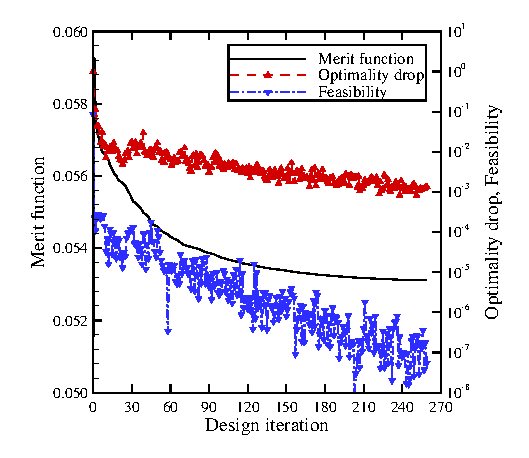
\includegraphics[width=4.5in]{Figures/No_Twist/NASA_CRM/Optimize_CRM_No_Twist_60deg.eps}
\caption{Convergence history for NASA-CRM optimization without wing twist and an upper sweep angle limit of 60.0\degree.}
\label{fig:crm_notwist_converge_60.0_deg}
\end{figure}

%%%%%%%%% CRM WITHOUT TWIST UPPER CP CONTOURS %%%%%%%%%%%
\begin{figure}[!tp]
    \centering
    %%%%%% Decided not to include original CRM again %%%%%%
    % \subfloat[\label{fig:crm_notwist_baseline_planform}]{\includegraphics[trim={0.25cm 0.25cm 0.25cm 0.25cm},clip,width=3.175in]{Figures/No_Twist/NASA_CRM/NASA_CRM_Baseline_Trimmed-Contour-Upper.eps}}\\
    \subfloat[\label{fig:crm_notwist_optimized_baseline_planform}]{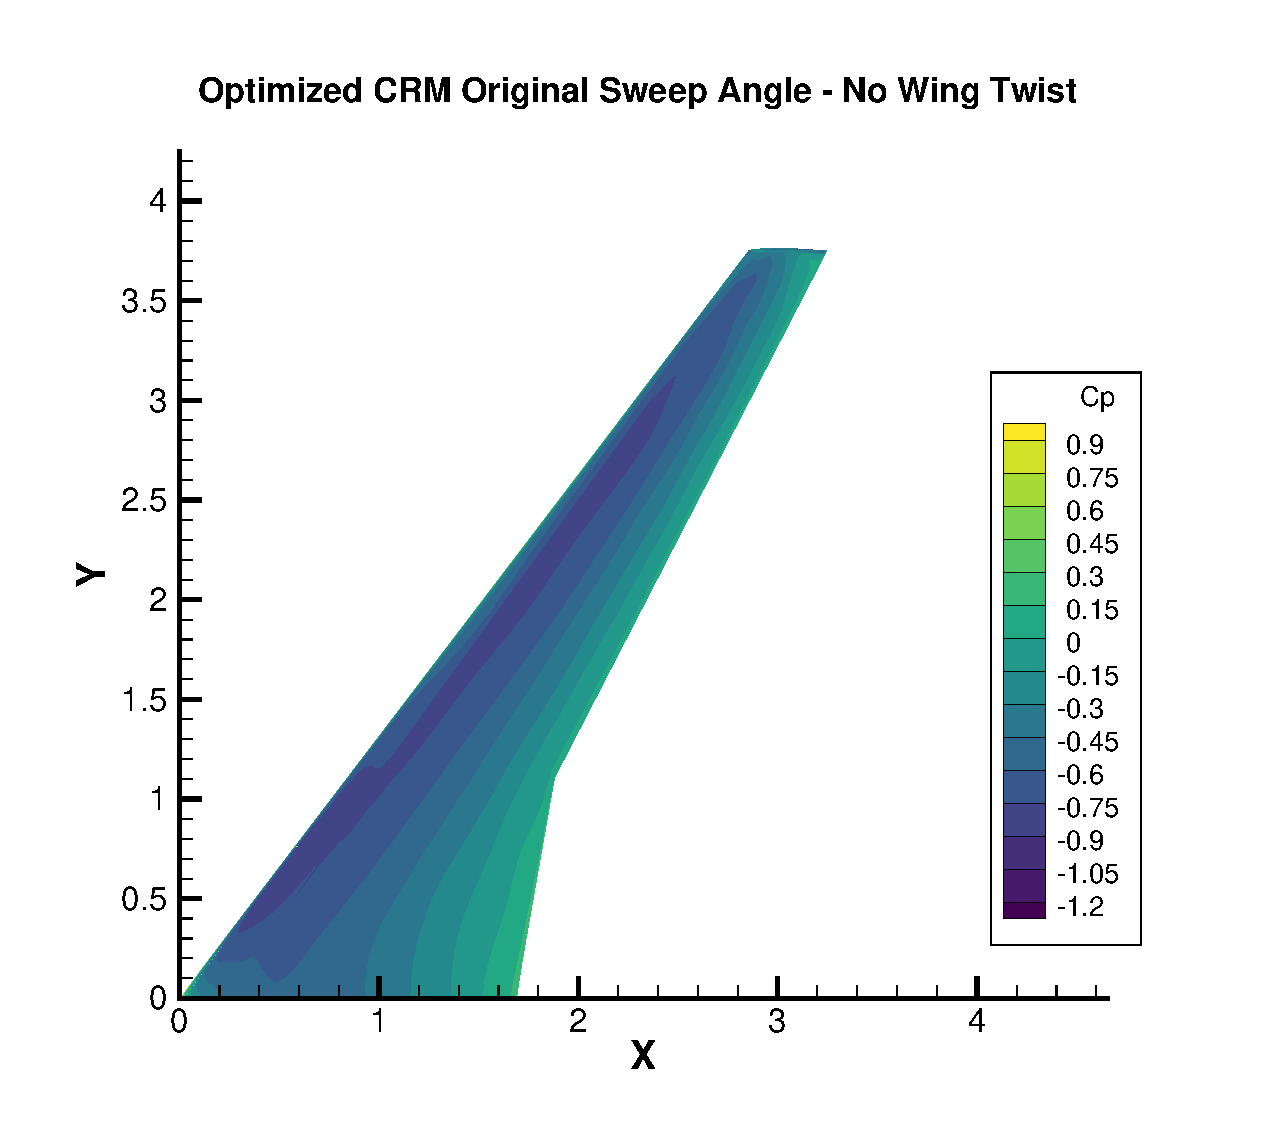
\includegraphics[trim={0.25cm 0.25cm 0.25cm 0.25cm},clip,width=3.175in]{Figures/No_Twist/NASA_CRM/NASA_CRM_FIXED_Orig_NoTwist-Contour-Upper.eps}}
    \hspace{0.25cm}
    \subfloat[\label{fig:crm_notwist_60_deg_planform}]{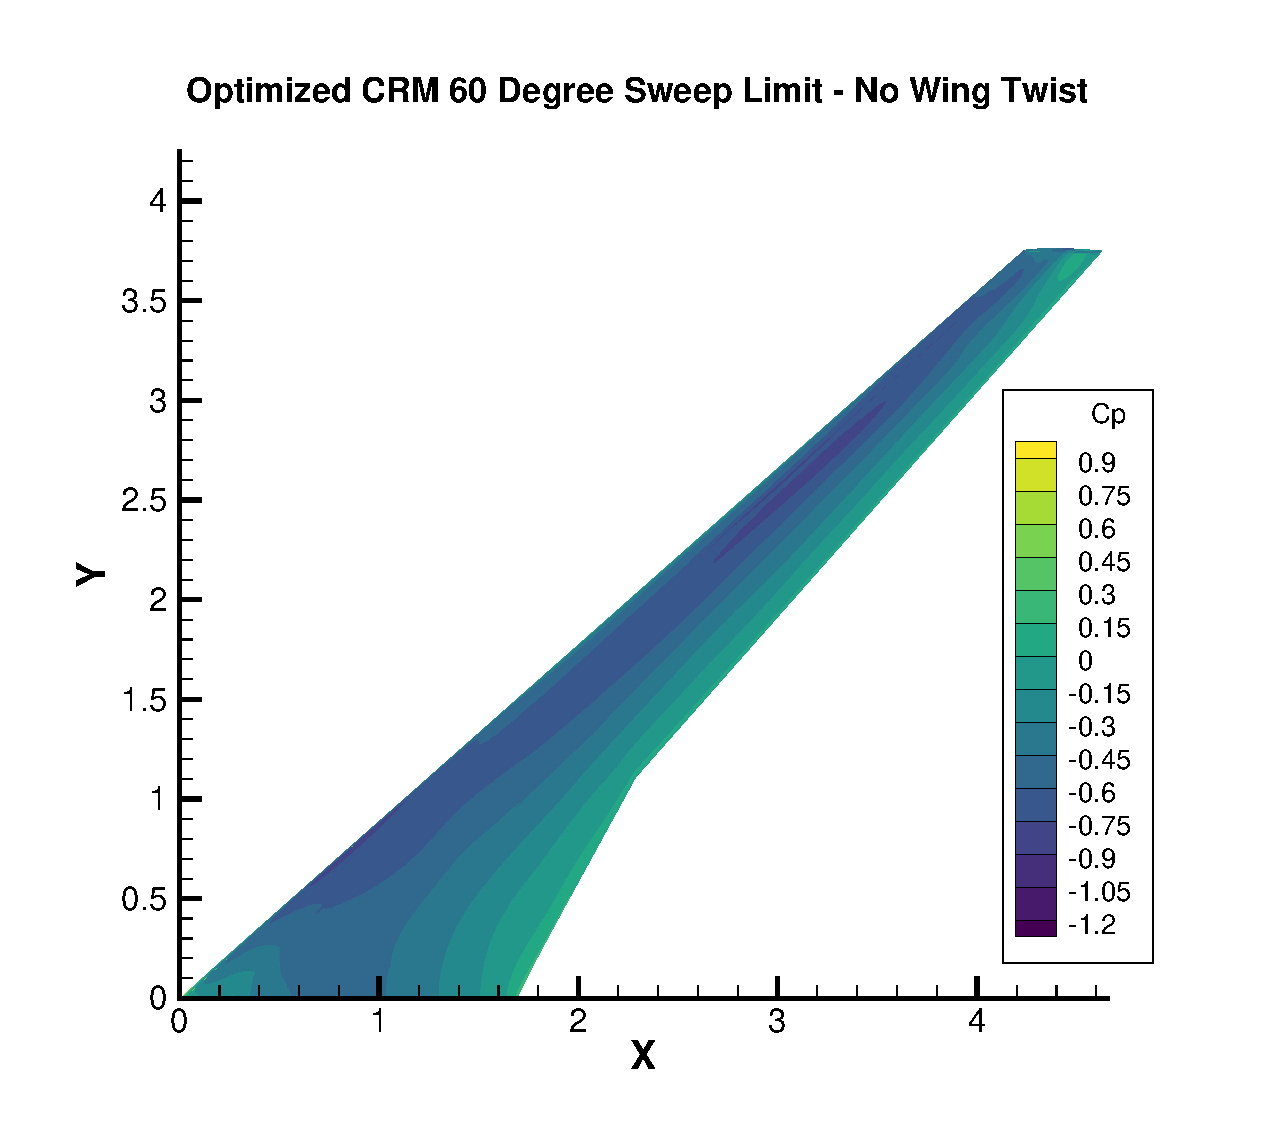
\includegraphics[trim={0.25cm 0.25cm 0.25cm 0.25cm},clip,width=3.175in]{Figures/No_Twist/NASA_CRM/NASA_CRM_varsweep_60deg_NoTwist-Contour-Upper.eps}}
    \caption{Upper surface pressure contours for the original sweep angle limit optimized planform (\ref{fig:crm_notwist_optimized_baseline_planform}) and the 60.0\degree\ sweep angle limit optimized planform (\ref{fig:crm_60_deg_planform}) without wing twist in optimization.}
\label{fig:crm_notwist_planform_plots}
\end{figure}

%%%%%%%%%% CRM WITHOUT TWIST SECTION SHAPES %%%%%%%%%%%
\begin{figure}[!tp]
    \centering
    \subfloat[\label{fig:crm_notwist_section_1_perc}]{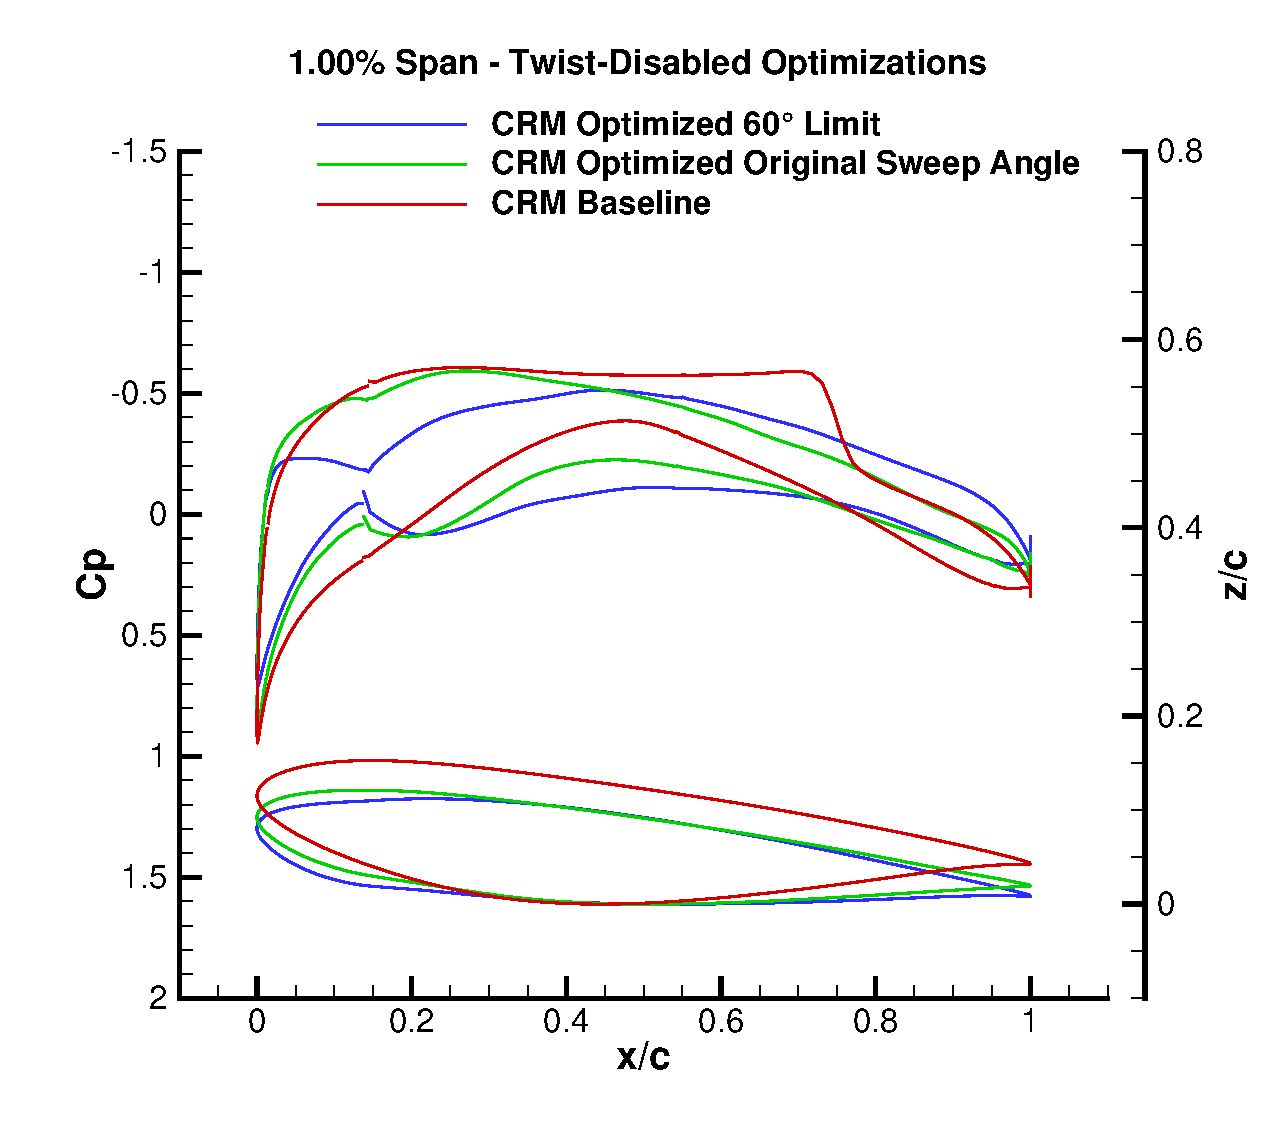
\includegraphics[trim={0.2cm 0.2cm 0.2cm 0.2cm},clip,width=3in]{Figures/No_Twist/NASA_CRM/NASA_CRM_Optimize_NoTwist-1.00percent_Span.eps}}
    \hspace{0.2cm}
    \subfloat[\label{fig:crm_notwist_section_20.6_perc}]{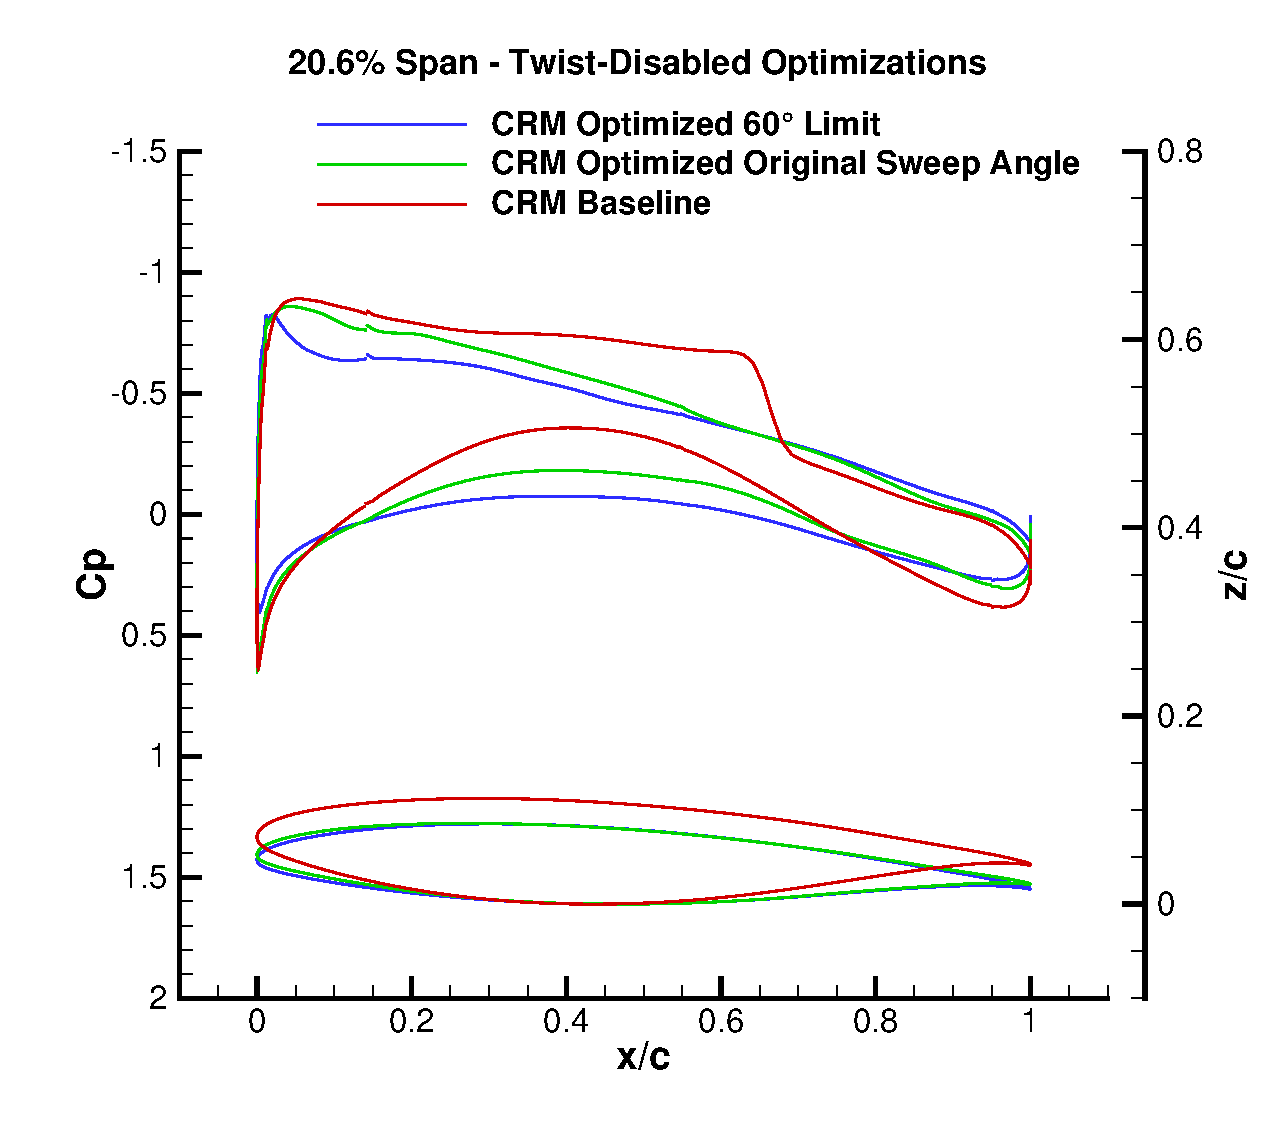
\includegraphics[trim={0.2cm 0.2cm 0.2cm 0.2cm},clip,width=3in]{Figures/No_Twist/NASA_CRM/NASA_CRM_Optimize_NoTwist-20.6percent_Span.eps}}\\
    \subfloat[\label{fig:crm_notwist_section_40.2_perc}]{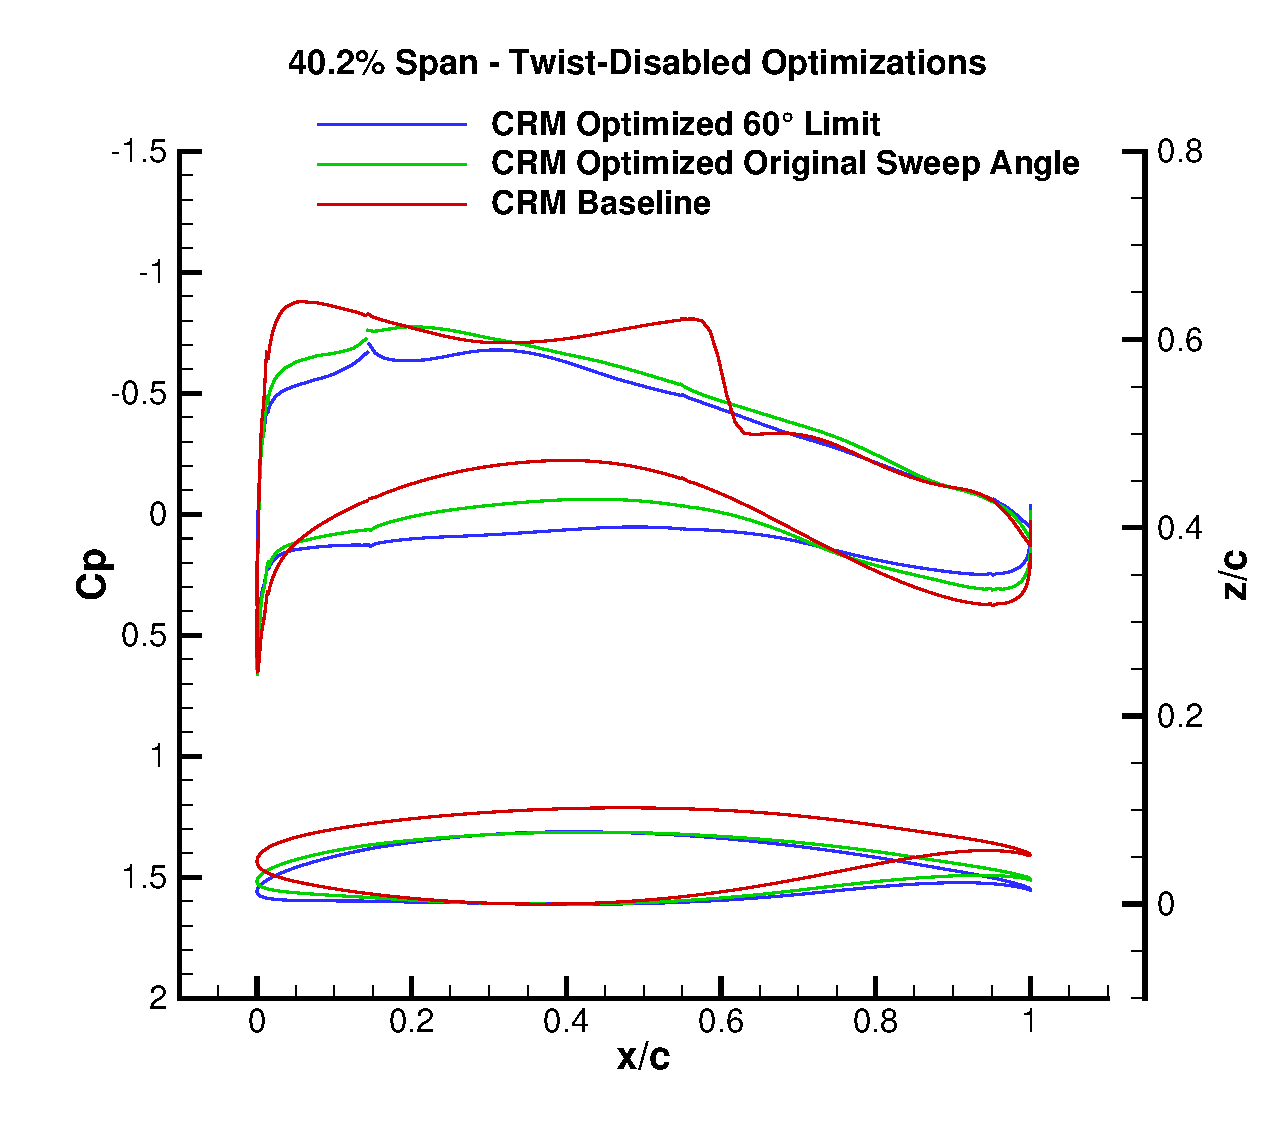
\includegraphics[trim={0.2cm 0.2cm 0.2cm 0.2cm},clip,width=3in]{Figures/No_Twist/NASA_CRM/NASA_CRM_Optimize_NoTwist-40.2percent_Span.eps}}
    \hspace{0.2cm}
    \subfloat[\label{fig:crm_notwist_section_59.8_perc}]{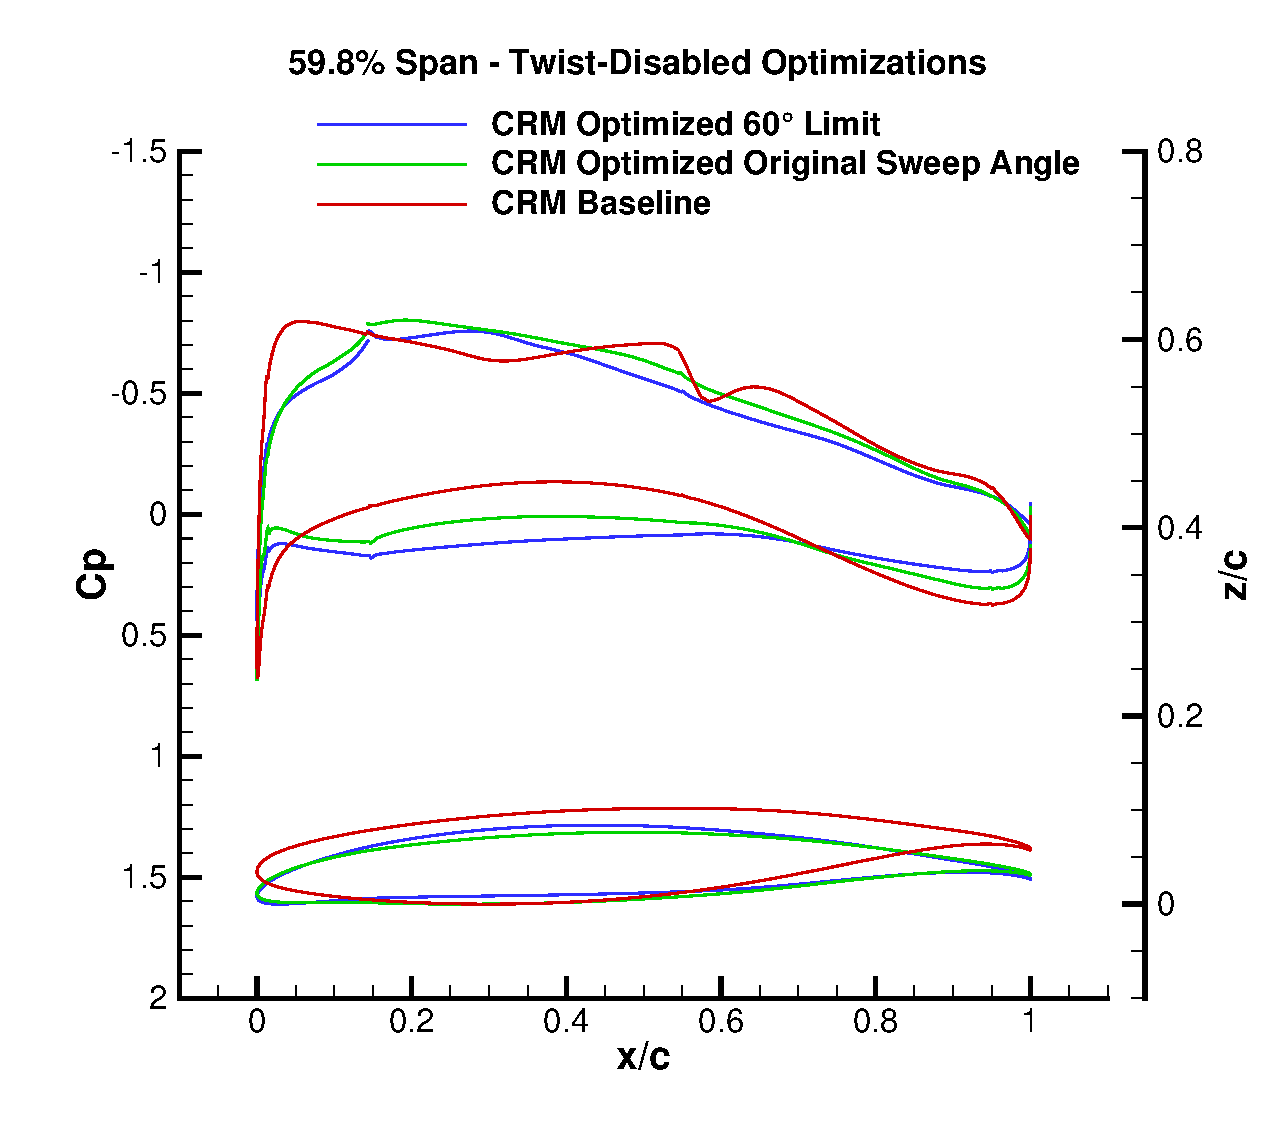
\includegraphics[trim={0.2cm 0.2cm 0.2cm 0.2cm},clip,width=3in]{Figures/No_Twist/NASA_CRM/NASA_CRM_Optimize_NoTwist-59.8percent_Span.eps}}\\
    \subfloat[\label{fig:crm_notwist_section_79.4_perc}]{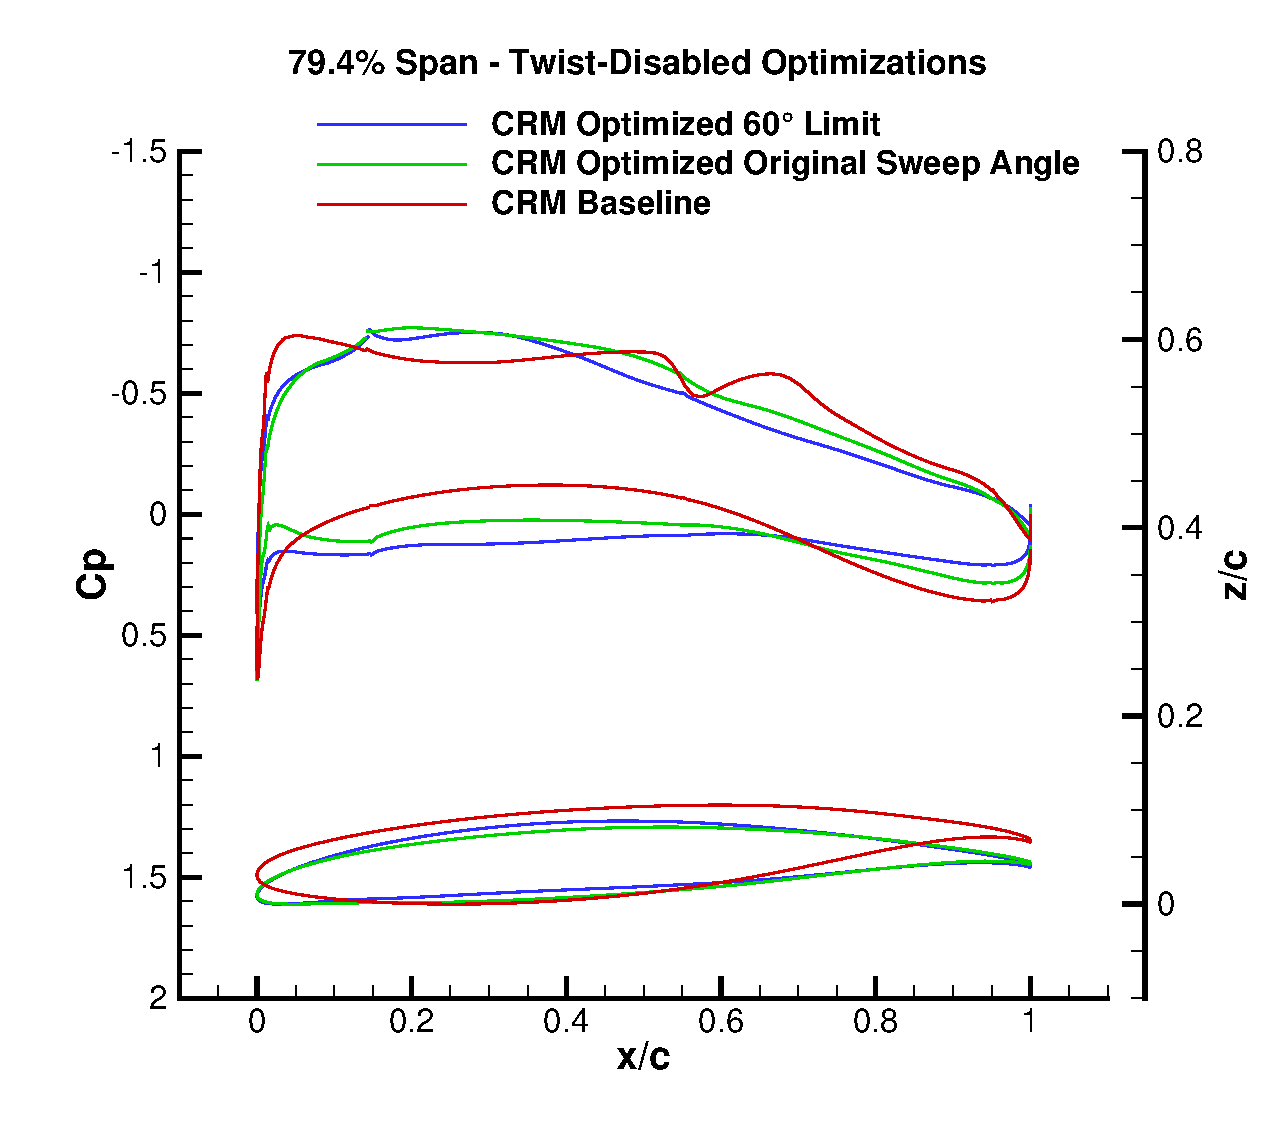
\includegraphics[trim={0.2cm 0.2cm 0.2cm 0.2cm},clip,width=3in]{Figures/No_Twist/NASA_CRM/NASA_CRM_Optimize_NoTwist-79.4percent_Span.eps}}
    \hspace{0.2cm}
    \subfloat[\label{fig:crm_notwist_section_99.0_perc}]{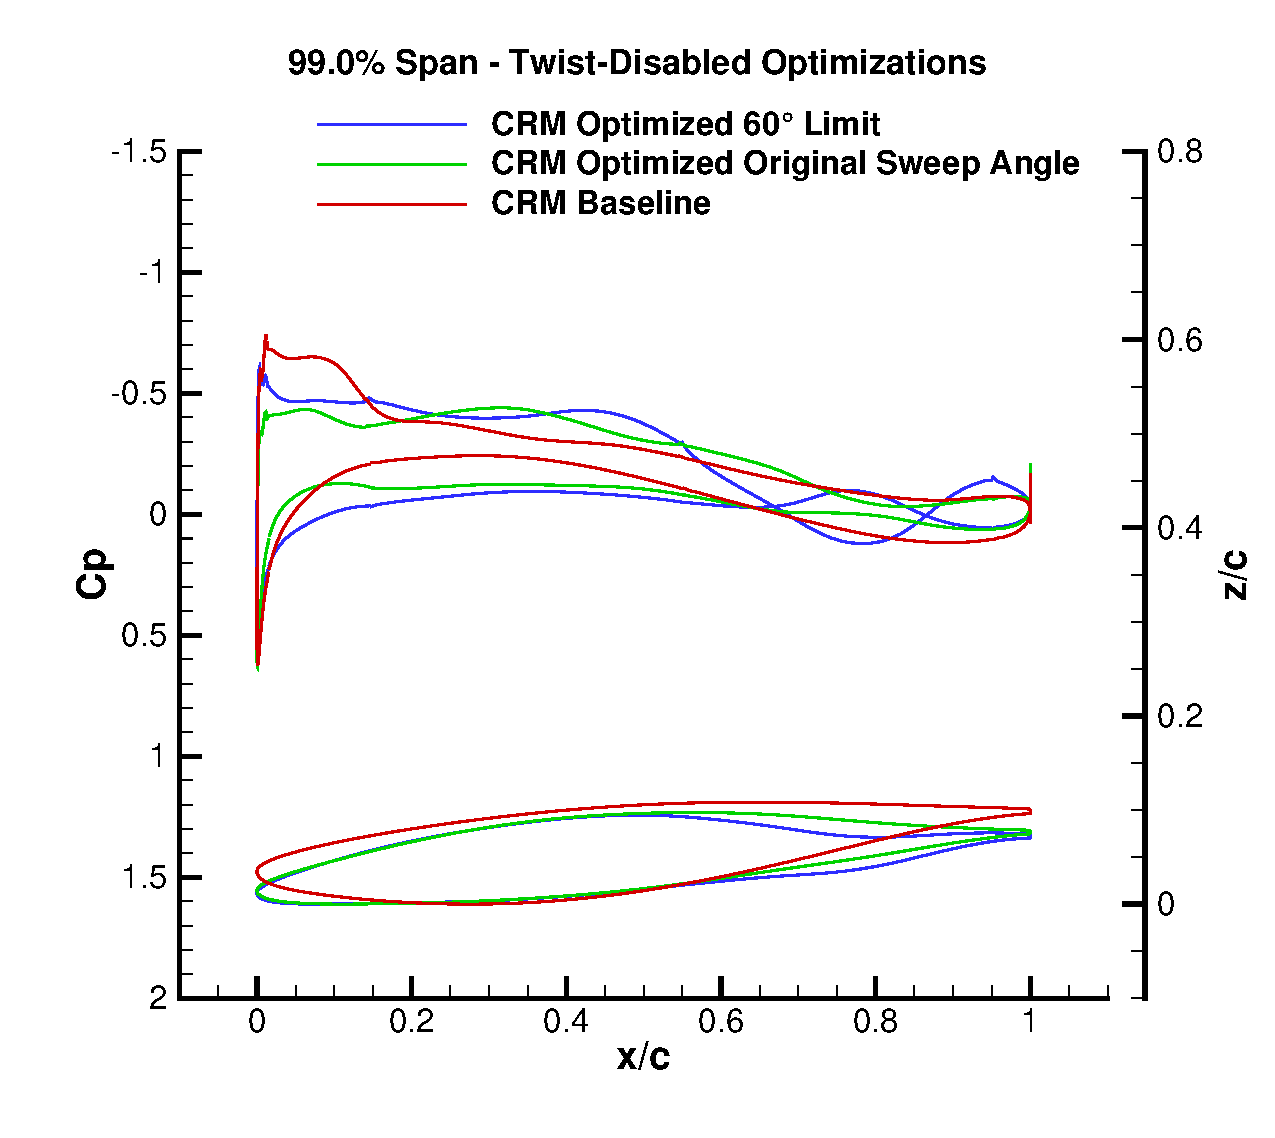
\includegraphics[trim={0.2cm 0.2cm 0.2cm 0.2cm},clip,width=3in]{Figures/No_Twist/NASA_CRM/NASA_CRM_Optimize_NoTwist-99.0percent_Span.eps}}
    \caption{Section geometry and pressure distribution plots of the trimmed angle of attack NASA CRM baseline planform, original sweep angle limit optimized planform, and 60.0\degree\ sweep angle limit optimized planform wihout wing twist in optimization at 1.00\% (\ref{fig:crm_notwist_section_1_perc}), 20.6\% (\ref{fig:crm_notwist_section_20.6_perc}), 40.2\% (\ref{fig:crm_notwist_section_40.2_perc}), 59.8\% (\ref{fig:crm_notwist_section_59.8_perc}), 79.4\%(\ref{fig:crm_notwist_section_79.4_perc}), and 99.0\% (\ref{fig:crm_notwist_section_99.0_perc}) span.}
\label{fig:crm_notwist_section_plots}
\end{figure}
\FloatBarrier

Compared to the trimmed baseline in Figure~\ref{fig:crm_baseline_planform}, the shock that occurs 60-80\% of the local chord on the upper surface of the wing in Figure~\ref{fig:crm_notwist_section_plots} is eliminated on both optimized planforms.
% Remove unnecessary detail
% As stated previously, the original geometry exhibits close clustering of pressure contour lines towards the trailing edge and a sharp drop in pressure that occurs between 60-80\% of the local chord on the upper surface of the wing in Figure~\ref{fig:crm_section_plots}, which is indicative of a shock along the entire span of the wing. Meanwhile, the absence of such characteristics on both optimized planforms indicates that both geometries are able to eliminate the shock wave, implying that wave drag is also substantially reduced or completely eliminated. Indeed, inspection of the section shape plots in Figure~\ref{fig:crm_notwist_section_plots} shows that the 60.0\degree\ sweep angle limit case is able to completely eliminate shocks over its entire span, as the pressure recovery is very smooth on the inboard sections of the wing. Strange behaviour is observed near the root for the 60.0\degree\ sweep angle limit case, where a cusp occurs on both the upper and lower surfaces. The source of this behaviour was unclear.
Notably, the optimization at the fixed sweep angle of 37.5\degree\ exemplifies a substantial improvement in shock characteristics over the trimmed baseline geometry without any changes to the wing sweep angle. One observes that that with the exception of the outboard sections of the wing, the pressure recovery is almost as smooth as that obtained in the 60.0\degree\ sweep angle limit case.
% In fact, it appears that this case is able to remove the shock waves as well.
% Minor perturbations exist during the pressure recovery at 79.4\% span as seen in Figure~\ref{fig:crm_notwist_section_79.4_perc}, but it is unclear why this has occurred. 

The section shapes for both the 37.5\degree\ fixed sweep angle and 60.0\degree\ sweep angle limit optimizations appear quite similar, with the 60.0\degree\ sweep angle limit simply appearing as a more exaggerated version of the former. 
% The negative camber towards the root is reduced in magnitude, which is similar to the 60.0\degree\ sweep angle limit case with wing twist. The camber is similarly reduced at 20.6\% span as well. Some differences to the twist-inclusive results appear in both the 37.5\degree\ fixed sweep angle and 60.0\degree\ sweep angle limit cases at 40.2\% span, where both cases have made the airfoil substantially thinner, as seen in Figure~\ref{fig:crm_notwist_section_40.2_perc}.
Changes to the airfoil's camber are complex—the airfoil reflex has been eliminated and the lower section flattened out. Meanwhile, the leading edge of the airfoil has lowered substantially, which maintains positive camber in the section shape despite the flattened lower section. Similar behaviour appears at 59.8\% and 79.4\% span in both twist-deactivated cases, as seen in Figures~\ref{fig:crm_notwist_section_59.8_perc} and~\ref{fig:crm_notwist_section_79.4_perc}. This lowering of the leading edge while flattening the lower section appears to be an attempt to modify the local twist on the wing without violating the the twist equality constraint of 0\degree. Indeed, converting the reflexed camber line to a positive camber line with a lowered leading edge visually appears to have this effect, showing that the optimizer is more than capable of exploiting the freedom given to it. 

The pressure coefficient behaviour and section shape results at the wingtip remain complex. Just as in the 60.0\degree\ sweep case with twist, odd changes to the airfoil have occurred along its entire length, seen in Figure~\ref{fig:crm_notwist_section_99.0_perc}.
% A reflexed camber line has been generated in the 60.0\degree\ sweep angle limit case without wing twist, with positive camber at the leading edge and negative camber towards the trailing edge, seen in Figure~\ref{fig:crm_notwist_section_99.0_perc}. It appears that the fixed-sweep optimization at 37.5\degree\ exhibits this behaviour as well, although less severely. 
It remains unclear why this behaviour has occurred, although as before, it does not appear in other studies on the CRM wing~\cite{martins_aerodynamic_2022, koo_investigation_2018, shi-dong_adjoint-based_2017, lyu_aerodynamic_2015, kenway_multipoint_2015} and may be attributed to the difference in locations along the wingspan used for plotting the section shape and $C_p$ in this study.

Alignment with the results of other studies is not possible for the optimization cases without wing twist. A search of relevant literature containing studies of the NASA CRM on a similar basis to this study make use of wing twist, including those conducted by by Koo and Zingg, Lyu et al., and Kenway et al.~\cite{koo_investigation_2018, lyu_aerodynamic_2015, kenway_multipoint_2015}, such that the results presented here are novel at the time of writing.

\section{A320neo Optimization}
\subsection{A320neo Optimization with Wing Twist}
\label{ssec:a320neo-opt-twist}
The initial optimization of the A320neo geometry was carried out using the procedure outlined in section~\ref{ssec-prob-formulate}. Similar to the CRM optimizations, the initial choices in the upper wing sweep angle limit proved to be too low. The 45.5\degree sweep limit was expanded to 50.0\degree, and then expanded again to 60.0\degree to ensure a sufficient margin between the resultant wing sweep angle and the upper limit. The convergence history and and results for all three sweep angle limits are provided for completeness, and are presented in Figures~\ref{fig:a320neo_converge_45.5_Deg},~\ref{fig:a320neo_converge_50.0_Deg},~\ref{fig:a320neo_converge_60.0_Deg}, and Table~\ref{tab:a320neo_results}.

% Observation of the design variable history during optimization iterations illustrated that the wing sweep rose to its upper limit of 37.7\degree\ within 60 iterations and remained there. The optimization was manually stopped after 88 design iterations. Analysis of the merit function, optimality, and feasibility of this study illustrated that this case was not converged, as seen in Figure~\ref{fig:a320neo_converge_45.5_Deg}.

\begin{figure}[!tp]
    \centering
    \subfloat[\label{fig:a320neo_converge_45.5_Deg}]{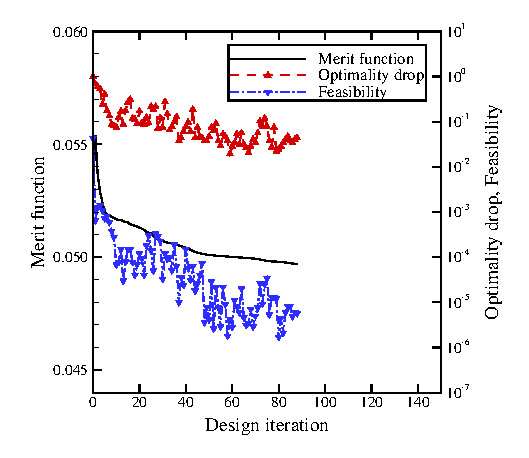
\includegraphics[trim={0.15cm 0cm 0.15cm 0cm},clip,width=3.175in]{Figures/With_Twist/A320neo/optimize_A320neo.eps}}
    \hspace{0.25cm}
    \subfloat[\label{fig:a320neo_converge_50.0_Deg}]{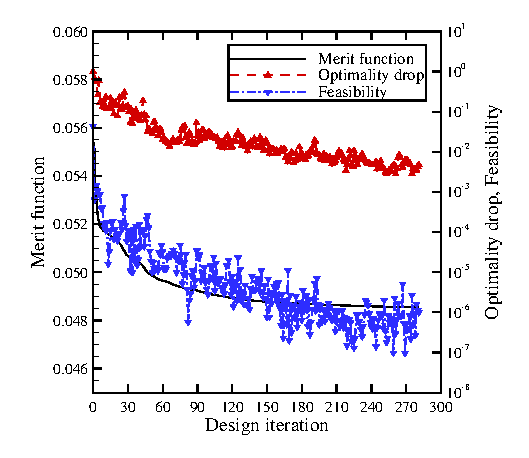
\includegraphics[trim={0.15cm 0cm 0.15cm 0cm},clip,width=3.175in]{Figures/With_Twist/A320neo/Optimize_A320_50deg.eps}}
    \caption{Convergence history for A320neo optimization with an upper sweep angle limit of 45.5\degree (\ref{fig:a320neo_converge_45.5_Deg}) and 50.2\degree (\ref{fig:a320neo_converge_50.0_Deg}).}
\label{fig:a320neo_planform_plots}
\end{figure}

% Similar to the NASA CRM's initial sweep optimization case, it was clear that this geometry has a very strong tendency to increase the wing sweep even further, as evidenced by the active wing sweep constraint very early on in the optimization. Performance also greatly increased when compared to a baseline trimmed flow solution for the same geometry, which was trimmed to an angle of attack that would satisfy the lift lift constraint of $C_L S=1.6686$, as seen in Table~\ref{tab:a320neo_results}. The drag coefficient $C_D S$ decreased by 101.1 drag counts with a small decrease in angle of attack. The $L/D$ also increased by over 5, from 27.89 to 33.58. This substantial improvement in efficiency motivated the decision to halt the optimization and start a new case with an increased sweep angle limit, as better performing optimum may be located at higher sweep angles, which was seen in the CRM optimization.

% As in the CRM optimization cases, the second A320neo case was run with a sweep angle limit expanded to 50.0\degree, which after converting to units of MAC and truncating, resulted in an upper sweep angle limit of 50.2\degree.
% This case was run for over 250 iterations. Continual decreases in the merit function, optimality, and feasibility were observed, as seen in Figure~\ref{fig:a320neo_converge_50.0_Deg}.

\begin{figure}[!tp]
\centering
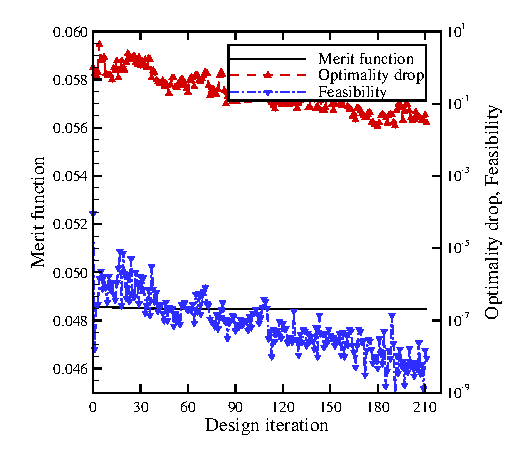
\includegraphics[width=4.5in]{Figures/With_Twist/A320neo/Optimize_A320_60deg.eps}
\caption{Convergence history for A320neo optimization with an upper sweep angle limit of 60.0\degree.}
\label{fig:a320neo_converge_60.0_Deg}
\end{figure}

% The merit function was seen to exhibit asymptotic behaviour after 150 design iterations, indicating that this case may have settled into a optimum. However, analysis of the optimization iteration history illustrated that just as in the CRM 50.0\degree\ case, the optimized geometry possesses a sweep angle close to the sweep angle limit of 50.2\degree, albeit not as close as the CRM 50.0\degree\ case. The sweep angle had increased to 46.90\degree, with corresponding improvements in $C_D S$ by 11.5 drag counts. The angle of attack increased by 0.056\degree, increasing from 2.103\degree\ to 2.159\degree—behaviour opposite to the CRM's trends. When converted to units of MAC, the margin between the optimized sweep angle and the upper sweep angle limit was 0.5385 reference units. This value is a much higher margin compared to the CRM 50.0\degree\ case, corresponding to approximately 20\% of the A320neo's 50.0\degree\ sweep limit of 2.750 reference units. The A320neo's sweep limit constraint was certainly inactive in this instance but it was decided that the sweep angle should be increased further to be thorough.

% The last A320neo case made use of the last optimized geometry from the 50.2\degree\ sweep limit case as its initial geometry. The upper sweep limit was expanded further to 60.0\degree, resulting in modifications to the upper sweep angle constraint as seen in Table~\ref{tab:a320neo-opt-60deg}.

\begin{table}[!tp]
\centering
\caption{Results summary for the optimization of the A320neo}
\label{tab:a320neo_results}
\begin{adjustbox}{center}
\begin{tabular}{lcccc}
\hline\hline
Design Variable & Trimmed Baseline & 37.7\degree\ Sweep Limit & 50.2\degree\ Sweep Limit & 60.0\degree\ Sweep Limit\\
\hline
$S$ (ref. units\textsuperscript{2}) & 3.340 & 3.339 & 3.339 & 3.338 \\
$C_L S$ & 1.669 & 1.669 & 1.669 & 1.669 \\
$C_M S$ & -0.736 & -1.399 & -2.280 & -2.254 \\
$C_D S$ (counts) & 598.2 & 497.0 & 485.5 & 484.7 \\
$L/D$ & 27.89 & 33.58 & 34.37 & 34.42 \\
Angle of Attack & 2.303\degree\ & 2.103\degree\ & 2.159\degree\ & 2.026\degree\ \\
\makecell[l]{Post-Optimization\\Leading Edge Sweep Angle} & 27.9\degree\ & 37.68\degree\ & 46.90\degree\ & 46.74\degree\ \\
\hline\hline
\end{tabular}
\end{adjustbox}
\end{table}

% This case was run for over 200 iterations, and observed no significant changes to the merit function. The optimality dropped one order of magnitude, whereas the feasibility decreased by three orders of magnitude to approximately $10^{-9}$, as seen in Figure~\ref{fig:crm_converge_60.0_Deg}. 

The result from the 60.0\degree\ sweep limit case indicates that it is simply a further convergence on the result from the 50.2\degree\ case. The geometry did not change significantly compared to the 50.2\degree\ sweep limit case. Just as in the CRM 60.0\degree\ case, the sweep limit decreased from the A320neo 50.2\degree\ case's most optimal point, dropping 0.16\degree\ from 46.90\degree\ to 46.64\degree, as seen in Table~\ref{tab:a320neo_results}. Performance compared to the trimmed baseline shows that the $C_D S$ decreased by 113.4 drag counts to 484.7, the $L/D$ increased by 6.52 to 34.42, and the angle of attack decreased by 0.277\degree\ to 2.026\degree. Plots of the upper surface pressure contours for the trimmed baseline flow solution and the 60.0\degree\ sweep limit optimized planform are shown in Figure~\ref{fig:a320neo_planform_plots}. Plots of the section geometry and pressure distribution at various spanwise sections for the trimmed baseline flow solution and the 60.0\degree\ sweep limit optimized planform are shown in Figure~\ref{fig:a320neo_section_plots}.

Just as in the CRM case, the A320neo's original geometry exhibits a shock along the entire span of the wing, as seen in Figures~\ref{fig:a320neo_baseline_planform} and~\ref{fig:a320neo_section_plots}. The optimized geometry resulting from the 60.0\degree\ sweep limit is able to completely remove this shock. Furthermore, with the exception of the root and wingtip, the optimizer is able to produce a smooth pressure recovery over the wing, as seen in Figures~\ref{fig:a320neo_section_20.6_perc}-\ref{fig:a320neo_section_79.4_perc}.

\begin{figure}[!tp]
    \centering
    \subfloat[\label{fig:a320neo_baseline_planform}]{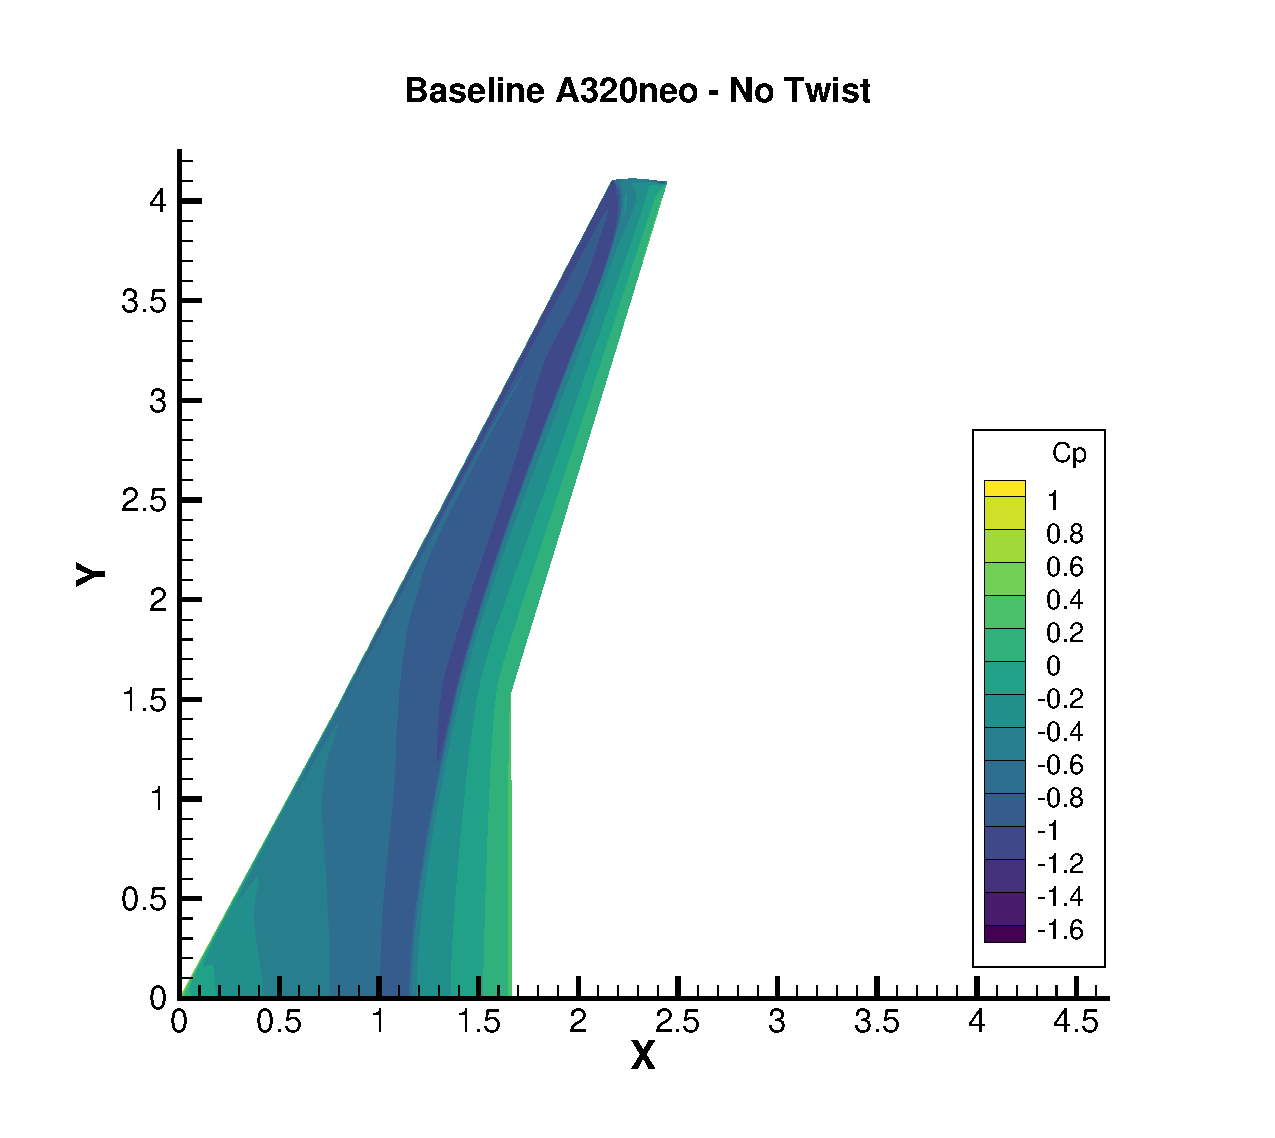
\includegraphics[trim={0.25cm 0.25cm 0.25cm 0.25cm},clip,width=3.175in]{Figures/With_Twist/A320neo/A320neo_Baseline-Contour-Upper.eps}}
    \hspace{0.25cm}
    \subfloat[\label{fig:a320neo_60_deg_planform}]{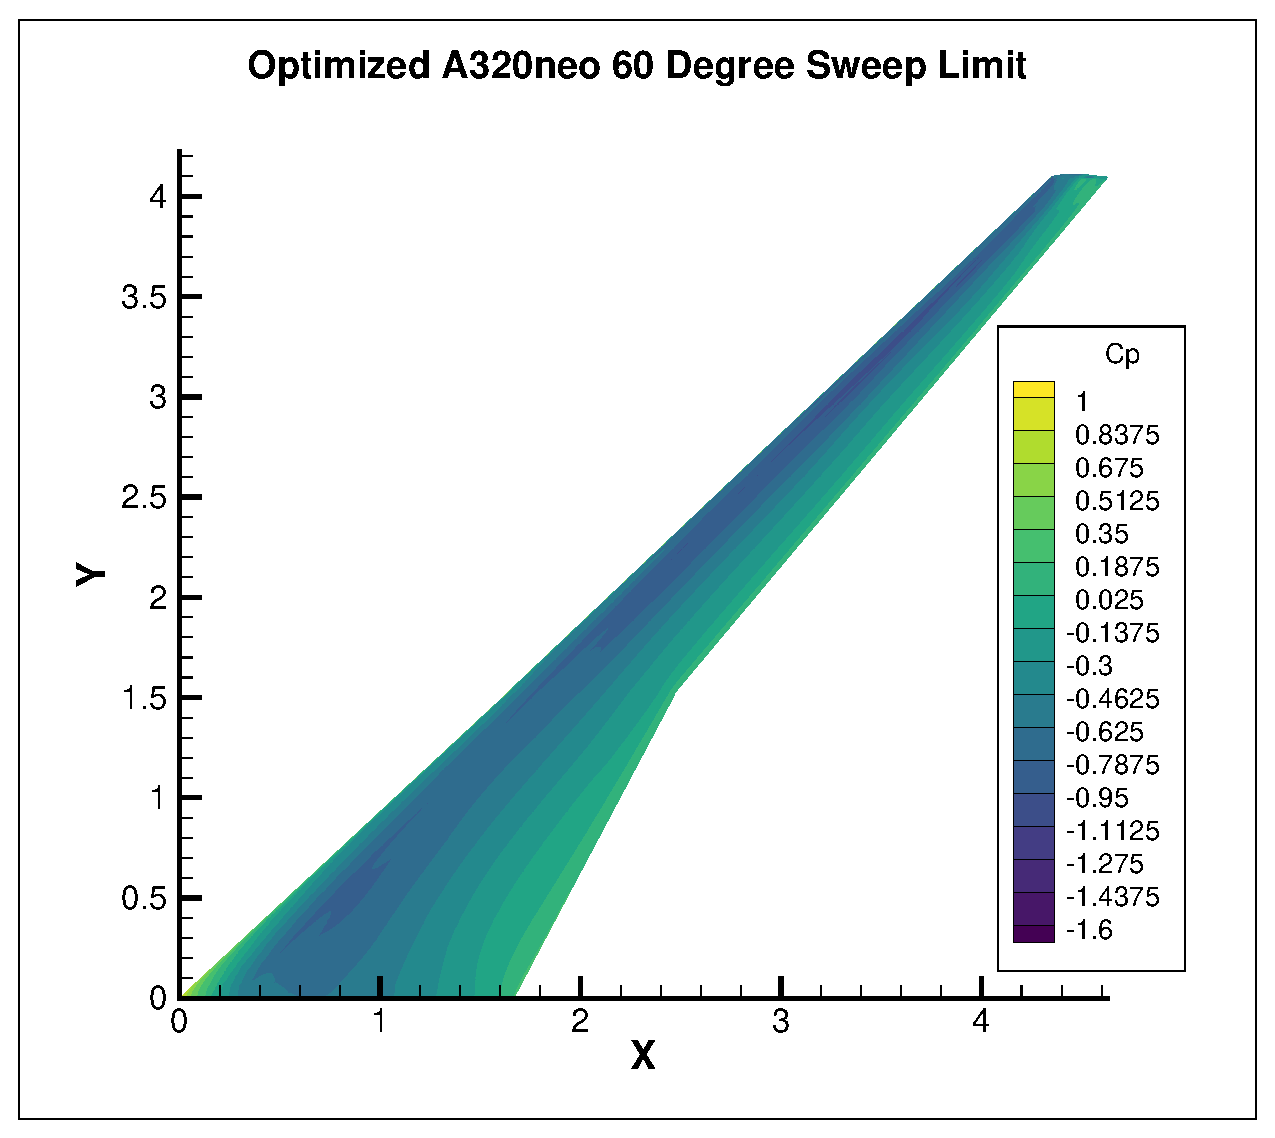
\includegraphics[trim={0.25cm 0.25cm 0.25cm 0.25cm},clip,width=3.175in]{Figures/With_Twist/A320neo/A320neo_varsweep_60deg-Contour-Upper.eps}}
    \caption{A320neo upper surface pressure contours for the trimmed angle of attack baseline planform (\ref{fig:a320neo_baseline_planform}) and 60.0\degree\ sweep angle limit optimized planform (\ref{fig:a320neo_60_deg_planform}).}
\label{fig:a320neo_planform_plots}
\end{figure}

\begin{figure}[!tp]
    \centering
    \subfloat[\label{fig:a320neo_section_1_perc}]{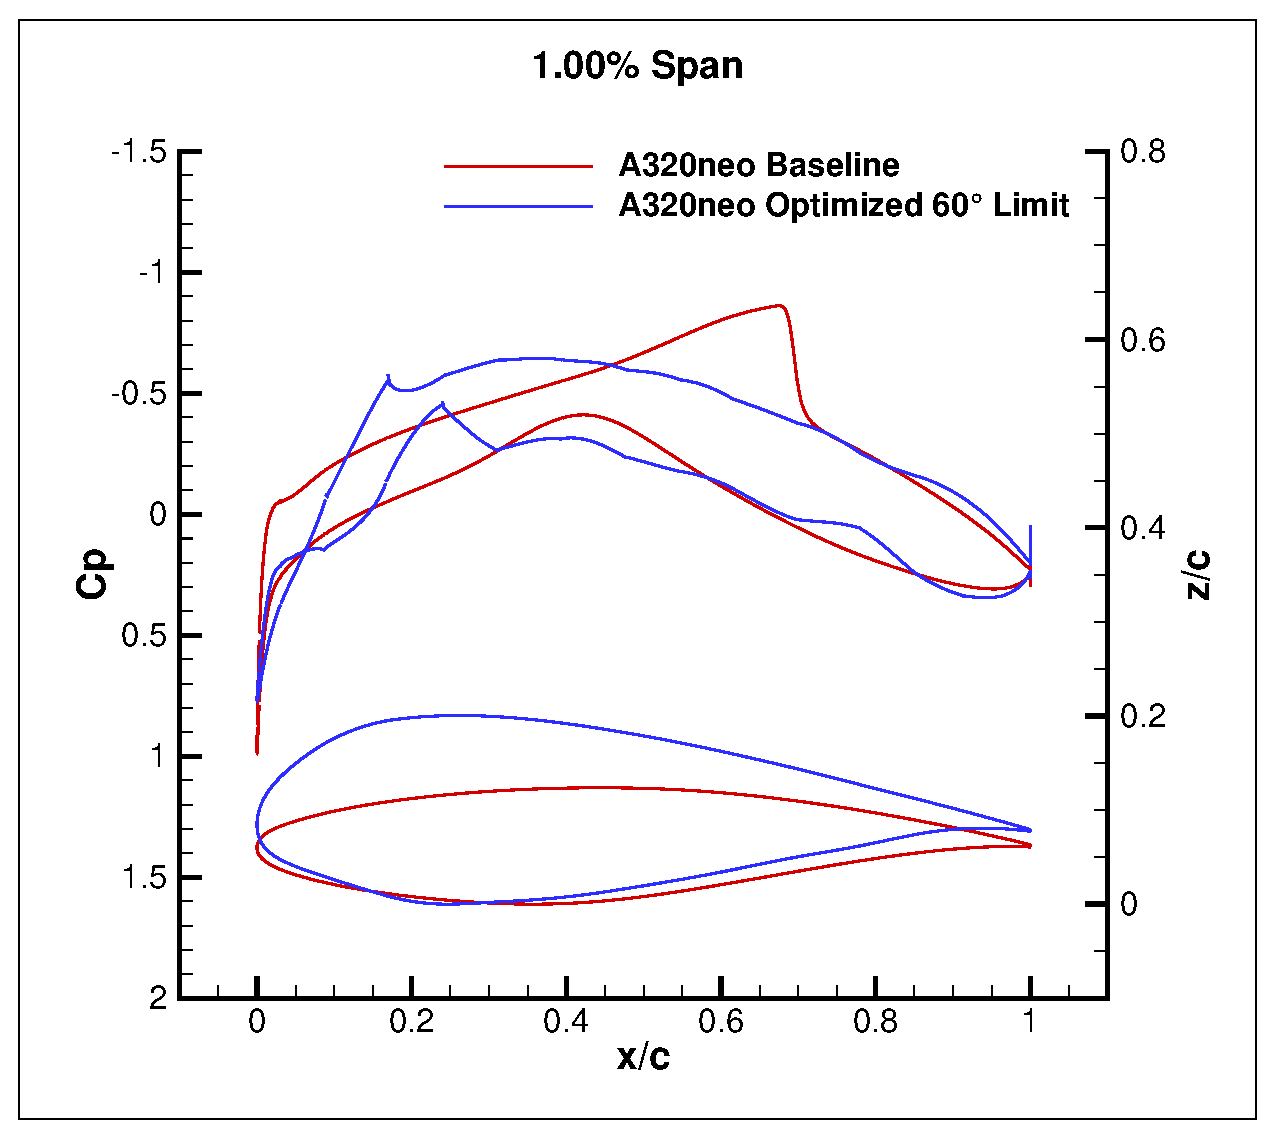
\includegraphics[trim={0.25cm 0.25cm 0.25cm 0.25cm},clip,width=3in]{Figures/With_Twist/A320neo/A320neo_1.00percent_Span.eps}}
    \hspace{0.25cm}
    \subfloat[\label{fig:a320neo_section_20.6_perc}]{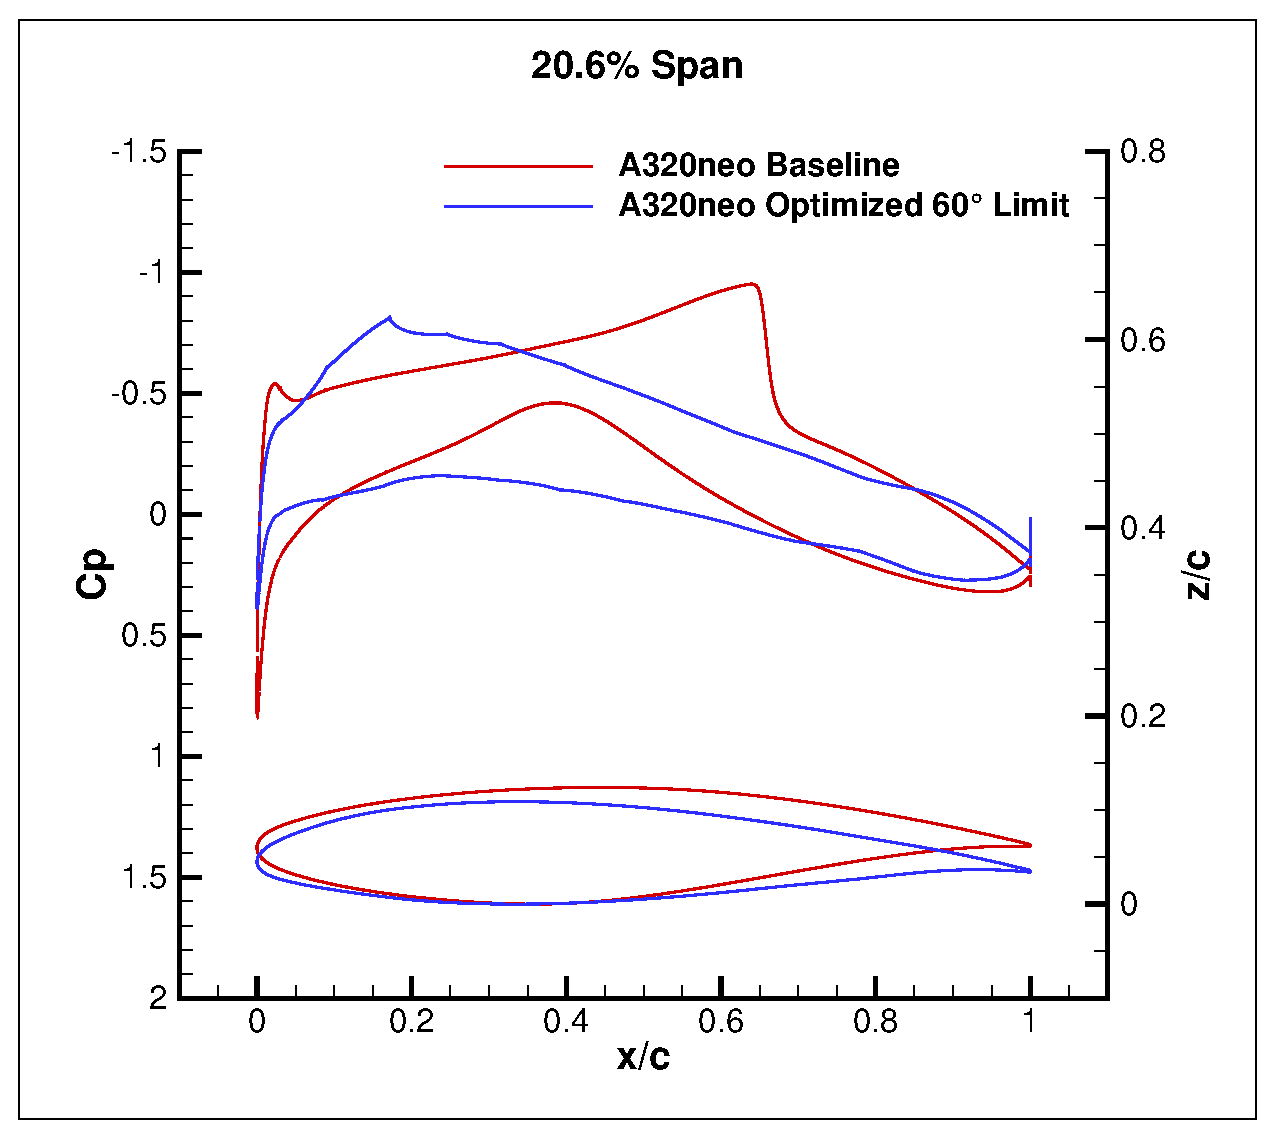
\includegraphics[trim={0.25cm 0.25cm 0.25cm 0.25cm},clip,width=3in]{Figures/With_Twist/A320neo/A320neo_20.6percent_Span.eps}}\\
    \subfloat[\label{fig:a320neo_section_40.2_perc}]{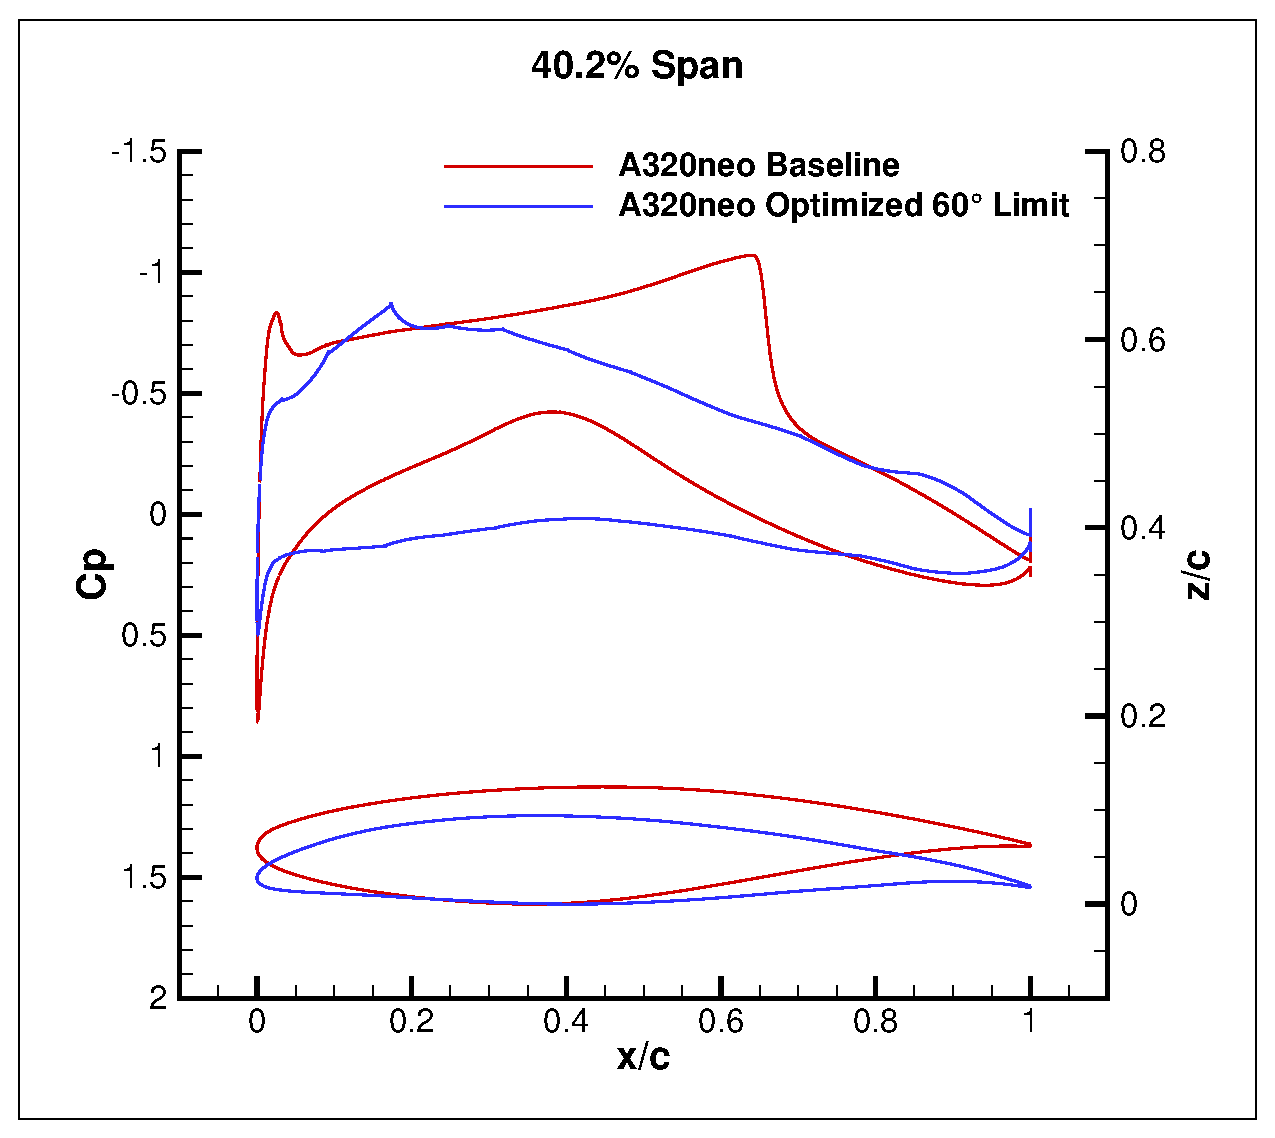
\includegraphics[trim={0.25cm 0.25cm 0.25cm 0.25cm},clip,width=3in]{Figures/With_Twist/A320neo/A320neo_40.2percent_Span.eps}}
    \hspace{0.25cm}
    \subfloat[\label{fig:a320neo_section_59.8_perc}]{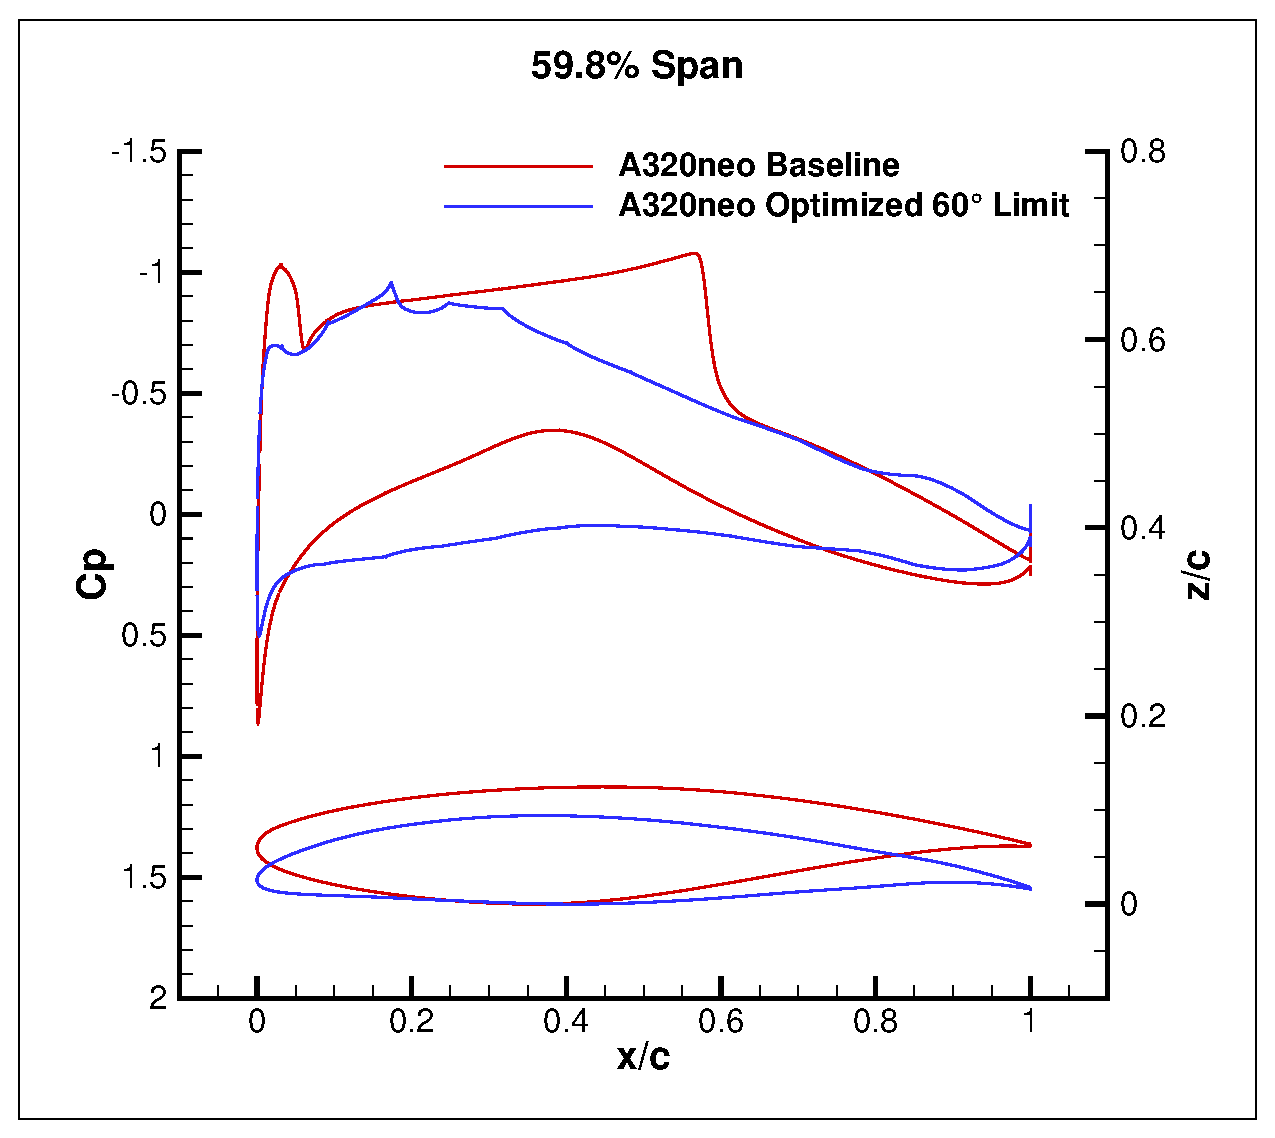
\includegraphics[trim={0.25cm 0.25cm 0.25cm 0.25cm},clip,width=3in]{Figures/With_Twist/A320neo/A320neo_59.8percent_Span.eps}}\\
    \subfloat[\label{fig:a320neo_section_79.4_perc}]{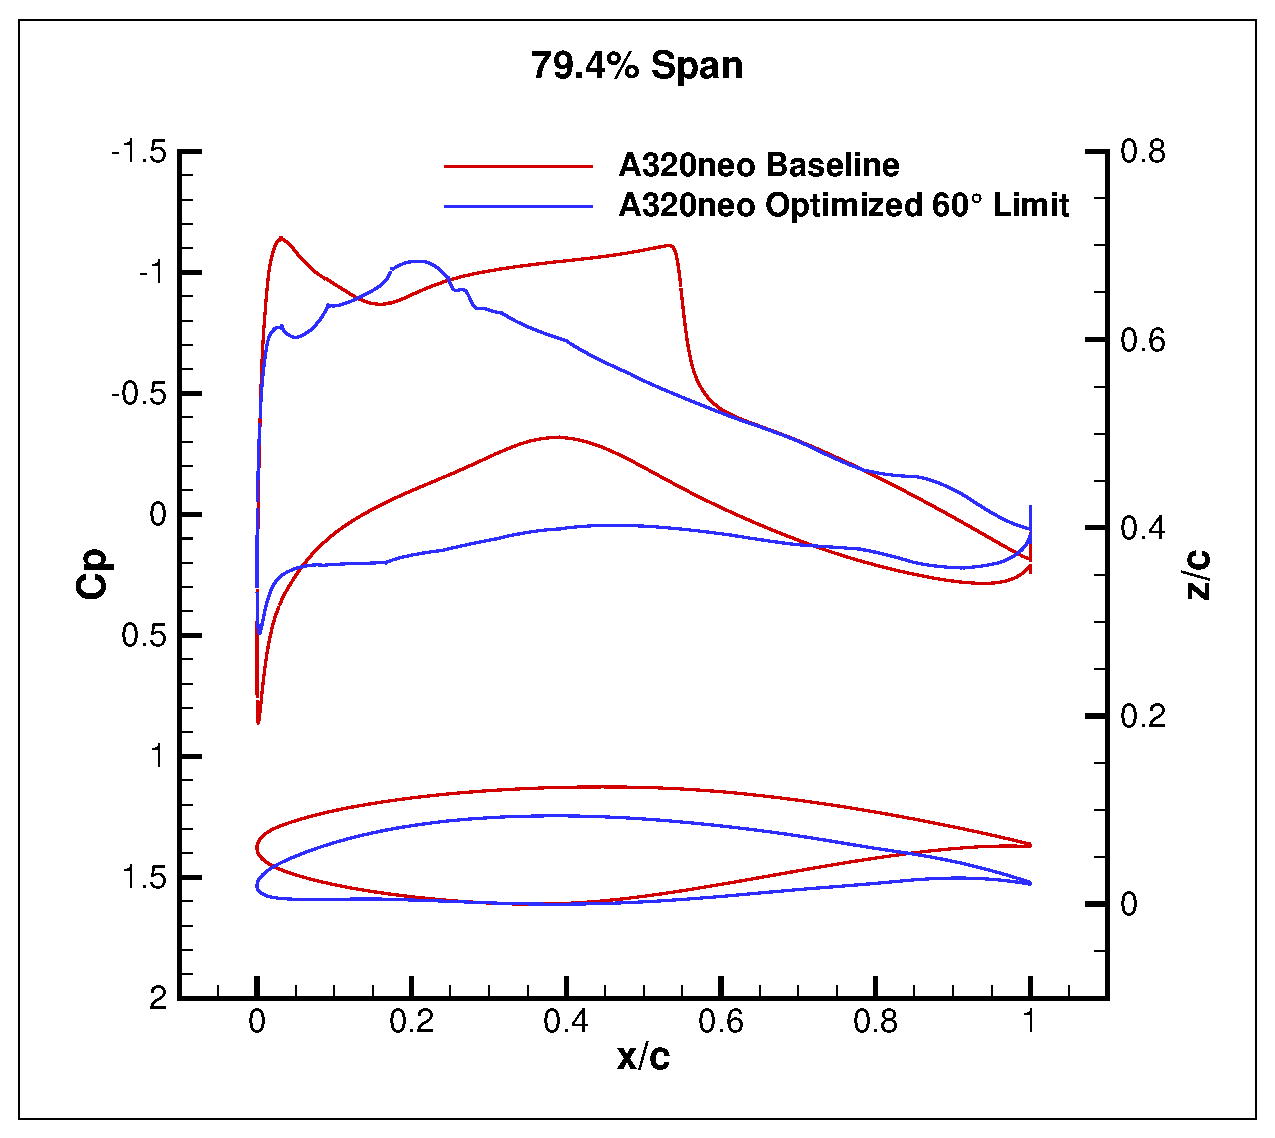
\includegraphics[trim={0.25cm 0.25cm 0.25cm 0.25cm},clip,width=3in]{Figures/With_Twist/A320neo/A320neo_79.4percent_Span.eps}}
    \hspace{0.25cm}
    \subfloat[\label{fig:a320neo_section_99.0_perc}]{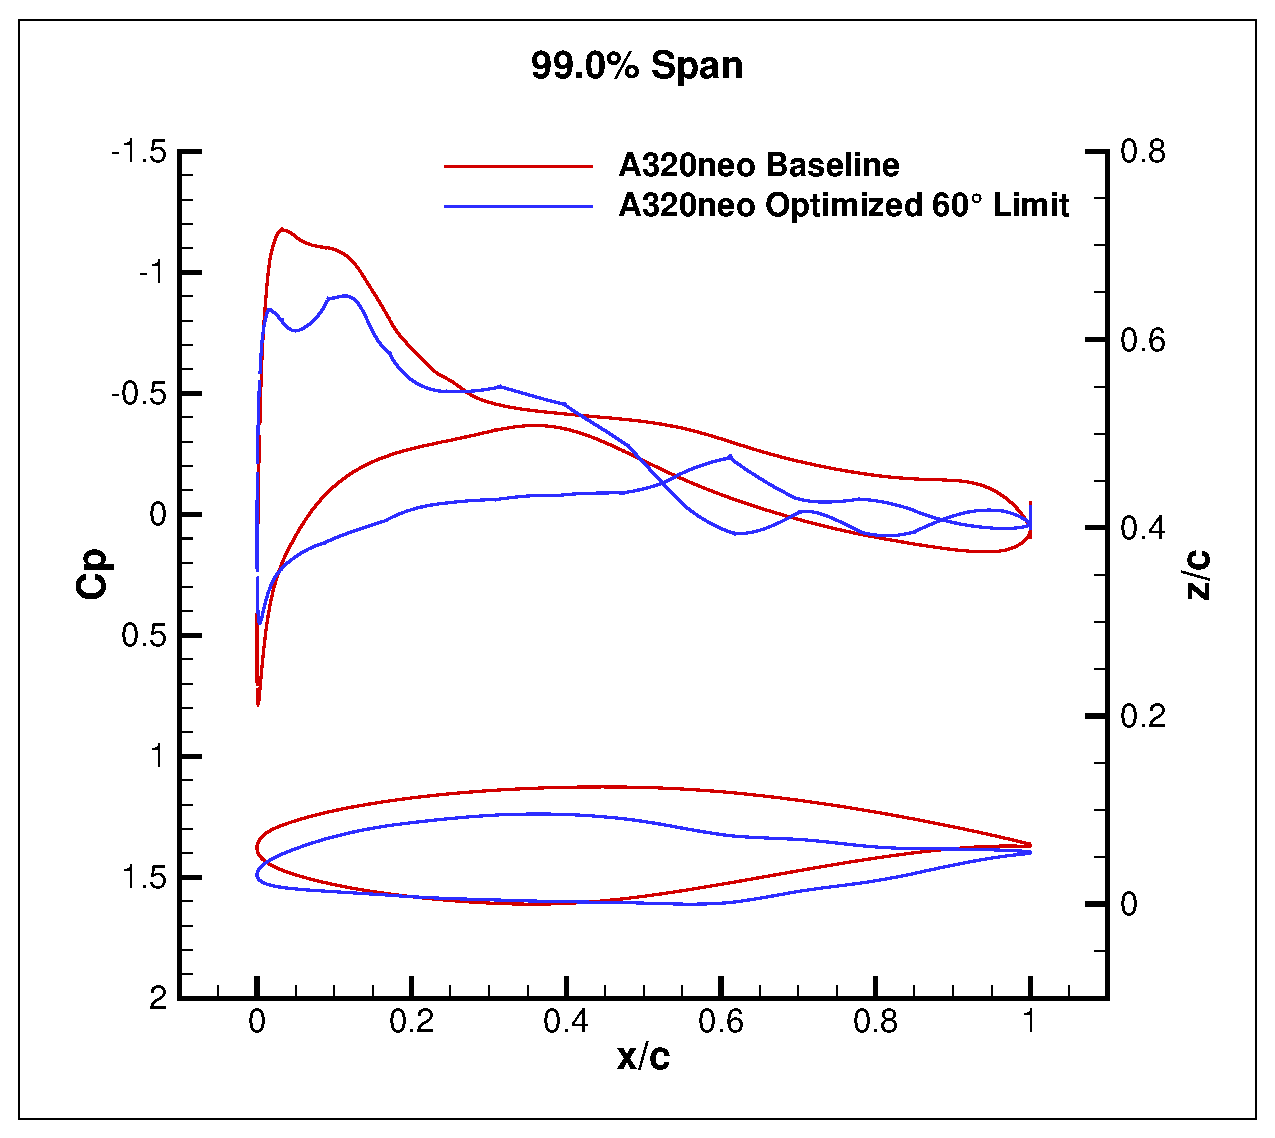
\includegraphics[trim={0.25cm 0.25cm 0.25cm 0.25cm},clip,width=3in]{Figures/With_Twist/A320neo/A320neo_99.0percent_Span.eps}}
    \caption{Section geometry and pressure distribution plots of the trimmed angle of attack A320neo baseline planform and 60.0\degree\ sweep angle limit optimized planform at 1.00\% (\ref{fig:a320neo_section_1_perc}), 20.6\% (\ref{fig:a320neo_section_20.6_perc}), 40.2\% (\ref{fig:a320neo_section_40.2_perc}), 59.8\% (\ref{fig:a320neo_section_59.8_perc}), 79.4\%(\ref{fig:a320neo_section_79.4_perc}), and 99.0\% (\ref{fig:a320neo_section_99.0_perc}) span.}
\label{fig:a320neo_section_plots}
\end{figure}
\FloatBarrier

The section shape of the optimized wing differs greatly from the baseline geometry, although in slightly different ways compared to the CRM optimized wing. The thickness is greatly increased at the root and is continuously reduced along the remainder of the wingspan compared to the initial geometry. Since this case included a minimum volume constraint, this behaviour is expected and aligns with the results of other studies~\cite{ledoux_study_2015, kenway_multipoint_2015, telidetzki_application_2014, lyu_rans-based_2014, lyu_aerodynamic_2015, osusky_drag_2015, shi-dong_approximate_2018, yu_influence_2018, koo_investigation_2018}. The camber is reduced at almost all spanwise points with the exception of the wingtip, where strange behaviour occurs. As seen in Figure~\ref{fig:a320neo_section_99.0_perc}, a complex section shape is produced. This feature is similar to the wingtip section shape produced in the CRM 60.0\degree\ twist-inclusive optimization case, and it is unclear why it occurred in this case as well.
% However, the trailing half of the wing appears to be at a greater twist relative to the CRM section at 79.4\% span in Figure~\ref{fig:crm_section_79.4_perc}, which differs compared to the CRM case. The overall twist at 99.0\% span appears to be a marginal increase compared to the original geometry, but it is unclear why this result has occurred. 
Just as in the CRM case, the spanwise sections used for measurement in this study differ from those specified in ADODG Case 4 and reported in other studies~\cite{martins_aerodynamic_2022, koo_investigation_2018, shi-dong_adjoint-based_2017, lyu_aerodynamic_2015, kenway_multipoint_2015}, such that the root and wingtip sections measured in this study are not the same as those used in ADODG Case 4. Again, it is possible that analysis of the sections using the spanwise points dictated by ADODG Case 4 may show that such artifacts do not occur when measuring at 94.4\% span as specified by ADODG Case 4, compared to measurements at 99.0\% span as used in this study.

%%%%%%%%%%%%%%%%%% TALK ABOUT WEIRD TWIST BEHAVIOUR HERE %%%%%%%%%%%%%%%%%%
The wing artifact occurring at 99.0\% span seen in the NASA CRM geometry also occurs on the A320neo, as seen in Figure~\ref{fig:a320neo_section_99.0_perc}. Oscillations in wing twist occurred as well, as seen in Figure~\ref{fig:a320neo_artifact}. These oscillations are lower in amplitude compared to those seen on the NASA CRM 60.0\degree\ case with wing twist. Just as in the NASA CRM study, a secondary optimization was conducted on the A320neo with an otherwise identical methodology to that in section~\ref{ssec-prob-formulate}, with the exception of wing twist as a design variable and the selection of sweep limits, which are described in the following section.

\begin{figure}[!tp]
    \centering
    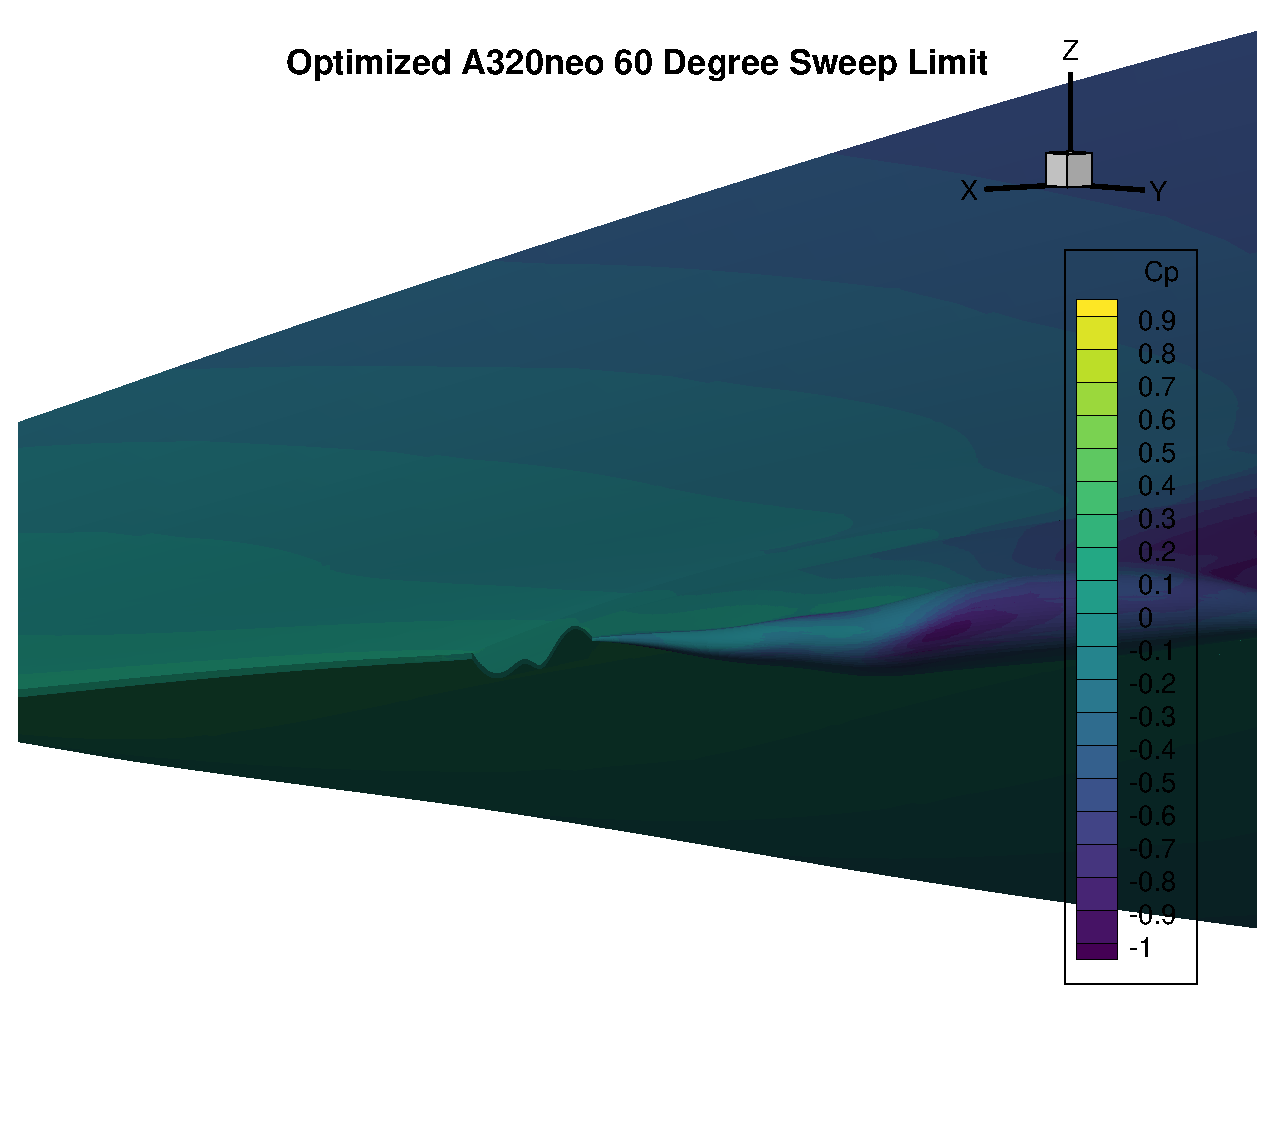
\includegraphics[width=4.5in]{Figures/With_Twist/A320neo/Optimize_A320_60deg_Twist_Artifact_01.eps}
    \caption{Trailing edge geometry artifacts observed in the A320neo 60.0\degree\ sweep angle limit optimized planform.}
\label{fig:a320neo_artifact}
\end{figure}
\FloatBarrier

%%%%%%%%%%%%%%%%%% INTRODUCE NEW CASE WITHOUT TWIST %%%%%%%%%%%%%%%%%%

\subsection{A320neo Optimization without Wing Twist}
\label{ssec:a320neo-opt-notwist}
Similar to the twist-deactivated study performed on the CRM wing, a second study was performed on the A320neo without wing twist as a design variable. In these cases, the local wing twist was required to be equal to 0\degree\ every where on the wing. Based on the results obtained in the initial A320neo ASO cases, the sweep angle limit was expanded to 60.0\degree.

An additional study was conducted on the A320neo without wing twist at its original sweep angle of 27.9\degree\ as well. Just as in the CRM twist-deactivated cases, this optimization result served to provide context for the 60.0\degree\ sweep limit result without wing twist, as ASO on section shape and angle of attack at an aircraft's original sweep angle is the most accessible way to performance on a conventional aircraft, and is also the approach that is conducted most often~\cite{lyu_rans-based_2014, lyu_aerodynamic_2015, osusky_drag_2015, streuber_investigation_2017, koo_investigation_2018}. Wing twist is typically included as well, but the geometry artifacts obtained when twist was included as a design variable motivated its exclusion from a fixed sweep angle ASO at the A320neo's original sweep angle.

The fixed sweep angle A320neo ASO at the original sweep angle of 27.9\degree\ exhibited smooth optimization progress, with qualitative analysis of the merit function, optimality, and feasibility demonstrating that convergence was obtained after 326 design iterations, as seen in Figure~\ref{fig:a320neo_notwist_converge_baseline}. The drag coefficient $C_D S$ decreased by 98.5 drag counts relative to the trimmed baseline wing, the $L/D$ increased by 5.5, and the angle of attack decrease by over 0.5\degree, as seen in Table~\ref{tab:a320neo_notwist_results}.

The A320neo ASO without twist at a sweep angle limit of 60.0\degree\ demonstrated similarly smooth optimization progress compared to the previous twist-deactivated case. Analysis of the merit function, optimality, and feasibility illustrated that convergence was achieved after 388 design iterations, as seen in Figure~\ref{fig:a320neo_notwist_converge_60.0_Deg}. The drag coefficient decreased by 112.6 drag counts relative to the trimmed baseline wing, with a less than 0.1\degree\ decrease in the angle of attack. The moment coefficient decreased considerably by over 1.5, lowering from -0.736 to -2.268. The $L/D$ increased by almost 6.5 counts, rising from 27.89 to 34.37. While this is a substantial improvement over the trimmed baseline wing, it is only a 2.83\% improvement over the A320neo optimized at the original sweep angle of 27.9\degree, despite an increase in the wing sweep of almost 19\degree.

%%%%%% A320neo NO TWIST CONVERGENCE PLOTS %%%%%%
\begin{figure}[!tp]
\centering
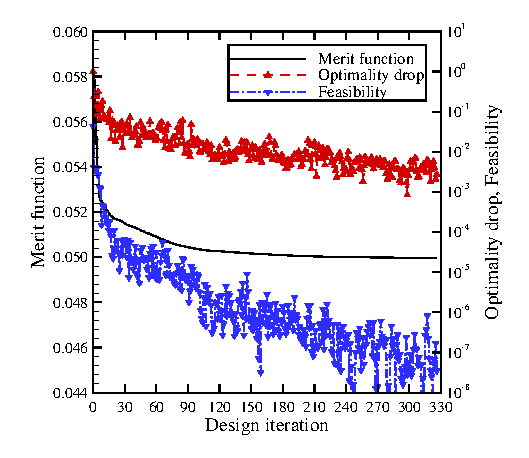
\includegraphics[width=4.5in]{Figures/No_Twist/A320neo/Optimize_A320_Fixed_Orig_No_Twist.eps}
\caption{Convergence history for A320neo optimization without wing twist with a sweep angle limit at the original sweep angle of 27.9\degree.}
\label{fig:a320neo_notwist_converge_baseline}
\end{figure}

\begin{figure}[!tp]
\centering
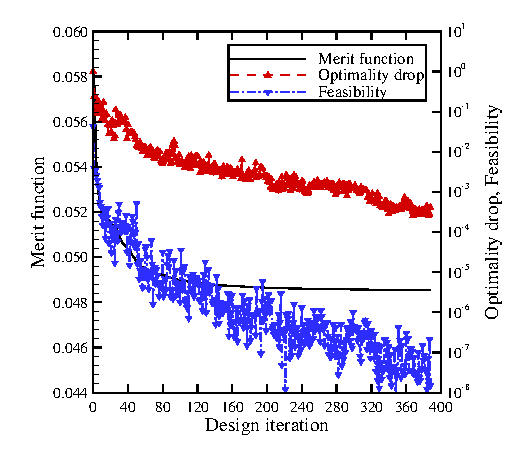
\includegraphics[width=4.5in]{Figures/No_Twist/A320neo/Optimize_A320_No_Twist_60deg.eps}
\caption{Convergence history for A320neo optimization without wing twist with an upper sweep angle limit of 60.0\degree.}
\label{fig:a320neo_notwist_converge_60.0_Deg}
\end{figure}

%%%%%% A320neo NO TWIST RESULTS TABLE %%%%%%
\begin{table}[!tp]
\centering
\caption{Results summary for the optimization of the A320neo without wing twist}
\label{tab:a320neo_notwist_results}
\begin{adjustbox}{center}
\begin{tabular}{lcccc}
\hline\hline
Design Variable & Trimmed Baseline & Original (27.9\degree)\ Sweep Limit & 60.0\degree\ Sweep Limit\\
\hline
$S$ (ref. units\textsuperscript{2}) & 3.340 & 3.340 & 3.340 \\
$C_L S$ & 1.669 & 1.667 & 1.667 \\
$C_M S$ & -0.736 & -0.752 & -2.268 \\
$C_D S$ (counts) & 598.2 & 499.7 & 485.6 \\
$L/D$ & 27.89 & 33.39 & 34.37 \\
Angle of Attack & 2.303\degree\ & 1.655\degree\ & 2.238\degree\ \\
\makecell[l]{Post-Optimization\\Leading Edge Sweep Angle} & 27.9\degree\ & 27.89\degree\ & 46.67\degree\ \\
\hline\hline
\end{tabular}
\end{adjustbox}
\end{table}

Plots of the pressure contours on the upper surface of the A320neo ASOs without wing twist are shown in Figure~\ref{fig:a320neo_notwist_planform_plots}. Plots of the section shape and pressure distribution at numerous spanwise sections are presented in Figure~\ref{fig:a320neo_notwist_section_plots}, which include the trimmed angle of attack baseline, the fixed-sweep ASO at the original sweep angle of 27.9\degree\ and the 60.0\degree\ sweep limit ASO.

%%%%%% A320neo NO TWIST PLANFORM PLOTS %%%%%%
\begin{figure}[!tp]
    \centering
    \subfloat[\label{fig:a320neo_notwist_opt_baseline_planform}]{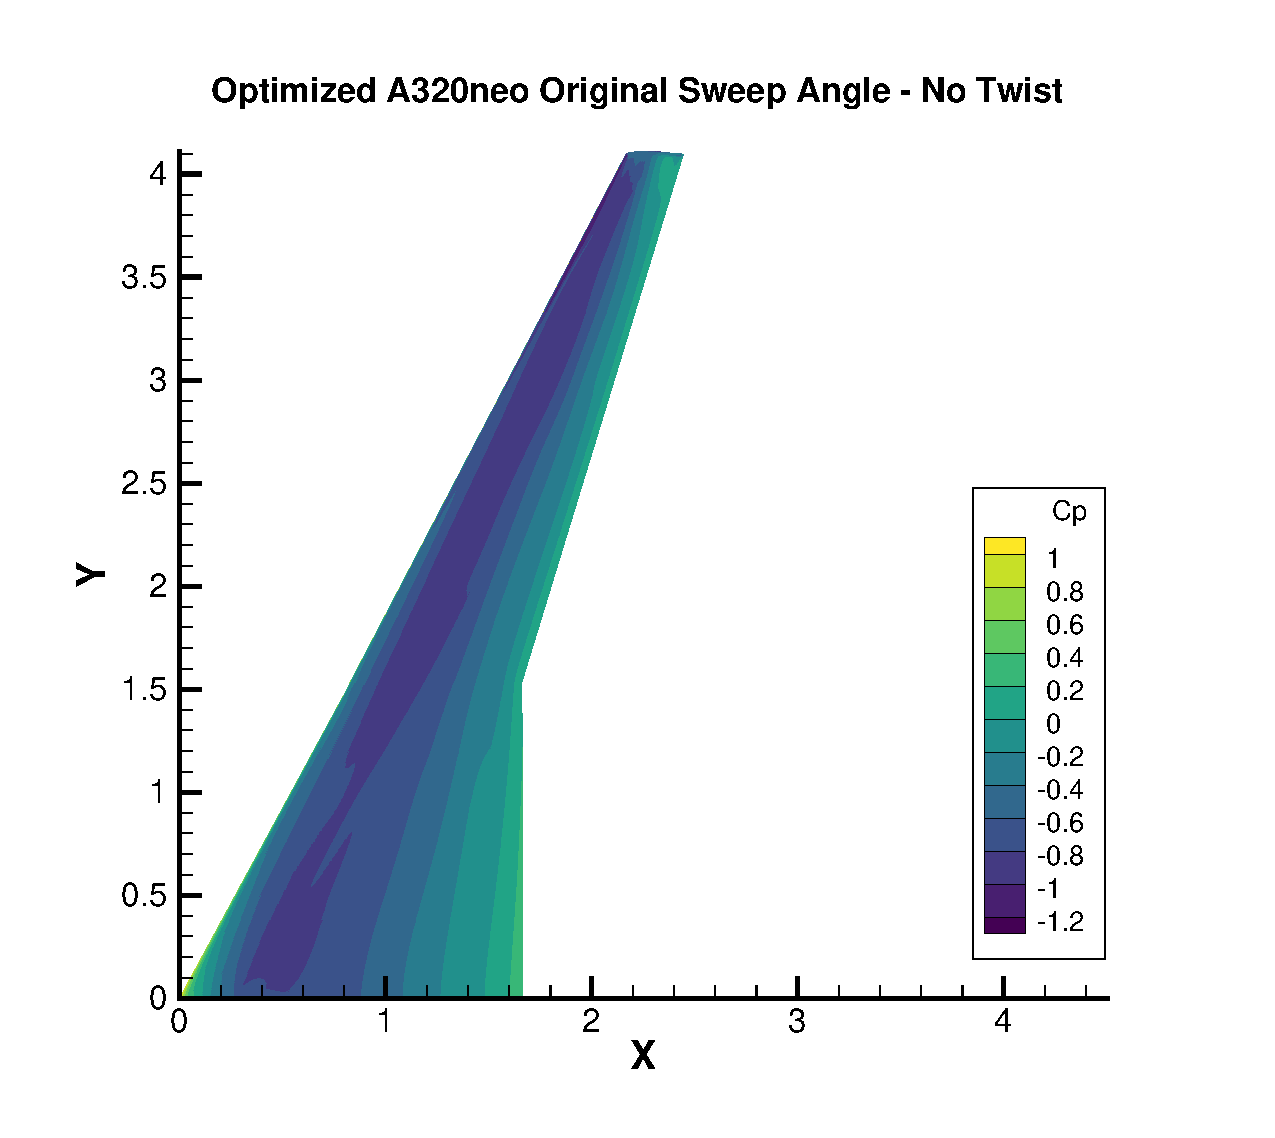
\includegraphics[trim={0.25cm 0.25cm 0.25cm 0.25cm},clip,width=3.175in]{Figures/No_Twist/A320neo/A320_Fixed_Orig_No_Twist-Contour-Upper.eps}}
    \hspace{0.25cm}
    \subfloat[\label{fig:a320neo_notwist_60_deg_planform}]{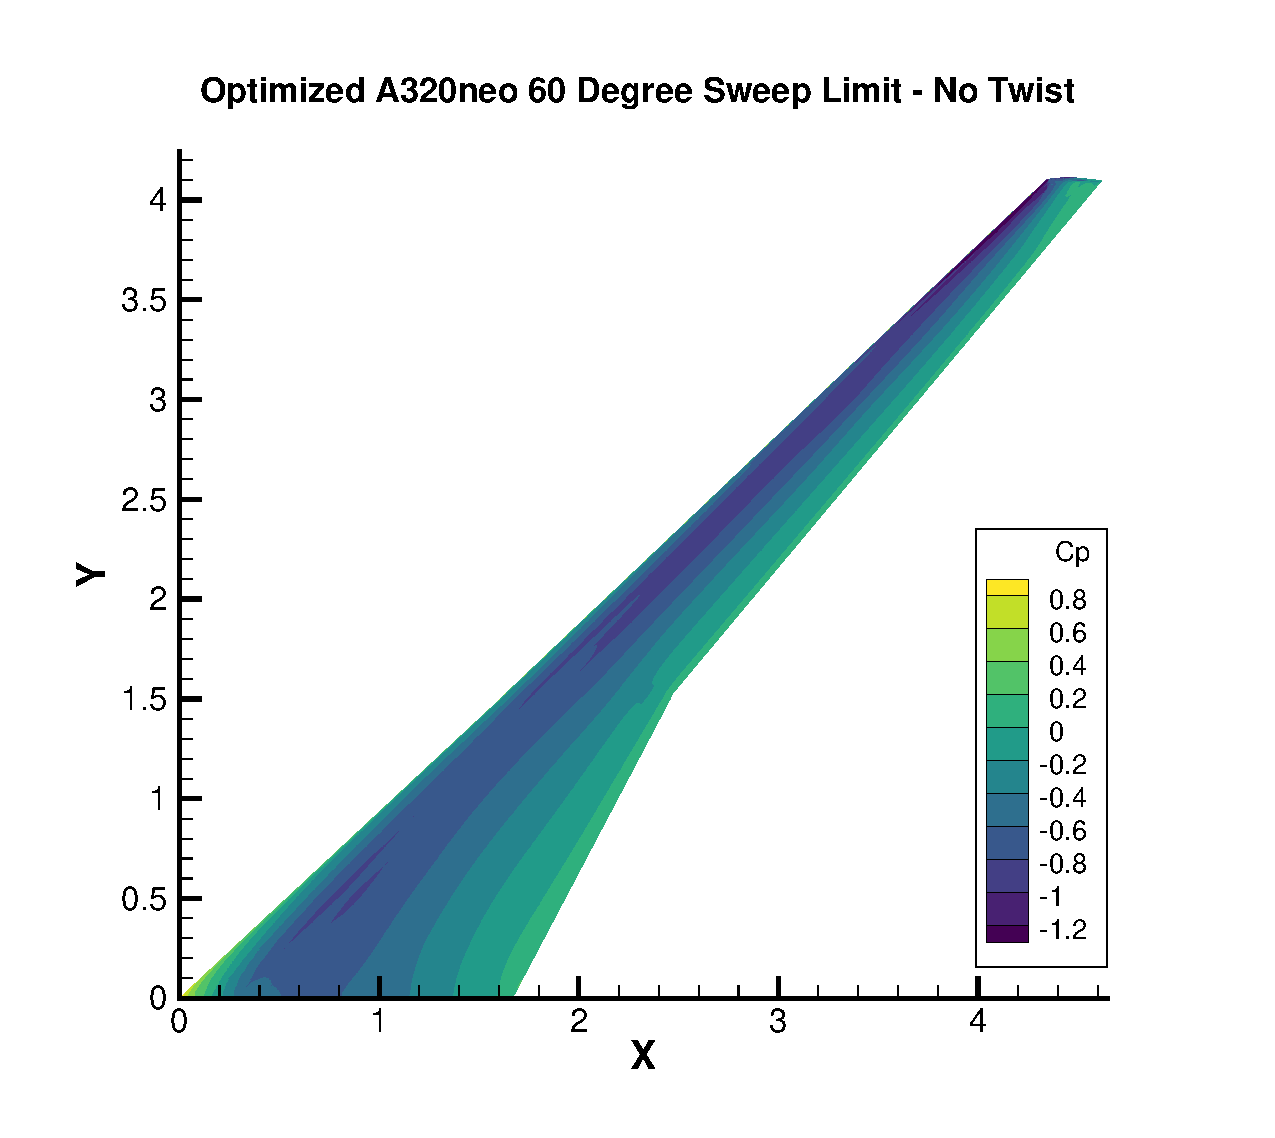
\includegraphics[trim={0.25cm 0.25cm 0.25cm 0.25cm},clip,width=3.175in]{Figures/No_Twist/A320neo/A320neo_varsweep_NoTwist_60deg-Contour-Upper.eps}}
    \caption{A320neo upper surface pressure contours for the original sweep angle limit optimized planform (\ref{fig:a320neo_notwist_opt_baseline_planform}) and 60.0\degree\ sweep angle limit optimized planform (\ref{fig:a320neo_notwist_60_deg_planform}) without wing twist in optimization.}
\label{fig:a320neo_notwist_planform_plots}
\end{figure}
\FloatBarrier

%%%%%% A320neo NO TWIST SECTION PLOTS %%%%%%
\begin{figure}[!tp]
    \centering
    \subfloat[\label{fig:a320neo_notwist_section_1_perc}]{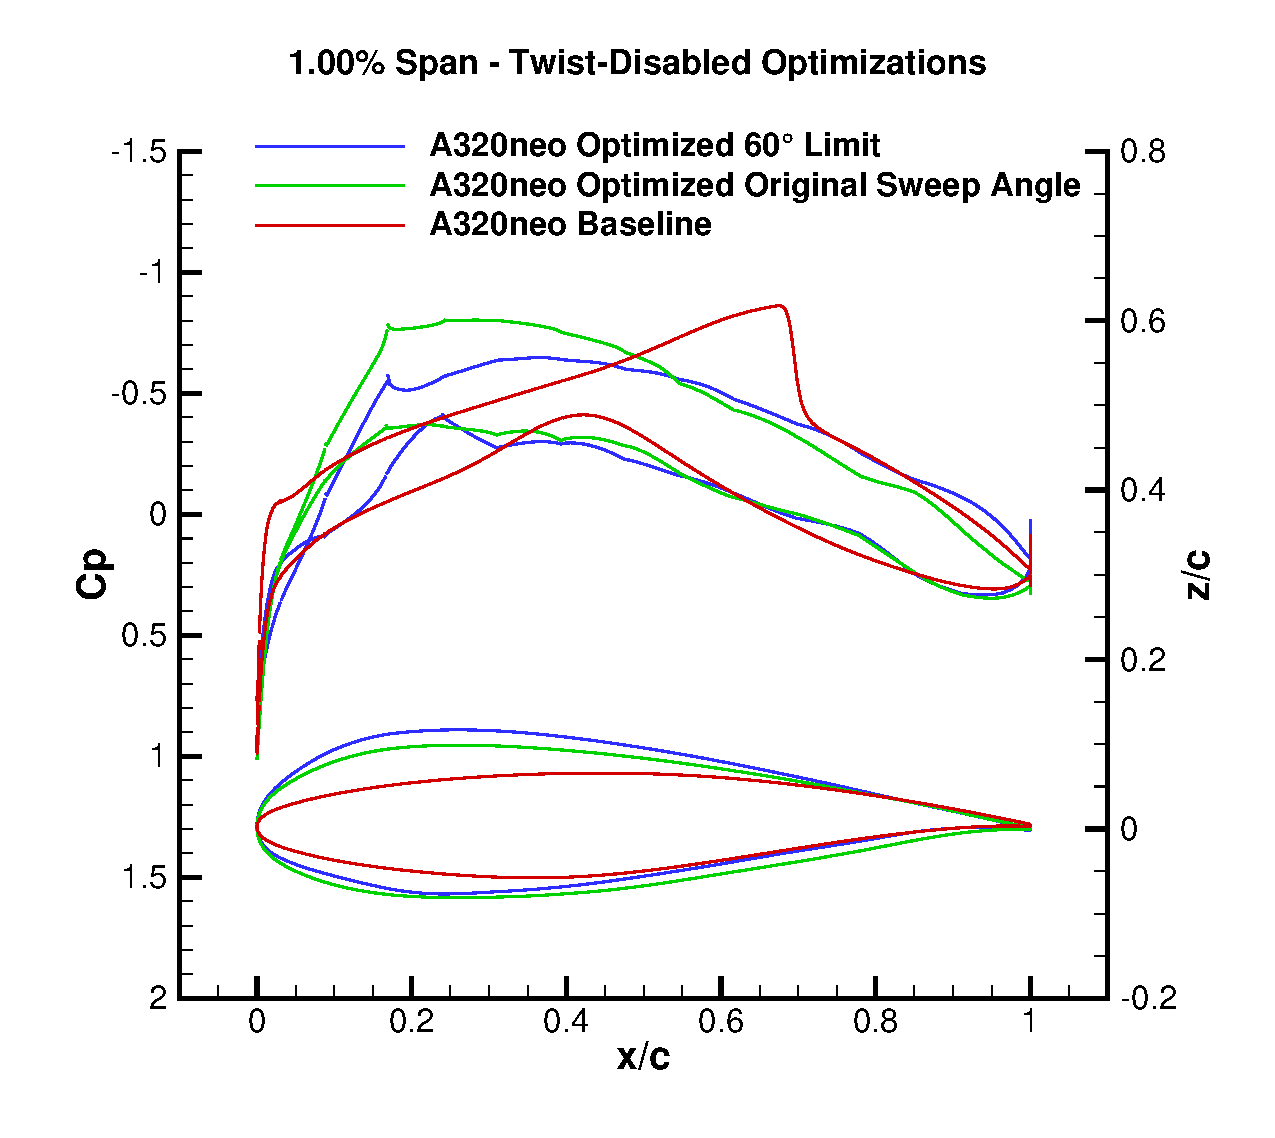
\includegraphics[trim={0.25cm 0.25cm 0.25cm 0.25cm},clip,width=3in]{Figures/No_Twist/A320neo/A320neo_Optimize_NoTwist-1.00percent_Span.eps}}
    \hspace{0.25cm}
    \subfloat[\label{fig:a320neo_notwist_section_20.6_perc}]{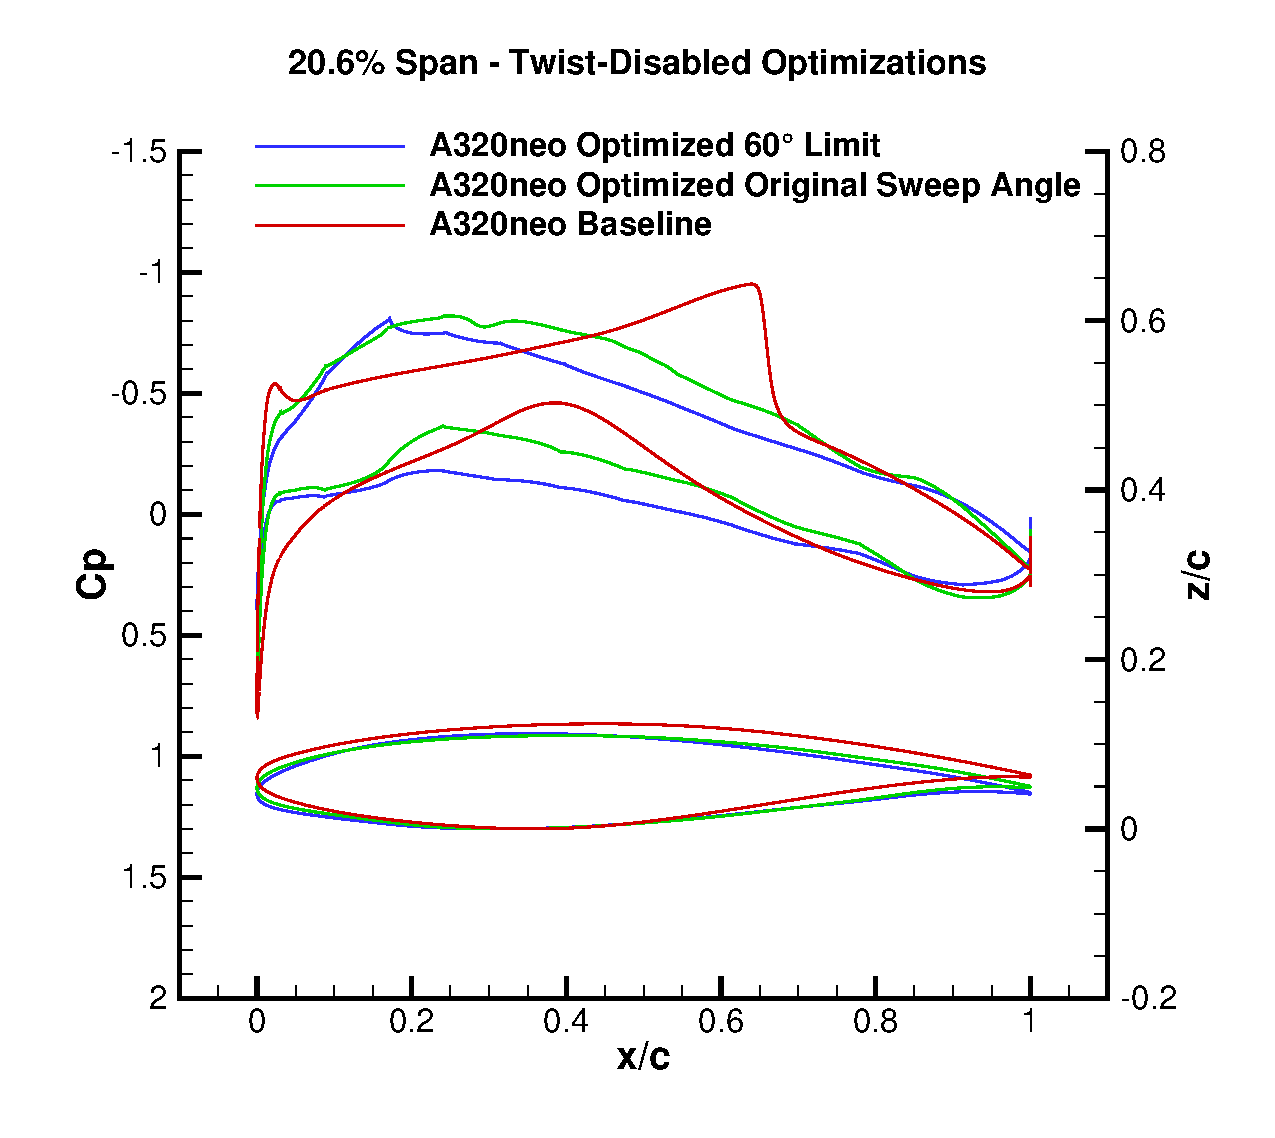
\includegraphics[trim={0.25cm 0.25cm 0.25cm 0.25cm},clip,width=3in]{Figures/No_Twist/A320neo/A320neo_Optimize_NoTwist-20.6percent_Span.eps}}\\
    \subfloat[\label{fig:a320neo_notwist_section_40.2_perc}]{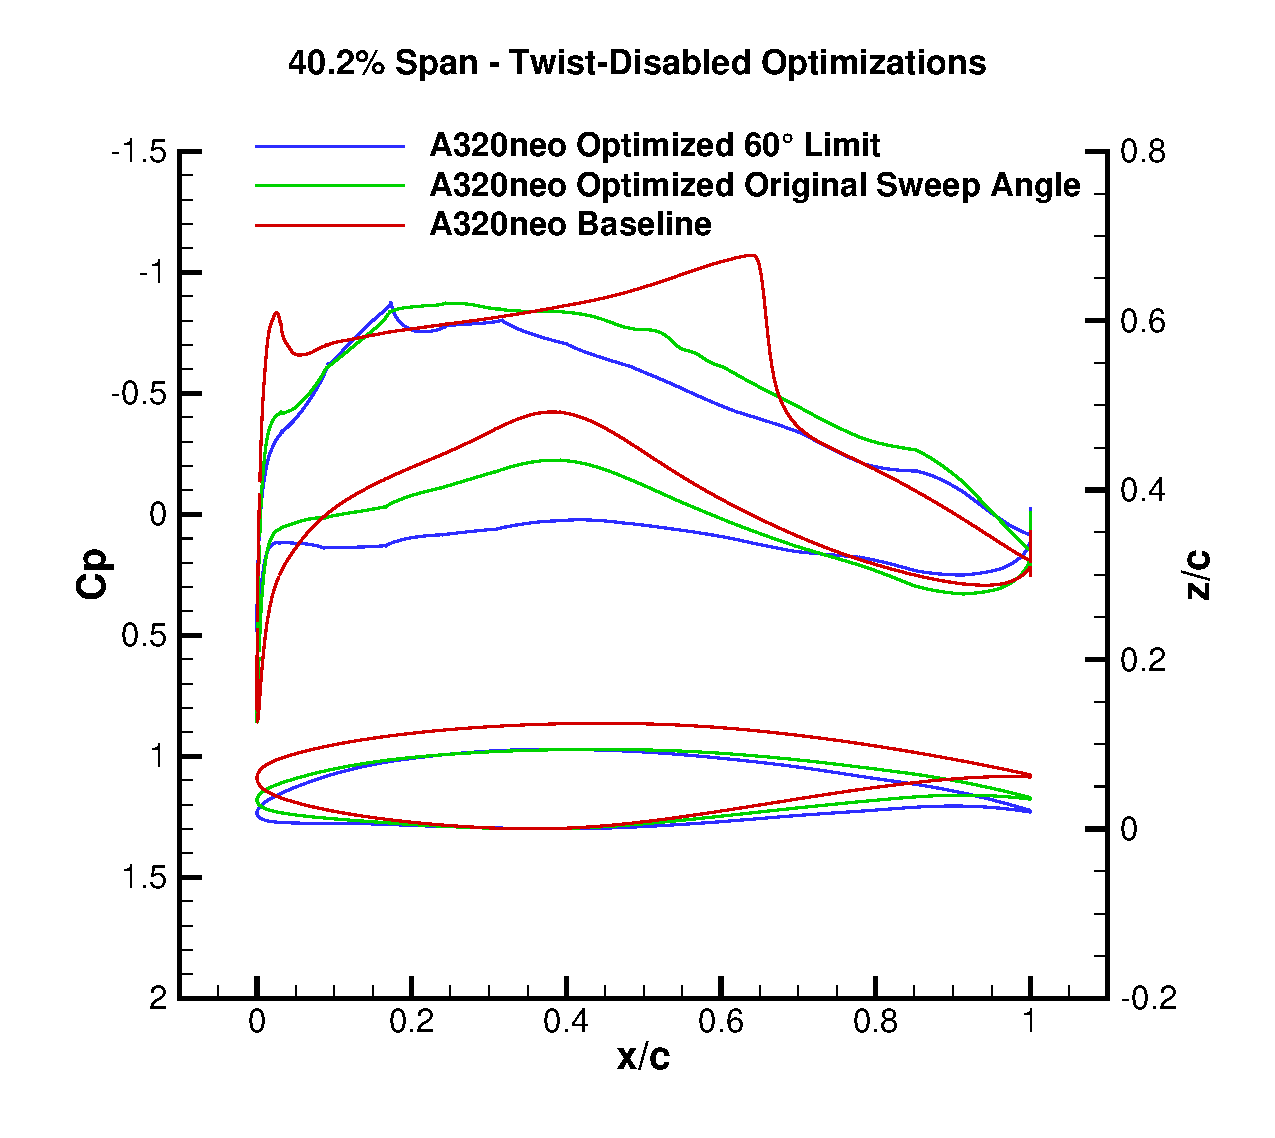
\includegraphics[trim={0.25cm 0.25cm 0.25cm 0.25cm},clip,width=3in]{Figures/No_Twist/A320neo/A320neo_Optimize_NoTwist-40.2percent_Span.eps}}
    \hspace{0.25cm}
    \subfloat[\label{fig:a320neo_notwist_section_59.8_perc}]{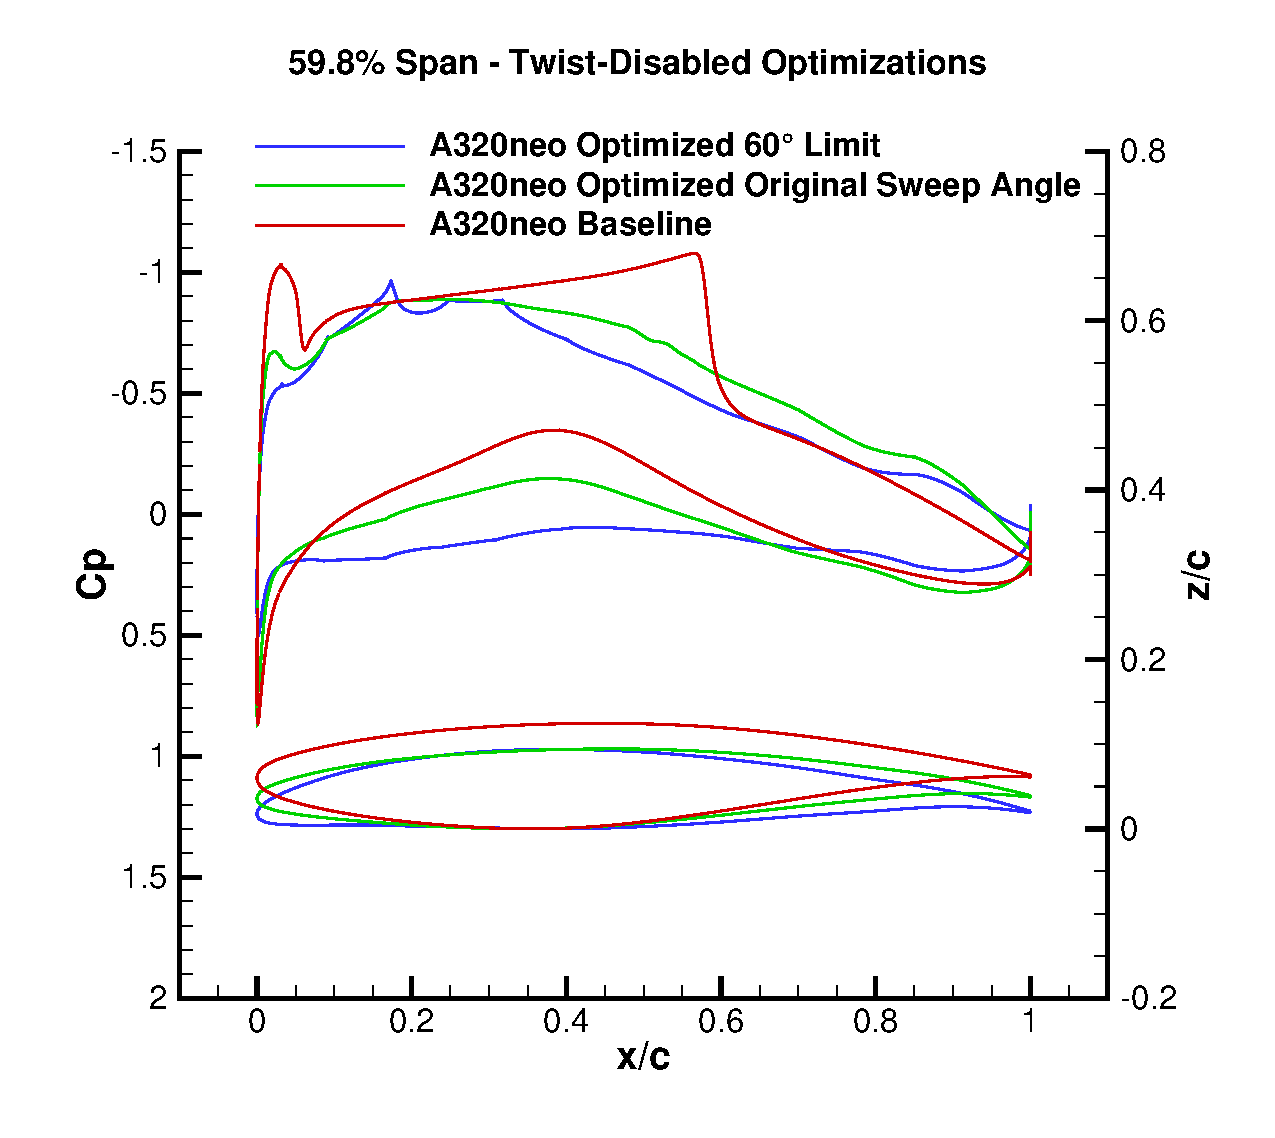
\includegraphics[trim={0.25cm 0.25cm 0.25cm 0.25cm},clip,width=3in]{Figures/No_Twist/A320neo/A320neo_Optimize_NoTwist-59.8percent_Span.eps}}\\
    \subfloat[\label{fig:a320neo_notwist_section_79.4_perc}]{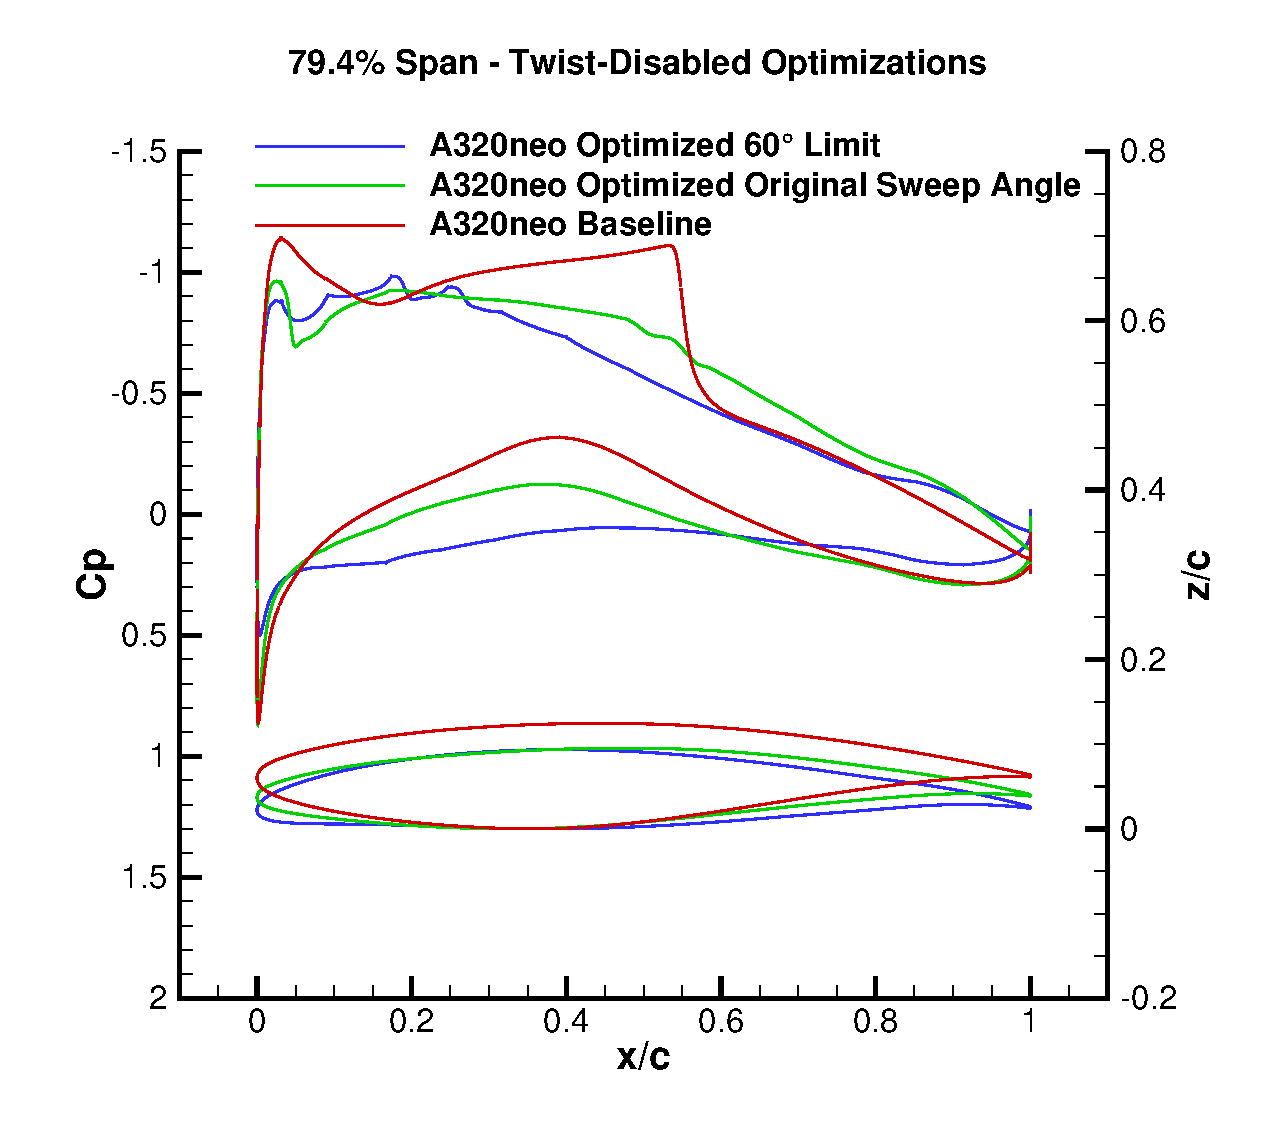
\includegraphics[trim={0.25cm 0.25cm 0.25cm 0.25cm},clip,width=3in]{Figures/No_Twist/A320neo/A320neo_Optimize_NoTwist-79.4percent_Span.eps}}
    \hspace{0.25cm}
    \subfloat[\label{fig:a320neo_notwist_section_99.0_perc}]{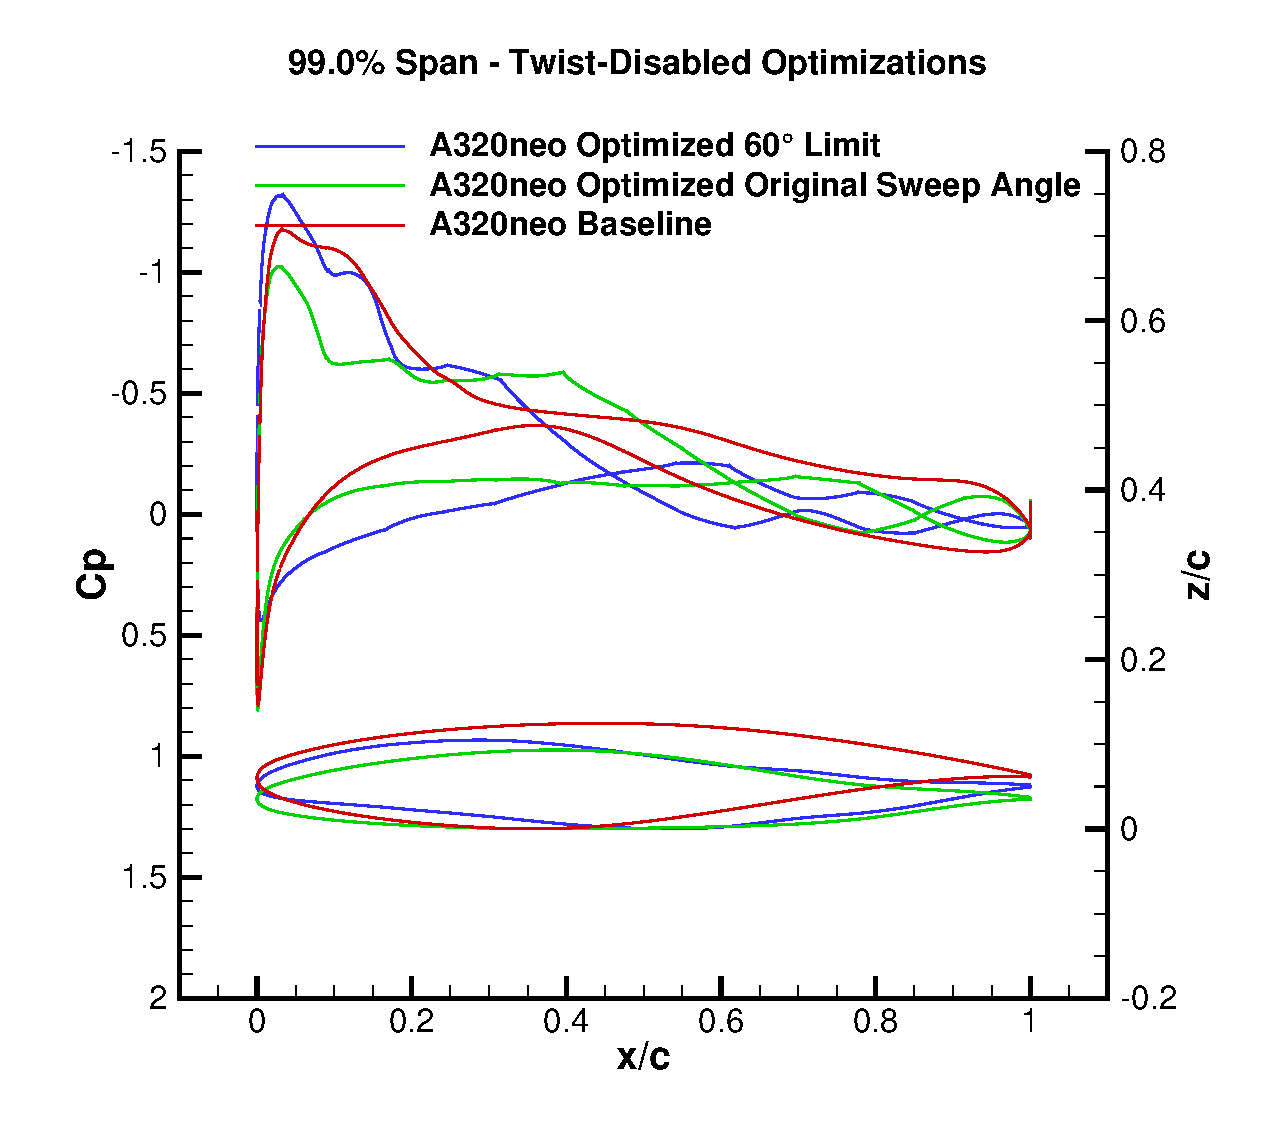
\includegraphics[trim={0.25cm 0.25cm 0.25cm 0.25cm},clip,width=3in]{Figures/No_Twist/A320neo/A320neo_Optimize_NoTwist-99.0percent_Span.eps}}
    \caption{Section geometry and pressure distribution plots of the trimmed angle of attack A320neo baseline planform and 60.0\degree\ sweep angle limit optimized planform at 1.00\% (\ref{fig:a320neo_notwist_section_1_perc}), 20.6\% (\ref{fig:a320neo_notwist_section_20.6_perc}), 40.2\% (\ref{fig:a320neo_notwist_section_40.2_perc}), 59.8\% (\ref{fig:a320neo_notwist_section_59.8_perc}), 79.4\%(\ref{fig:a320neo_notwist_section_79.4_perc}), and 99.0\% (\ref{fig:a320neo_notwist_section_99.0_perc}) span.}
\label{fig:a320neo_notwist_section_plots}
\end{figure}
\FloatBarrier

The A320neo ASO cases without wing twist are able to eliminate the sharp drop in pressure that occurs between 60-80\% of the local chord on the upper surface of the wing in Figure~\ref{fig:a320neo_section_plots}. This is especially notable in the fixed sweep angle optimization at 27.9\degree, which achieves this without any increase to the sweep angle. The absence of a shock on the optimized wings suggests that the wave drag has been eliminated.

Compared to the NASA CRM cases without wing twist, the A320neo cases do not possess as smooth of a pressure recovery. The leading edge of the wing exhibits many perturbations in the pressure coefficient as it approaches peak suction over the upper surface. The pressure recovery is also not nearly as smooth as that exhibited in the CRM twist-deactivated cases. However, both A320neo cases without twist are able to eliminate the adverse pressure gradient that is observed on the leading half of the airfoil in the trimmed baseline case, and have achieved a favourable pressure gradient past 20\% of the local chord.

Comparing between the 60.0\degree\ sweep limit case without twist and the fixed sweep angle optimization at 27.9\degree\ shows that the latter case achieves many of the performance characteristics of the former without an increase in the wing's sweep angle. Nevertheless, the pressure recovery for the optimized planform at the original sweep angle of 27.9\degree\ is not as smooth, with many small pressure perturbations over the upper surface of the wing past 40\% local chord along the entire wingspan, although it is unclear why this has occurred.

The section shapes for both the 27.9\degree\ fixed sweep angle and 60.0\degree\ sweep limit optimizations are very similar, which mirrors the behaviour observed in the the previous A320neo ASO cases, as well as the CRM ASO cases without wing sweep. The root section shape is substantially thicker for both optimized wings compared to the initial geometry, as seen in Figure~\ref{fig:a320neo_notwist_section_1_perc}. The thickness decreases along the remainder of the wingspan to become thinner than the initial geometry. This result agrees well with the results of other studies~\cite{ledoux_study_2015, kenway_multipoint_2015, telidetzki_application_2014, lyu_rans-based_2014, lyu_aerodynamic_2015, osusky_drag_2015, shi-dong_approximate_2018, yu_influence_2018, koo_investigation_2018}, as the minimum volume constraint incites this behaviour so as to create a thin outboard wing. 
% The section shape between the root and outboard section differs dramatically compared to the A320neo ASO cases with twist. When twist is disabled, the mid-wing section shape becomes substantially thinner, with both the leading and trailing edge dropping down while the upper and lower section between 20-60\% local chord flattens out.
The mid-chord sections reduces are flattened, while the leading and trailing edge have been lowered. This trailing edge does not appear to have lowered as much as the leading edge, giving the appearance that the local twist on the wing has changed. This behaviour suggests that the optimizer is attempting to modify the local twist on the wing without violating the twist equality constraint of 0\degree. Similar behaviour appeared in the CRM ASO cases without wing twist.

Yet again, the strange behaviour is exhibited at the wingtip. In both the 27.9\degree\ sweep angle and 60.0\degree\ sweep limit cases without wing twist, the optimizer has produced a section shape with a reflexed camber line, as seen in Figure~\ref{fig:a320neo_notwist_section_99.0_perc}. 
% Positive camber is exhibited before 50\% local chord, while negative camber is exhibited aft of it. This behaviour was demonstrated in all other optimization cases for both the A320neo and the NASA CRM. 
Since changes to wing twist were not permitted in these 27.9\degree\ sweep angle and 60.0\degree\ sweep limit cases, it appears that this behaviour must result from other design variables. It is unclear what the origin of this behaviour is, and a thorough search of relevant literature did not produce any studies with similar results.

The results of the ASO on the A320neo at a fixed sweep angle of 27.9\degree\ and a sweep limit of 60.0\degree\ without wing twist are not directly comparable to other studies. A search of relevant literature did not produce ASO studies on the A320neo on a similar basis to this study. Therefore, these results stand alone as novel results at the time of writing. 

\section{Drag Behavior with Varying Sweep Angles}
\label{sec:crm-drag-trends}
%%%%%%%%%%%%% TALK ABOUT DISCRETE ANGLE STUDY HERE %%%%%%%%%%%%%
The characterization of the aircraft drag as a function of the sweep angle was conducted as described in section~\ref{sssec:drag-opt-methods}. The ASO on the CRM wing was conducted at fixed sweep angles with local wing twist disabled, but with angle of attack and section shape included. The disabling of local wing twist as a design variable corresponds to a local twist equality constraint of 0\degree. This choice of design variables was made in consideration of the geometry artifacts on the CRM wing that are produced when local twist changes are permitted, as in section~\ref{ssec:crm-opt-twist}. The ASO case without wing twist at the original sweep angle of 37.5\degree\ is identical to that conducted in section~\ref{ssec:crm-opt-notwist}, such that it will be reused here. The trimmed baseline case presented in section~\ref{ssec:crm-opt-twist} and the 60.0\degree\ sweep limit case without wing twist in section~\ref{ssec:crm-opt-notwist} were also used for comparison in this study. The resultant parameters for the remaining cases to be run at fixed sweep angles of 40.0\degree\ and 42.5\degree\ are presented in Table~\ref{tab:crm_drag_trend_study}, with all other parameters remaining unchanged as presented in Table~\ref{tab:crm-opt}.

Both the 40.0\degree\ and 42.5\degree\ fixed-sweep angle CRM ASO cases converged very smoothly. Qualitative analysis of the merit function, optimality, and feasibility demonstrated that the 40.0\degree\ case converged after 330 design iterations, whereas the 42.5\degree\ case converged after 288 design iterations, as seen in Figures~\ref{fig:crm_notwist_converge_40.0_Deg} and~\ref{fig:crm_notwist_converge_42.5_Deg}, respectively. The 40.0\degree\ case exhibited a decrease in the drag coefficient $C_D S$ by 55 drag counts compared to the trimmed baseline, but only decreased by 2.5 drag counts compared to the ASO at the original (37.5\degree) sweep angle, as seen in Table~\ref{tab:crm_drag_trend_results}. The angle of attack increased by 2.4\degree\ to 39.90\degree\ compared to the trimmed baseline planform, and by approximately 2.6\degree\ relative to the 37.5\degree\ ASO case. The moment coefficient $C_M S$ decreased moderately by 0.227 to -2.931 compared to the trimmed baseline planform, and by 0.214 compared to the 37.5\degree\ ASO case. The $L/D$ increased by almost 3 counts compared to the trimmed baseline planform, but only increased by 0.15 compared to the ASO at the original sweep angle. The 40.0\degree\ case performed 9.316\% better relative to the trimmed baseline and 0.460\% better relative to the optimization at the original sweep angle, using the drag coefficient as the basis of comparison.

\begin{table}[!tp]
\centering
\caption{Modified design variable constraints for CRM 40.0\degree\ and 42.5\degree\ drag behaviour study optimization cases.}
\label{tab:crm_drag_trend_study}
\begin{tabular}{lrrrr}
\hline\hline
Constraint & \multicolumn{2}{c}{40.0\degree\ Fixed Sweep Angle} & \multicolumn{2}{c}{42.5\degree Fixed Sweep Angle}\\ \hline
 & \multicolumn{1}{c}{Lower Limit} & \multicolumn{1}{c}{Upper Limit} & \multicolumn{1}{c}{Lower Limit} & \multicolumn{1}{c}{Upper Limit}\\ \hline
Local Twist & 0\degree & 0\degree & 0\degree & 0\degree \\
Leading Edge Sweep Angle & 40.0\degree & 40.0\degree & 42.5\degree & 42.5\degree \\ \hline\hline
\end{tabular}
\end{table}


%%%%%% CRM NO TWIST DRAG TREND CONVERGENCE PLOTS %%%%%%
\begin{figure}[!tp]
\centering
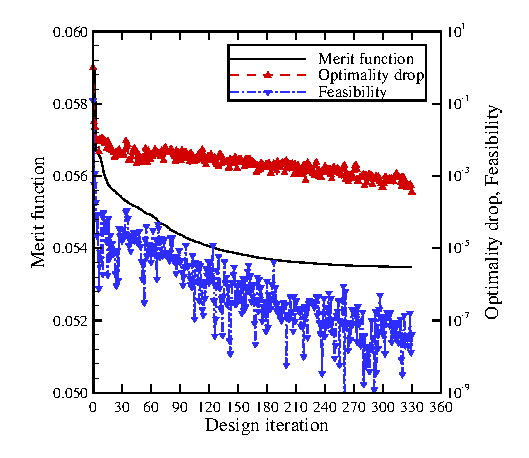
\includegraphics[width=4.5in]{Figures/No_Twist/NASA_CRM/Optimize_CRM_FIXED_No_Twist_40.0deg.eps}
\caption{Convergence history for NASA-CRM optimization without wing twist and an upper sweep angle limit of 40.0\degree.}
\label{fig:crm_notwist_converge_40.0_Deg}
\end{figure}

\begin{figure}[!tp]
\centering
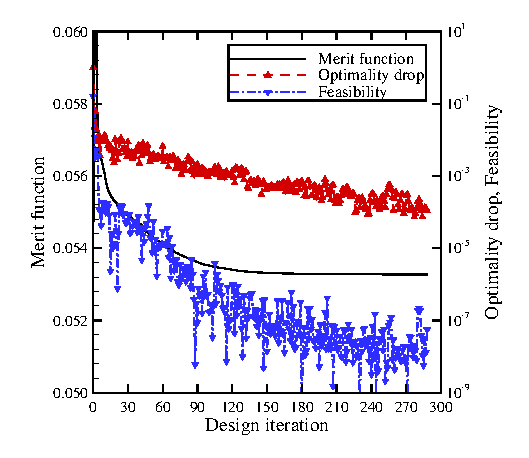
\includegraphics[width=4.5in]{Figures/No_Twist/NASA_CRM/Optimize_CRM_FIXED_No_Twist_42.5deg.eps}
\caption{Convergence history for NASA-CRM optimization without wing twist and an upper sweep angle limit of 42.5\degree.}
\label{fig:crm_notwist_converge_42.5_Deg}
\end{figure}

%%%%%%% TABLE OF RESULTS %%%%%%%
\begin{table}[!tp]
\centering
\caption{Results summary for the optimization of the NASA CRM without wing twist at varying wing sweep angles}
\label{tab:crm_drag_trend_results}
\begin{adjustbox}{center}
\begin{tabular}{lccccc}
\hline\hline
Design Variable & Trimmed Baseline & \makecell{Original (37.5\degree)\\Sweep Angle} & \makecell{40.0\degree\\Sweep Angle} & \makecell{42.5\degree\\Sweep Angle} & \makecell{60.0\degree\\Sweep Limit}\\
\hline
$S$ (ref. units\textsuperscript{2}) & 3.395 & 3.394 & 3.394 & 3.393 & 3.393\\
$C_L S$ & 1.6972 & 1.6972 & 1.6972 & 1.6972 & 1.6972\\
$C_M S$ & -2.704 & -2.717 & -2.931 & -3.148 & -3.742 \\
$C_D S$ (counts) & 589.7 & 537.2 & 534.7 & 532.7 & 531.1\\
$L/D$ & 28.78 & 31.59 & 31.74 & 31.86 & 31.96\\
Angle of Attack & 1.982\degree & 1.771\degree & 1.802\degree & 1.904\degree & 2.225\degree \\[0.25cm]
\makecell[l]{Post-Optimization\\Leading Edge Sweep Angle} & 37.50\degree & 37.31\degree & 39.90\degree & 42.40\degree & 48.50\degree \\[0.5cm]
\makecell[l]{Change in $C_D S$\\Relative to Trimmed Baseline} & 0.000\% & -8.897\% & -9.316\% & -9.663\% & -9.936\% \\[0.5cm]
\makecell[l]{Change in $C_D S$\\Relative to Optimization at\\Original (37.5\degree) Sweep Angle} & 11.03\% & 0.000\% & -0.460\% & -0.841\% & -1.141\% \\
\hline\hline
\end{tabular}
\end{adjustbox}
\end{table}

The 42.5\degree\ sweep angle ASO case displayed an almost linear improvement over the 40.0\degree\ case, relative to the optimization at the original sweep angle. The drag coefficient decreased by 57 drag counts compared to the trimmed baseline and decreased by 4.5 drag counts compared to the ASO at the original (37.5\degree) sweep angle. The angle of attack increased by 4.9\degree\ over the trimmed baseline and by 5.1\degree\ over the optimization at 37.5\degree. The moment coefficient decreased further, decreasing by 0.444 and 0.431 relative to the trimmed baseline and 37.5\degree\ case, respectively. The $L/D$ increased by just over 3 and 0.1 counts relative to the trimmed baseline and 37.5\degree\ case, respectively. The 42.5\degree\ case performed 9.663\% better relative to the trimmed baseline and 0.841\% better relative to the optimization at the original sweep angle, using the drag coefficient as the basis of comparison. The changes in almost all performance metrics represents a sub-linear increase in performance, and is very nearly linear.

Plots of the changes in the drag coefficient $C_D S$ by drag count for the trimmed baseline, optimized cases at fixed sweep angles, and the 60.0\degree\ sweep limit cases are given in Figure~\ref{fig:crm_drag_trend_abs}. The change in drag coefficient relative to the trimmed baseline CRM wing is given in Figure~\ref{fig:crm_drag_trend_perc_baseline}, which illustrates that the biggest performance improvements are obtained without having to include wing sweep as a design variable, wherein an 8.9\% reduction in drag is obtained. Using the wing optimized at the original sweep angle as the basis of comparison places the results into context, wherein one can clearly see the almost linear benefits in drag reduction for initial increases in the sweep angle in Figure~\ref{fig:crm_drag_trend_perc_opt_baseline}. Calculating the rate of change in drag between the 37.5\degree\ and 40.0\degree\ optimization results produces a 0.18\% decrease in drag per 1\degree\ increase in sweep, or a decrease in 1 drag count per degree.

This slope decreases with further increases in sweep, evidenced by the -0.15\% per degree decrease in drag obtained between the 40.0\degree\ and 42.5\degree\ optimized wings. The slope continues to decrease between the 42.5\degree\ sweep angle and 60.0\degree\ sweep limit cases, the latter of which produces 48.50\degree\ sweep angle wing. The rate of change of drag in this section is -0.120\% per degree, which is far lower than the slope at the initial sweep angle changes.


% Drag trend plot
\begin{figure}[!tp]
\centering
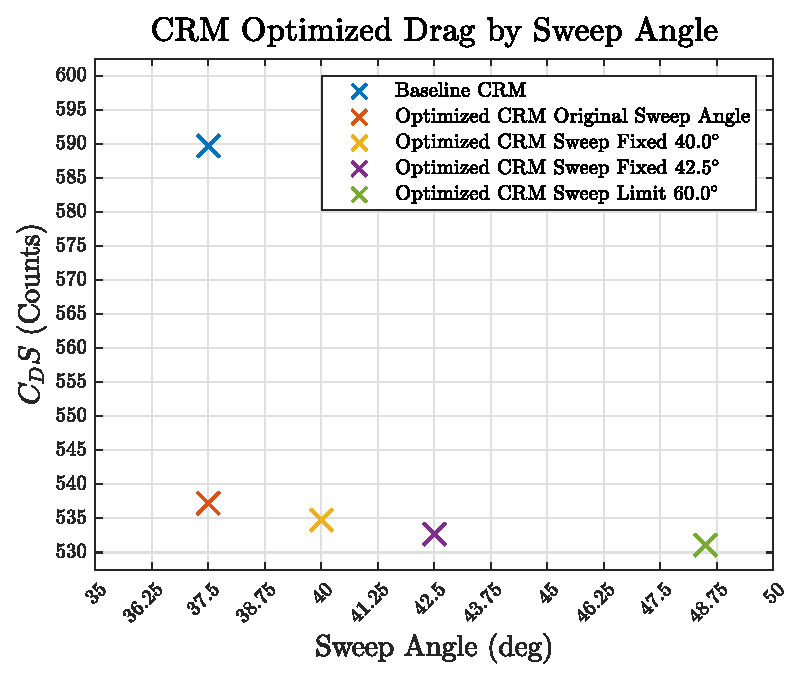
\includegraphics[width=4.5in]{Figures/Drag_Trend/crm_drag_trend.eps}
\caption{Plot of $C_{D} S$ by sweep angle for baseline, fixed sweep angle [37.5, 40.0, 42.5], and varying sweep angle (60.0\degree\ limit) optimization cases.}
\label{fig:crm_drag_trend_abs}
\end{figure}

\begin{figure}[!tp]
\centering
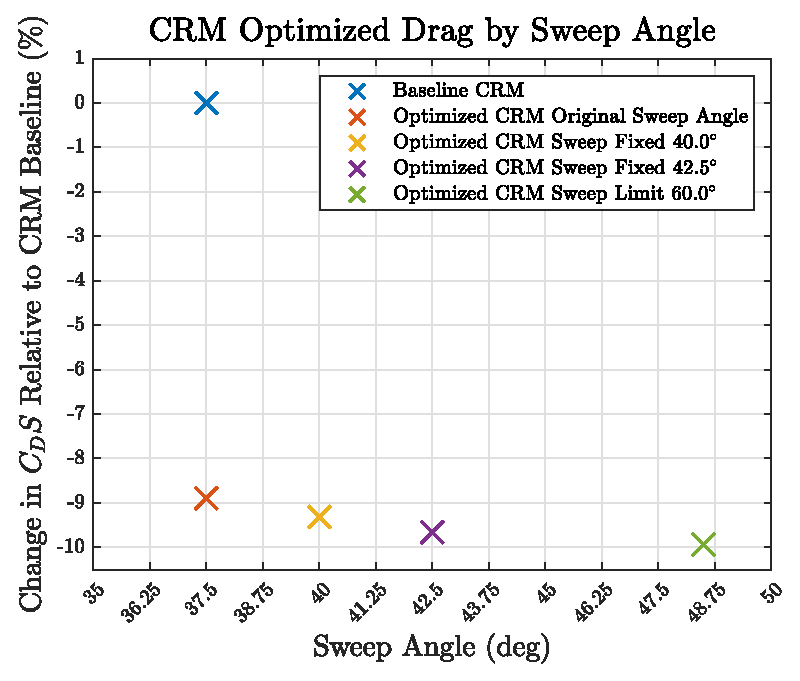
\includegraphics[width=4.5in]{Figures/Drag_Trend/crm_drag_trend_perc.eps}
\caption{Plot of percent change in $C_{D} S$ by sweep angle relative to baseline CRM configuration for trimmed baseline, fixed sweep angle [37.5, 40.0, 42.5], and varying sweep angle (60.0\degree\ limit) optimization cases.}
\label{fig:crm_drag_trend_perc_baseline}
\end{figure}

\begin{figure}[!tp]
\centering
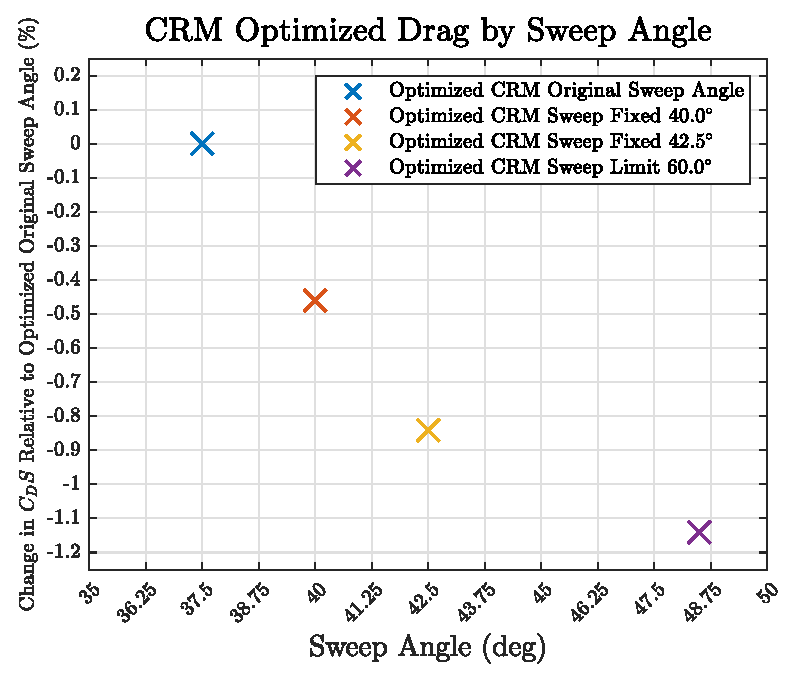
\includegraphics[width=4.5in]{Figures/Drag_Trend/crm_drag_trend_perc_2.eps}
\caption{Plot of percent change in $C_{D} S$ by sweep angle relative to CRM optimized at original sweep angle for fixed sweep angle [37.5, 40.0, 42.5] and varying sweep angle (60.0\degree\ limit) optimization cases.}
\label{fig:crm_drag_trend_perc_opt_baseline}
\end{figure}
\FloatBarrier